
%%%%%%%%%%%%%%%%%%%%%%%%%%%%%%%%%%%%%%%
% Modeling LISA tilt-to-length(TTL) coupling with HG modes.
%%%%%%%%%%%%%%%%%%%%%%%%%%%%%%%%%%%%%%%

%%%%%%%%%%%%%%%%%%%%%%%%%%%%%%%%%%%%%%%
\documentclass[aps,twoside,secnumarabic,balancelastpage,amsmath,amssymb,nofootinbib,hyperref=pdftex]{revtex4}
\usepackage{refstyle}
\usepackage[x11names]{xcolor}
\usepackage{caption}
\captionsetup{compatibility=false}
\usepackage{amsmath}
\usepackage{subcaption}
\usepackage[labelformat=parens,labelsep=quad, skip=3pt]{caption}
\usepackage{float}
\usepackage{chapterbib} 
\usepackage{graphics}     
\usepackage[pdftex]{graphicx}     
\usepackage{epsf}        
\usepackage{bm}            %bold math
\usepackage{commath}
\usepackage{verbatim}		%comments
\usepackage{fancyhdr}		%header
\usepackage{titlesec}		%section format
\usepackage[colorlinks=true]{hyperref}  %last
\usepackage{booktabs}
%title page border
\usepackage{fancybox}


%
\definecolor{gatorblue}{RGB}{0, 33, 165}
\definecolor{gatororange}{RGB}{250,70,22}

%hf page styles
\pagestyle{fancy}
\fancyhf{}


%section format
\titleformat{\section}
{\color{gatororange}\normalfont\scshape\Large}
{\color{gatororange}\thesection}{1em}{}[\vspace{-0.5ex}%
\rule{\textwidth}{0.3pt}]



%%Header
\fancyhf{}
\setlength\headheight{14pt}
\lhead{
\textcolor{gatorblue}{\rule[-2pt]{\textwidth}{16pt}}%
\hspace{-\textwidth}%
\textcolor{white}{\tab \textbf{PauLISA}}}
\rhead{\textcolor{white}{SN \thesection}}
%%

%\fancyfoot[CE,CO]{\leftmark}
\fancyfoot[RE,RO]{\thepage}
\renewcommand{\footrulewidth}{1pt}
\renewcommand{\footrule}
{\hbox to\headwidth{\color{gatorblue}\leaders\hrule height \footrulewidth\hfill}}


%%Line
\newlength{\seplinewidth}
\newlength{\seplinesep}
\setlength{\seplinewidth}{1pt}
\setlength{\seplinesep}{2mm}
\colorlet{sepline}{gatororange}
\newcommand*{\sepline}{%
  \par
  \vspace{\dimexpr\seplinesep+.5\parskip}%
  \cleaders\vbox{%
    \begingroup %  color
      \color{sepline}%
      \hrule width\linewidth height\seplinewidth
    \endgroup
  }\vskip\seplinewidth
  \vspace{\dimexpr\seplinesep-.5\parskip}%
}
%%

%figs/caps
\graphicspath{ {figures/} }
\captionsetup{justification=raggedright,singlelinecheck=false}

%tab
\renewcommand{\arraystretch}{1}
\newcommand\tab[1][3mm]{\hspace*{#1}}

%% EQ'S REUSE
\newcommand{\Hn}{H_{n}\Big(\frac{\sqrt{2}x}{w(z)}\Big)}
\newcommand{\Hm}{H_{m}\Big(\frac{\sqrt{2}y}{w(z)}\Big)}
\newcommand{\bigfrac}[2]{\Big( \frac{#1}{#2}\Big)}
\newcommand{\floor}[1]{\left\lfloor #1 \right\rfloor}
\newcommand{\ceil}[1]{\left\lceil #1 \right\rceil}

\newcommand{\sectionend}{\clearpage \newpage \vspace{.5in}\sepline}

%%%%%%%%%%%%%%%%%%%%%%%%%%%%%%%%%%%%%%%

\begin{document}




\raggedright

\vspace{200pt}
\sepline
\title{\color{gatorblue}\Large \normalfont \scshape LISA: Tilt-to-Length Noise Coupling with Hermite-Gauss Modes}
\author{Paul Edwards}

\affiliation{University of Florida}
\begin{abstract}
\sepline\vspace{20pt}
In LISA, a critical noise source is expected to arise from small misalignments between the test mass and spacecraft optical elements, which is then coupled into angular jitter of the spacecraft itself. This noise is termed tilt-to-length (TTL) coupling noise. We model TTL noise originating from these intrinsic misalignments via interference of tilted, laterally-shifted measurement beams with on-axis reference Gaussian beams using the Hermite-Gauss model for approximately paraxial beams.
\end{abstract}



\maketitle

\begin{figure}[hb]
\centering
\sepline
\begin{subfigure}{.2\textwidth}
  \centering
  \includegraphics[width=.4\linewidth]{jupyter}
\end{subfigure}%
\begin{subfigure}{.2\textwidth}
  \centering
  \includegraphics[width=.4\linewidth]{python}
\end{subfigure}
\end{figure}



\let\endtitlepage\relax




\sectionend

\tableofcontents

\sectionend

\section{LISA Overview}

Large cosmic events, such as SMBH mergers, produce measurable gravitational waves which propagate at the speed of light as strain in spacetime curvature. Gravitational waves result from a changing quadrupole moment and can be detected as a periodic distance change between two points. However, strain amplitudes at Earth approach $10^{-21}$ in gravitational waves of frequency $10^{-16}$ to $10^{4}$ Hz. Generally, gravitational wave detection entails a laser interferometry scheme to measure the path length change of light between two test masses.

\medskip

The Laser Interferometer Space Antenna (LISA) is a space-based gravitational wave detector commissioned by ESA, in collaboration with NASA and an international consortium. The project will consist of constellation of three satellites, forming an equilateral triangle, which will trail in Earth's orbit with an arm length of $\sim$2.5 million km. Each of the three satellites will house several interferometers (Spacecraft/long-arm, TM, Reference), as well as two free-falling, gold-coated test masses. Telescopes will send and receive light between the satellites. Test mass interferometers will measure path length changes between the TM and OB. The long-arm interferometer will measure path length changes between S/C. Combined, these are used to detect gravitational waves in the $10^{-4}$ to 1 Hz range (LIGO ranges 10 Hz to 10 kHz).

	\begin{figure}[hb]
	\centering
	\includegraphics[scale=.7]{fxnal}
	\caption{Functional diagram showing primary components of the OB and beam paths to local S/C backlink and transceiving far S/C. Large white blocks are TM structure, O/B, laser assembly, and TS.}
	\label{fig:fxnal}
	\end{figure}

\sectionend

\section{Tilt-to-Length Coupling Noise and Signals}

\subsection{Tilt-to-length}
In LISA, it is expected that intrinsic misalignments between the optical bench (OB) and
the attached bi-directional telescope are the main avenues for laser beam pointing noise, also known as tilt-to-length
(TTL) coupling, into the gravitational wave signal.

\medskip

Section C of the LISA Payload Description Document (PDD) outlines expected TTL couplings and tolerances: 

\begin{description}
  \item[$\bullet$ S/C jitter] $ \sim  10\; \text{nrad}/\sqrt{\text{Hz}}$
  \item[$\bullet$ OB Lateral alignment offset] $\sim 20\; \mu m$
  \item[$\bullet$ Combined] $\sim 20\; \text{pm}/\sqrt{\text{Hz}}$
\end{description}

Selection of reference beam shape and photoreceiver dimensions
can play a critical role in TTL subtraction. We model TTL coupling via interference of a tilted, misaligned beam
with a local reference beam and present differential wavefront sensing (DWS) calculations for local and received beam
shape combinations of tophat-Gaussian interference.

\medskip

\subsection{Signals Demodulation Formalism}

Using full information of the electric fields, one can determine signals produced at LISA's interferometers. Consider the sum of the receieved and reference fields 

\begin{equation}
E = E_{RX}+E_{LO}.
\end{equation}

More explicitly: 

\begin{equation}
	E = 
			E_{0(ref)} 
			e^{i(( \omega_{ref} t)+\phi_{1})} 
			u_{00}
			+
			E_{0(rec)}			
			e^{i (( \omega_{rec}t)+\phi_{2})} \; ,
\end{equation}


Demodulating and neglecting $\Delta \phi$ at the phasemeter yields an in-phase signal $I$ is

\begin{equation}
	I
	=
	E^{*}E \times \cos (\Delta \omega t) \; ,	
\end{equation}

and the quadrature phase signal $Q$ is

\begin{equation}
	Q
	=
	E^{*}E \times \sin (\Delta \omega t) \; .
\end{equation}


Therefore, after a low pass filter (as the heterodyne frequency is on the order of MHz), the phase is 

\begin{equation}
 		\phi_{beat}
 		=
 		 	\arctan	(\frac{Q}{I})	
\end{equation}


\subsection{Signals}

LISA uses PD's to measure interference of a received beam with a reference beam, resulting in heterodyne beat notes which are used to determine phase difference ($\phi_{beat} = \phi_{1}-\phi_{2}$) of the two beams. Fields of the reference Gaussian beam (LO) and received tophat beam (RX) defined with a basis $(w_{0},z_{0})$ are, respectively:

\begin{equation} \label{eq:19}
	E_{LO} = 
		E_{0\; (LO)} e^{i(( \omega_{LO} t)+\phi_{1})}
		u_{00}(w_{0\; LO},z_{0\; LO})	
	\;,
\end{equation}

and

\begin{equation} \label{eq:18}
	E_{RX} = 
		E_{0\; (RX)} e^{i (( \omega_{RX}t)+\phi_{2})} 			
		\sum_{n,m=0}
		c_{nm}u_{nm}(w_{0\; RX},z_{0\; RX}) 		
	\;,
\end{equation}
	
where $c_{nm}$ represent coeffients relative to modes $n$ and $m$ of an electric field spatial component $u_{nm}$, and $w_0$ and $z_0$ represent beam waist and waist location.\\

Power at the PD, given an electric field $E$, is

\begin{align*}
P_{pd} =& \int_{-\infty}^{\infty}\int_{\infty}^{\infty} E^* E dx dy
\\=&	 \int_{- \infty}^{\infty}\int_{- \infty}^{\infty}[
E_{LO}^*E_{LO}+E_{RX}^*E_{RX}+E_{RX}^*E_{LO}+E_{RX}E_{LO}^*]
\\=&	 \int_{- \infty}^{\infty}\int_{- \infty}^{\infty}[
P_{LO} + P_{RX} + E_{RX}^*E_{LO}+E_{RX}E_{LO}^*]
\end{align*}

The only A/C component comes from the second two terms, so the beat note signal is obtained from the argument of its power (with bounds assuming the PD area is large relative to the beam)

\begin{equation}\label{eq:20}
	\phi_{beat}= \arg \Big[
	 \int_{- \infty}^{\infty}\int_{- \infty}^{\infty} E_{LO}^*E_{RX} \; dxdy
	 \Big ]
	 \; ,
\end{equation}

For a half-plane PD, only the bounds of integration need be adjusted. For the left side of the HPPD

\begin{equation}
	\phi_{L}= \arg \Big[
	 \int_{- \infty}^{\infty}\int_{- \infty}^{0} E_{LO}^*E_{RX} \; dxdy
	 \Big ]
	 \; ,
\end{equation}

and for the right side

\begin{equation}
	\phi_{R}= \arg \Big[
	 \int_{- \infty}^{\infty}\int_{0}^{\infty} E_{LO}^*E_{RX} \; dxdy
	 \Big ]
	 \; .
\end{equation}

The DWS (Differential Wavefront Sensing) signal for a half-plane PD is calculated as a difference of right and left beat note signals:

\begin{equation}
 		\Phi_{DWS} 
 		=
 		 	[\phi_R - \phi_L]
\end{equation}


The LPS (Longitudinal Pathlength Signal) For HPPD is calculated as:

\begin{equation}
 		\Phi_{LPS} 
 		=
 		 	\frac{1}{2}[\phi_R + \phi_L]
\end{equation}

The spatial component of the electric fields can be formulated using Hermite-Gauss modes.

\sectionend

\section{Hermite-Gauss Modes}

\subsection{HG Modes Overview}
Hermite-Gauss (HG) modes represent a set of exact solutions of the paraxial wave equation 

\begin{equation}
	\nabla_{t}^2u(x,y,z)-2ik\partial{z}u(x,y,z)=0 \; .
\end{equation}

The Living Reviews article \citep{Bond} gives the general expression for HG modes as
	
	\begin{equation} \label{eq:1}
		u_{nm}(x,y,z)=(2^{n+m-1}n!m!\pi)^{-1/2}
		\frac{1}{w(z)}H_{n} \Big( \frac{\sqrt{2}x}{w(z)} \Big)
		H_{m} \Big(\frac{\sqrt{2}y}{w(z)} \Big)
		\exp 
		\Big(
		\frac{-ik(x^{2}+y^{2})}{2R_{c}(z)}
		-\frac{x^{2}+y^{2}}{w(z)^{2}} 
		+i(n+m+1)\arctan(\Psi(z))	
		\Big)\;,
	\end{equation}
	
where $\Psi(z) = \arctan(\frac{z-z_0}{z_R})$ is the Gouy phase. In terms of the Gaussian beam parameter,
	
	\begin{equation} \label{eq:2}
		q(z)=iz_{R}+z-z_{0}=q_{0}+z-z_{0}\;,
	\end{equation}
	
	HG modes may be expressed as (where $w(z)=w_0 \sqrt{1+\bigfrac{z-z_0}{z_R}^2}$):
	
	\begin{align} \label{eq:3}
		u_{nm}(x,y,z)=& u_{n}(x,z)u_{m}(y,z)
		\nonumber\\=& 
		\Big(\frac{2}{\pi}\Big)^{1/4}
		\Big(\frac{1}{2^{n}n!w_{0}}\Big)^{1/2}
		\Big(\frac{q_{0}}{q(z)}\Big)^{1/2}
		\Big(\frac{q_{0}q*(z)}{q_{0}*q(z)}\Big)^{n/2}
		\Hn
		\exp\Big(\frac{-ik(x^{2})}{2q_{z}}\Big)
		\times u_{m}(y,z)
		\;,
	\end{align}
where the first four Hermite polynomials  are given by	

\[
  H_{n}(x)=\begin{cases}
               1 \tab\tab\tab\tab\tab\;\;(n=0)\\
               2x \tab\tab\tab\tab\;\;\;(n=1)\\
               4x^{2}-2 \tab\tab\;\;(n=2)\\
               8x^{3}-12x \tab\;\;(n=3)
            \end{cases}
\]

The HG modes are orthonormal, such that

\begin{equation}
	\int \int dx dy \; u_{nm} u_{n'm'}^* = \delta_{nn'} \delta_{mm'}.
\end{equation}

The Hermite polynomials can be derived from recurrence relations:
\begin{equation*}
	H_n(x) =
		n! \sum_{\nu=0}^{\lfloor{\frac{n}{2}}\rfloor}
		\frac{(-1)^\nu}{\nu!(n-2\nu)!} 
		\frac{x^{n-2\nu}}{2^\nu}
\end{equation*}

\sectionend

\subsection{General Coupling into Higher Order HG Modes via Transverse Coordinate Dependence}








In general, modes with a spatial component prefactor (e.g., $x$ and $x^2$) can be written as higher order modes. 

For $x$:

\begin{equation}\label{scatter_x}
x u_{n,m} = \frac{w_0}{2}
\Big[
	(1 - i \frac{z}{z_R})
	\sqrt{n+1} u_{n+1,m}
	+
	\sqrt{n}
	(1+i \frac{z}{z_R})
	u_{n-1,m}
\Big]
\end{equation}

Splitting these factors (ignoring $u_{n,m}$ into two terms:

\begin{equation}
X_+^1 = \frac{w_0}{2}
\Big[
	(1 - i \frac{z}{z_R})
	\sqrt{n+1} 
\Big]
\end{equation}

\begin{equation}
X_-^1 = \frac{w_0}{2}
\Big[
	\sqrt{n}
	(1+i \frac{z}{z_R})
\Big]
\end{equation}

For $x^2$:

\begin{equation}\label{scatter_x2}
x^2 u_{n,m} = \frac{w_0^2}{4}
\Big[
	(1 - i \frac{z}{z_R})^2
	\sqrt{(n+1)(n+2)} u_{n+2,m}
	+
	(2n+1)
	(1+ (\frac{z}{z_R})^2)
	u_{n,m}
	+
	\sqrt{n(n-1)}
	(1+i \frac{z}{z_R} )^2
	u_{n-2,m}
\Big]
\end{equation}

Splitting these factor into three terms:

\begin{equation}
X_-^2 = \frac{w_0^2}{4}
\Big[
	\sqrt{n(n-1)}
	(1+i \frac{z}{z_R} )^2
\Big]
\end{equation}

\begin{equation}
X_0^2 = \frac{w_0^2}{4}
\Big[
	(2n+1)
	(1+ (\frac{z}{z_R})^2)
\Big]
\end{equation}

\begin{equation}
X_+^2 = \frac{w_0^2}{4}
\Big[
	(1 - i \frac{z}{z_R})^2
	\sqrt{(n+1)(n+2)}
\Big]
\end{equation}

For approximations used in later sections, it is useful to express higher-order modes in terms of the fundamental mode. 

At the waist(if $z=z_0=0$) with an $x$ factor, this is

\begin{equation}
x u_{n,m} = \frac{w_0}{2}
\Big[
	\sqrt{n+1} u_{n+1,m}
	+
	\sqrt{n}
	u_{n-1,m}
\Big]
\end{equation}

For $n=0,1,2$ and $m=0$ at the beam waist(letting $z_{0}=0$):

\begin{equation}\label{eq:4}
u_{00}(x,y,0)= \sqrt{\frac{2}{\pi}}
\bigfrac{1}{w_{0}}
\exp \left[ - \bigfrac{x^{2}+y^{2}}{w_{0}^{2}} \right] \; ,
\end{equation}

\begin{equation}\label{eq:5}
u_{10}(x,y,0)= \sqrt{\frac{2}{\pi}}
\bigfrac{2x}{w_{0}^{2}}
\exp \left[ - \bigfrac{x^{2}+y^{2}}{w_{0}^{2}} \right] \; ,
\end{equation}

\begin{equation}\label{eq:6}
u_{20}(x,y,0)= \sqrt{\frac{2}{\pi}}
\left[ \bigfrac{2 \sqrt{2}x^{2}}{w_{0}^{3}}- \frac{\sqrt{2}}{2 w_0} \right]
\exp \left[ - \bigfrac{x^{2}+y^{2}}{w_{0}^{2}} \right] \; ,
\end{equation}

Expressing $u_{10}$ and $u_{20}$ in terms of $u_{00}$ at the beam waist (neglect $u_{n-1,m} or u_{n-2,m}$ terms in the general equations above),

	\begin{equation}\label{eq:7}
		u_{10}(x,y,0)= \frac{2x}{w_{0}} u_{00}(x,y,0)
	\end{equation}	
	
	\begin{equation}\label{eq:8}
		u_{20}(x,y,0)= \left[2 \sqrt{2} \bigfrac{x^{2}}{w_{0}^{2}}- \frac{\sqrt{2}}{2} \right] u_{00}(x,y,0)
	\end{equation}	
	
	In PauLisa.py, Eq. \ref{eq:1} is represented by the \textit{calculate} function and Eq. \ref{eq:3} as \textit{calculate\_q}. The outputs of both functions agree exactly. In the appendix, intensity profiles produced by PauLisa.py for $u_{00}$ to $u_{33}$ are shown in Fig. \ref{fig:A1}.	

\rule{\textwidth}{0.4pt}

The spatial component of the field in the Hermite-Gaussian representation is

\begin{equation}
	E(x,y,z) = 
	e^{-ikz} \sum_{n,m} C_{n,m} u_{n,m}(x,y,z)
\end{equation}

where $C_{n,m}$ are mode coefficients, and $u_{n,m}$ are the Hermite-Gaussian modes,

	\begin{equation} \label{eq:hg}
		u_{n,m}(x,y,z)=(2^{n+m-1}n!m!\pi)^{-1/2}
		\frac{1}{w(z)}H_{n} \Big( \frac{\sqrt{2}x}{w(z)} \Big)
		H_{m} \Big(\frac{\sqrt{2}y}{w(z)} \Big)
		\exp 
		\Big(
		\frac{-ik(x^{2}+y^{2})}{2R_{c}(z)}
		-\frac{x^{2}+y^{2}}{w^{2}(z)} 
		+i(n+m+1)\psi(z))	
		\Big)\;.
	\end{equation}

The goal is to simplify Taylor expansions of off-axis HG modes following coordinate transformations, such as the $z$-coordinate transformation from a beam rotation to first order in the rotational angle $\alpha$,

\begin{align*}
z \rightarrow z-x\alpha, \mathrm{(first-order\;rotation)}
\end{align*}

which results in transverse coordinate (i.e., $x$) dependence in the coupling coefficient,

\begin{align*}
	u_{nm}(x,y,z) e^{ikx\alpha}
	\rightarrow &
	u_{nm}(x,y,z)+(ik \alpha x)u_{nm}(x,y,z).
\end{align*}

The overall coupling coefficient is $ik\alpha x$. For purposes of signal calculation, the $ik\alpha$ factor can be viewed a constant prefactor to an otherwise pure HG mode. However, transverse coordinate factors $x$ can be viewed to couple directly into the hermite polynomial , $H_n (\frac{\sqrt{2} x}{w(z)})$ (they're the only $x$-dependence outside of the exponential functions).
This results in a splitting of the hermite polynomial into a sum of higher and lower order polynomials. The following equivalence, for example, substitutes a polynomial with a factor of linear $x$-dependence for higher and lower order polynomials (proven Section 2):

\begin{equation}\label{eq:3}
x H_n(\frac{\sqrt{2}x}{w(z)}) =
	\frac{\sqrt{2} w(z)}{4}
	H_{n+1}(\frac{\sqrt{2}x}{w(z)})
	+
	\frac{\sqrt{2} w(z) n}{2} H_{n-1} (\frac{\sqrt{2}x}{w(z)})
\end{equation}


This isn't enough to transform $x u_{n,m} \rightarrow u_{n-1,m}$, for example, because other factors in the HG modes have dependence on index $n$. However, any $u_{n,m}$ with a factor of $x$ to any order can be rewritten purely as higher and lower order modes to some "constant" prefactor. Do this by defining a set of pseudo-operators $X_\pm^K$ for $x$, our coordinate of unidirectional offset. For example, a linear factor would follow

\begin{equation}
x u_{nm} (x,y,z) = 
	X_+^1 u_{n+1,m}(x,y,z)
	+
	X_-^1 u_{n-1,m}(x,y,z) 
\end{equation}

where $X_+^1$ represents a coupling from $u_{nm}$ up to $u_{n+1,m}$ and $X_-^1$ represents a coupling from $u_{nm}$ down to $u_{n-1,m}$. This notation makes it simpler to trace back to the original mode. \\

A quadratic factor in $x$ would follow (proven later),

\begin{equation}
x^2 u_{n, m} =
	X_-^2 u_{n+2,m}
	+
	X_0^2 u_{n,m}
	+
	X_-^2 u_{n-2,m}	.
\end{equation}

Note the "self-contribution" term $X_0^2 u_{n,m}$.\\

The benefit of making these transformations is the ability to rewrite the transverse coordinate dependence as a new set of mode coefficients for pure, on-axis modes. In other words, the quadratic dependence in $x$, for example, transforms the modes relative to this new coupling and relative to an original mode coefficient $C_{n,m}$, s.t. 

\begin{align*}
C_{n+2,m} \rightarrow &C_{n+2,m} + C_{nm}X_+^2
\\
C_{nm} \rightarrow & C_{nm}X_0^2
\\
C_{n-2,m} \rightarrow & C_{n-2,m} + C_{nm}X_-^2
\end{align*}

where the transformation must be applied to all modes $u_{n,m}$ in the set of non-zero mode coefficients $C_{n,m}$.\\

As another example, suppose $C_{0,0}=C_{1,0} \neq 0$, then $\sum_{n,m} C_{n,m} x u_{n,m}$ leads to $C_{1,0} x u_{1,0}$ and $C_{0,0} x  u_{0,0}$, so that

\begin{align*}
C_{2,0} \rightarrow & C_{1,0}X_+^1
\\
C_{1,0} \rightarrow & C_{0,0}X_+^1
\\
C_{0,0} \rightarrow & C_{1,0} X_-^1
\end{align*}

To determine the additional coupling that results from incrementing or decrementing $n$ in the HG modes to match the hermite polynomial and reproduce a "pure" mode, consider an arbitrary shift in index $n$ by integer $K$: 

	\begin{align*} 
		u_{n \pm K,m}(x,y,z) \rightarrow &
		(2^{n \pm K} (n \pm K)!)^{-1/2}
		\exp(i(n\pm K)\psi(z))
				H_{n \pm K} \Big( \frac{\sqrt{2}x}{w(z)} \Big)
		\\&
		(2^{m-1}m!\pi)^{-1/2}
		\frac{1}{w(z)}
		H_{m} \Big(\frac{\sqrt{2}y}{w(z)} \Big)
		\exp 
		\Big(
		\frac{-ik(x^{2}+y^{2})}{2R_{c}(z)}
		-\frac{x^{2}+y^{2}}{w(z)^{2}} 
		+i(m+1)\psi(z))	
		\Big)\;.
	\end{align*}


The top line exhibits all $n$-dependence in the equation. Recall that the polynomial $H_{n\pm K}$ term came from $x$ coupling.
So the generalized pseudo-operator ,which itself represents the entire coupling coefficient from the $x$ factor, is

\begin{equation}
	X_{\pm }^K u_{n \pm k, m} = 
		\eta_{\pm}^K
		(2^{\mp K} )^{-1/2}
		\sqrt{\frac{(n \pm k)!}{n!} }
		\exp(\mp iK  \psi(z))
		u_{n \pm k, m}		
		\;,
\end{equation}

where $\eta_{\pm}^K$ represents the factor that comes directly from the transformation $x^{\pm K} H_n \rightarrow \eta H_{n\pm K}$ (with additional terms, and, $\eta_{\pm}^K$ is used arbitrarily to represent any of the prefactors in the right side of Eq. \ref{eq:3}, for example).\\

To summarize, a transverse coordinate dependence results in higher and lower order mode hermite polynomials to some factor $\eta_{\pm}^K$. Rewriting the rest of $u_{n,m}$ to account for the index-shifted polynomial in $n$ means also having to account for $n$-dependence in the normalization factor $(2^{n+m-1}n!m!\pi)^{-1/2}$ and the Gouy phase term, $\exp(i(n+m+1)\psi(z))$.\\





\clearpage

\subsection{Linear Transverse Coordinate Coupling}

Calculating the $\eta$ factor follows from identities on the Hermite polynomials. Hermite polynomials using Rodrigues formula, where $y^2 \equiv (ax)^2 = \frac{2 x^2}{w^2(z)}$ for the case of HG modes, are \textbf{(note y is not the y-coordinate, a is not shift as in usual notation)}:

\begin{equation}\label{eq:1}
	H_n(x) = 
		(-1)^n e^{y^2} \frac{d^n}{dy^n}e^{-y^2}
\end{equation}

so,

\begin{align*}
	H_n(\frac{\sqrt{2}x}{w(z)} )
	= 
		(-1)^n e^{({\frac{ \sqrt{2} x}{w(z)}})^2} \frac{d^n}{dy^n}e^{({\frac{ \sqrt{2} x}{w(z)}})^2},
\end{align*}

The coupling $\eta$ can be determined through deriving the HG counterpart to the identity

\begin{equation}\label{id}
	H_{n+1}(y) = 2y H_n(y) - nH_{n-1}(y)
\end{equation}

\rule{\textwidth}{0.4pt}

Start with the first derivative of Eq. \ref{eq:1}, where $D \equiv \frac{d}{dy}$:

\begin{align*}
	D H_n(y) =&
	D [ (-1)^n e^{-y^2} D^n e^{-y^2} ]
	\\=&
		(-1)^n (2y) e^{y^2} D^n e^{-y^2}
		+
		(-1)^n e^{y^2} D^{n+1} e^{-y^2}
		\\=&
		2y H_n(y)
		-
		(-1)^{n+1} e^{y^2} D^{n+1}e^{-y^2}
		\\=&
		2y H_n(y)	
		-
		H_{n+1}(y)	
\end{align*}

or

\begin{equation}\label{res1}
D H_n(\frac{\sqrt{2}x}{w(z)})
=
		2\frac{\sqrt{2}x}{w(z)} H_n(\frac{\sqrt{2}x}{w(z)})	
		-
		H_{n+1}(\frac{\sqrt{2}x}{w(z)})	
\end{equation}

\rule{\textwidth}{0.4pt}

However, an equivalent solution exists for $D H_n$ without immediately applying the $(-1)$ factor,


\begin{align*}
D H_n(y) =&
	D [ (-1)^n e^{-y^2} D^n e^{-y^2} ]
\\=&
(-1)^n
	2ye^{y^2}
	D^n e^{-y^2}
	+
	(-1)^n
	e^{y^2}
	D^{n+1}
	(e^{-y^2})
	\\=&
	2y H_n(y)
	+
	(-1)^n
	e^{y^2}
	D^{n+1}
	(e^{-y^2})
	\\=&
		2y  H_n(y)
	+
	(-1)^n
	e^{y^2}
	D^{n}
	(-2y)
	(e^{-y^2})
\end{align*}

using the general Leibniz rule, where $f = -2y$ and $g = e^{-y^2}$,

\begin{align*}
	D^n(fg)=&
	\sum_{k=0}^n {n \choose k} 
	D^k f
	D^{n-k} g	
\end{align*}

but the result after substituting $f$ and $g$ is $0$  $\forall$ $k>1$.\\

Using the Leibniz rule for the derivative in the last term then,


\begin{align*}
	D^n(fg)=&
	\sum_{k=0}^1 {n \choose k} 
	D^k f
	D^{n-k} g	
	\\=&
	{n \choose 0} 
	f D^{n} (g)
	+
	{n \choose 1}
	D(f) D^{n-1} (g)
		\\=&
	-2 y D^{n} (e^{-y^2})
	+
	n
	(-2) D^{n-1} (e^{-y^2})
\end{align*}

This means $D H_n(y)$ is

\begin{align*}
D H_n(y) 
	=&
	2 y H_n(y)
	+
	(-1)^n e^{y^2}
	[
		-2y  D^{n} (e^{-y^2})
	+
	n
	(-2) D^{n-1} (e^{-y^2})
	]
	\\=&
	2y H_n(y)
	-
	2y H_n(y)
	+
	2n H_{n-1}(y)
	\\=&
	2n H_{n-1} (y)
\end{align*}

or

\begin{equation}\label{res2}
D H_n(\frac{\sqrt{2}x}{w(z)}) 
	=
	2n H_{n-1} (\frac{\sqrt{2}x}{w(z)})
\end{equation}

\rule{\textwidth}{0.4pt}

Setting the two solutions, Eq. \ref{res1}, and Eq. \ref{res2}, equal and rewriting (again $a= \frac{\sqrt{2}}{w(z)}$),

\begin{align*}
x H_n(ax) =&
	\frac{1}{2a}
	[
	H_{n+1}(ax)
	+
	2n H_{n-1} (ax)
	]
	\\=&
		\frac{1}{2a}
	H_{n+1}(ax)
	+
	\frac{n}{a} H_{n-1} (ax)
\end{align*}

or

\begin{equation}
x H_n(\frac{\sqrt{2}x}{w(z)}) =
	\frac{\sqrt{2} w(z)}{4}
	H_{n+1}(\frac{\sqrt{2}x}{w(z)})
	+
	\frac{\sqrt{2} w(z) n}{2} H_{n-1} (\frac{\sqrt{2}x}{w(z)})
\end{equation}


Check this for $n=1$, using that $H_1(\zeta) = 2 \zeta$ for any argument $\zeta$,

\begin{align*}
xH_1(y) =&
2xy \\=& 2\frac{\sqrt{2 } x^2}{w(z)}
\end{align*}

the new solution matches,

\begin{align*}
x H_1(y) =&
	 \frac{1}{2a}H_{2}(y) +  \frac{1}{a} H_{0}(y)
	 \\=&
	 \frac{1}{2a}
	 [
	 4y^2 - 2
	 ]
	 +
	\frac{1}{a}
	 \\=&
	 \frac{w(z)}{2 \sqrt{2} }
	 [
	 4(\frac{2x^2}{w^2(z)}) - 2
	 ]
	 +
	 \frac{w(z)}{\sqrt{2} }	 
	 \\=&
	 2\frac{\sqrt{2 } x^2}{w(z)}
\end{align*}

\rule{\textwidth}{0.4pt}

With the linear result, 

\begin{equation*}
x H_n(\frac{\sqrt{2}x}{w(z)}) =
	\frac{\sqrt{2} w(z)}{4}
	H_{n+1}(\frac{\sqrt{2}x}{w(z)})
	+
	\frac{\sqrt{2} w(z) n}{2} H_{n-1} (\frac{\sqrt{2}x}{w(z)})
\end{equation*}

the prefactors $\eta$ discussed previously, which might also be written as pseudo-operators for linear $x$, are clearly

\begin{align*}
\eta_+^1 = \frac{\sqrt{2}w(z)}{4}
\end{align*}

\begin{align*}
\eta_-^1 = \frac{\sqrt{2} w(z) n}{2}
\end{align*}

Note

\begin{align*}
	\eta_- \neq \eta_+
\end{align*}

because of complicated dependence on the hermite polynomial. The factors will also be different for each higher-order $x$. However, these factors at higher orders can all be calculated following a similar procedure (shown later for quadratic $x$). \\

The coupling pseudo-operator for linear $x$ dependence is now known:


\begin{equation*}
x u_{n,m} \rightarrow
	X_+^1
	u_{n+1,m}
	+
	X_-^1
	u_{n-1,m}
\end{equation*}

where

\begin{align*}
	X_{\pm }^1 u_{n \pm 1, m} = &
		\eta_{\pm}^1	
		(2^{\mp 1} )^{-1/2}
		\sqrt{\frac{(n \pm 1)!}{n!} }
		\exp(\mp i  \psi(z)).
\end{align*}




Therefore, the overall result from $x u_{n,m}$ is

\begin{align*}
	x u_{n, m} \rightarrow &
		X_+^1 u_{n+1,m} + X_-^1 u_{n-1,m}
		\\=&
	\left[
		\frac{1}{2a}
				(2 )^{1/2}
		\sqrt{\frac{ (n+1)!}{ n!} }
		\exp(-i  \psi(z))
		\right]
		u_{n+1,m}		
		\\ & + 
		\left[
		\frac{n}{a}
				(2 )^{-1/2}
		\sqrt{\frac{ (n-1) !}{n!} }
		\exp( i \psi(z))
		\right]
		u_{n-1,m}
		\\ = &
	\left[
		\frac{w(z)}{2}
		\sqrt{n+1 }
		\exp(-i  \psi(z))
	\right]
		u_{n+1,m}		
		\\  & +
		\left[
		\frac{w(z)}{ 2}
		 \sqrt{n} 
		\exp( i \psi(z))
		\right]
		u_{n-1,m} 
		\\= & 
			\left[
		\frac{w_0}{2}
		\sqrt{n+1 }
		(1-i\frac{z}{z_R} )
	\right]
		u_{n+1,m}		
		\\& + 
		\left[
		\frac{w_0}{ 2}
		 \sqrt{n} 
		(1+i\frac{z}{z_R} )
		\right]
		u_{n-1,m}
\end{align*}

or (also accounting for mode coefficient)

\begin{equation}
C_{n,m} x u_{n,m}
=
\frac{w_0}{2}
			\left[
		\sqrt{n+1 }
		(1-i\frac{z}{z_R} )
	\right]
	C_{n,m}
		u_{n+1,m}		
		+
		\frac{w_0}{2}
		\left[
		 \sqrt{n} 
		(1+i\frac{z}{z_R} )
		\right]
		C_{n,m}
		u_{n-1,m}
\end{equation}

where it was used that

\begin{align*}
	\exp(\pm i \arctan\frac{z}{z_R})
		=\frac{1\pm i\frac{z}{z_R}}{\sqrt{1+(\frac{z}{z_R})^2}}		.			
\end{align*}


\rule{\textwidth}{0.4pt}

\clearpage

\subsection{Quadratic (or Greater) Transverse Coordinate Coupling}

For $x^2$ dependence, again use the identity \textbf{(where $a = \frac{\sqrt{2}}{w(z)}$, $y = ax$)}

\begin{align*}
x H_n(y) =&
		\frac{1}{2a}
	H_{n+1}(y)
	+
	\frac{n}{a} H_{n-1} (y).
\end{align*}

Multiplying both sides by $x$,

\begin{align*}
x^2 H_n(y)
	=&
		\frac{1}{2a}
	x H_{n+1}(y)
	+
	\frac{n}{a} x H_{n-1} (y)
\end{align*}

Now, to solve $xH_{n+1}$, all that changes in the identity are the $n$ orders. This includes $n \rightarrow n+1$ as a result of the Leibniz rule's binomial coefficient, $ {n+1 \choose 1} = n+1$. So

\begin{align*}
x H_{n+1}(y) =&
		\frac{1}{2a}
	H_{n+2}(y)
	+
	\frac{n+1}{a} H_{n} (y)
\end{align*}

Similarly for $xH_{n-1}$

\begin{align*}
x H_{n-1}(y) =&
		\frac{1}{2a}
	H_{n}(y)
	+
	\frac{n-1}{a} H_{n-2} (y)
\end{align*}

The overall solution leads to self coupling, as well as coupling two orders higher and lower

\begin{align*}
x^2 H_n(y)
	=&
		\frac{1}{2a} 
		x H_{n+1}(y)
	+
	\frac{n}{a} x H_{n-1} (y)
	\\	=&
		\frac{1}{2a}
		\left[
		\frac{1}{2a}
		H_{n+2}(y)
		+
		\frac{n+1}{a} H_{n} (y)
	\right]
	+
	\frac{n}{a} 
	\left[
		\frac{1}{2a}
		H_{n}(y)
		+
		\frac{n-1}{a} H_{n-2} (y)
	\right]
	\\ = &
	\frac{1}{4a^2} H_{n+2} (y)
	+
	\frac{2n+1}{2a^2} H_{n}(y)
	+
	\frac{n(n-1)}{a^2} H_{n-2}(y)
\end{align*}

The additional couplings are again

\begin{align*}
	X_{\pm/0}^2 = &
	\eta_{\pm/0}^2	
		(2^{\mp K} )^{-1/2}
		\sqrt{\frac{(n \pm K)!}{n!} }
		\exp(\mp iK  \psi(z))
\end{align*}

so that

\begin{align*}
x^2 u_{n, m} \rightarrow &
	X_-^2 u_{n+2,m}
	+
	X_0^2 u_{n,m}
	+
	X_-^2 u_{n-2,m}	
	\\=&
	\left[
		(2^{- 2} )^{-1/2}
		\sqrt{\frac{(n + 2)!}{n!} }
		\exp(- i2  \psi(z))
		\frac{1}{4a^2}
	\right]
	u_{n+2,m}
\\ & +
	\left[
		\frac{2n+1}{2a^2}
	\right]
		u_{n,m}
\\ & +	
	\left[
		(2^{ 2} )^{-1/2}
		\sqrt{\frac{(n - 2)!}{n!} }
		\exp( i2  \psi(z))
		\frac{n(n-1)}{a^2}
	\right]	
	u_{n-2,m}
	\\=&
			\left[
		\sqrt{(n+1)(n+2)}
		\exp(- i2  \psi(z))
		\frac{w^2(z)}{4}
	\right]
	u_{n+2,m}
\\ & +
	\left[
	\frac{w^2(z)}{4}
		(2n+1)
	\right]
		u_{n,m}
\\ & +	
	\left[
		\frac{w^2(z)}{4}
		\sqrt{n(n-1)}
		\exp( i2  \psi(z))
	\right]	
		u_{n-2,m}
\\ =&
	\frac{w_0^2 (z)}{4}
				\left[
		\sqrt{(n+1)(n+2)}
		(1-i \frac{z}{z_R})^2
	\right]
	u_{n+2,m}
\\ & +
	\left[
		(2n+1)
		(1 + (\frac{z}{z_R})^2 )
	\right]
		u_{n,m}
\\ & +	
	\left[	
		\sqrt{n(n-1)}
		(1 + \frac{z}{z_R} )^2		
	\right]	
		u_{n-2,m}
\end{align*}

or, with the mode coefficient,

\begin{align*}
	C_{n,m} x^2 u_{n,m} \rightarrow&
	C_{n,m}
	\frac{w_0^2}{4}
	\Big(
				\left[
		\sqrt{(n+1)(n+2)}
		(1-i \frac{z}{z_R})^2
	\right]
	u_{n+2,m}
\\ & +
	\left[
		(2n+1)
		(1 + (\frac{z}{z_R})^2 )
	\right]
		u_{n,m}
\\ & +	
	\left[	
		\sqrt{n(n-1)}
		(1 + \frac{z}{z_R} )^2		
	\right]	
		u_{n-2,m}
		\Big)
\end{align*}

where it was used that

\begin{align*}
	\exp(  \pm i2  \psi(z)) =&
		\frac{1 \pm i \frac{z}{z_R}  }{1 \mp i \frac{z}{z_R} }
\end{align*}

Equivalently (keeping the explicit Gouy phase dependence),

\begin{align*}
	x^2 u_{n,m} \rightarrow&
	\frac{w^2(z)}{4}
	\Big(
				\left[
		\sqrt{(n+1)(n+2)}
		\phi^{-2}
	\right]
	u_{n+2,m}
+
	\left[
		(2n+1)
	\right]
		u_{n,m}
+	
	\left[	
		\sqrt{n(n-1)}
		\phi^{2}	
	\right]	
		u_{n-2,m}
		\Big)
\end{align*}

where

\begin{equation}
\phi = \exp( i \Psi(z))
\end{equation}

This result shows that all higher-order transverse coordinate dependence can be accounted for simply by iterating over the first-order identity, Eq. \ref{id}.

	
	
\sectionend

\section{Shifted Gaussian Beam Approximations}
For a small shift of the input axis, $a \textless\textless w_{0}$, in the -x-direction relative to the cavity axis, $x\rightarrow x-a$, and the shifted $u_{00}$ mode can be solved to first-order in terms of an added $u_{10}$ mode up to a constant factor. This is equivalent to representing the off-axis beam in terms of on-axis modes. Each higher order approximation would yield an additional mode incremented in $n$, the mode associated with the unidirectional shift because of the $H_n(\frac{\sqrt{2}x}{w(z)})$ term in the HG mode representation.

\subsection{Shifted Beam at the Waist : $(z = z_0 = 0)$}

The HG modes at waist (if $z_0 = 0$) are given by

	\begin{align*} 
		u_{nm}(x,y,z)=&(2^{n+m-1}n!m!\pi)^{-1/2}
		\frac{1}{w(z)}H_{n} \Big( \frac{\sqrt{2}x}{w(z)} \Big)
		H_{m} \Big(\frac{\sqrt{2}y}{w(z)} \Big)
		\exp 
		\Big(
		\frac{-ik(x^{2}+y^{2})}{2R_{c}(z)}
		-\frac{x^{2}+y^{2}}{w(z)^{2}} 
		+i(n+m+1)\arctan(\Psi(z))	
		\Big)
		\\=&
		(2^{n+m-1}n!m!\pi)^{-1/2}
		\frac{1}{w_0}H_{n} \Big( \frac{\sqrt{2}x}{w_0} \Big)
		H_{m} \Big(\frac{\sqrt{2}y}{w_0} \Big)
		\exp 
		\Big(
		-\frac{x^{2}+y^{2}}{w_0^{2}} 
		\Big)
	\end{align*}

So a shifted beam at the waist can be rewritten to first-order in shift $a$ as

	\begin{align}\label{eq:9}
		u_{00}(x-a,y,0) 
			=&\Big(\frac{2}{\pi}\Big)^{-1/2}
			\Big(\frac{1}{w_{0}}\Big)
			\exp\Big(-\frac{(x-a)^{2}+y^{2}}{w_{0}^{2}}\Big)
		\nonumber\\	
			= & \Big(\frac{2}{\pi}\Big)^{-1/2} 
			\Big(\frac{1}{w_{0}}\Big)
			\exp\Big(-\frac{y^{2}}{w_{0}^{2}}\Big)
			\exp\Big(-\frac{(x-a)^{2}}{w_{0}^{2}}\Big)
		\nonumber\\	
			= & u_{00}(x,y,0) \times exp \Big( \frac{2ax - a^{2}}{w_{0}^2} 			\Big)
		\nonumber\\
			=	& u_{00}(x,y,0)
			\left[ 1+ \frac{2ax}{w_{0}^{2}}+			\mathcal{O} \bigfrac{a}{w}^{2} \right]
		\nonumber\\ 
			\nonumber\approx	& u_{00} + \bigfrac{2ax}{w_{0}^{2}} u_{00}
			\\
	= &u_{00}(x,y,0)+\frac{a}{w_{0}}u_{10}(x,y,0) \;.
	\end{align}
	
The phase is 0, as expected from the Gouy phase. The shift for mode coefficients $C_{nm}$ is then

	\begin{equation}
		a \approx \frac{\Re(C_{10})}{\Re(C_{00})}w_{0} \;.
	\end{equation}		
	
	Results for HG(0,0) and HG(1,0) addition are shown in Fig. \ref{fig:1}.
	
	\begin{figure}[ht]
	\centering
	\includegraphics[scale=.7]{beamshift}
	\caption{First-order approximation, Gaussian beam laterally offset in $x$. Intensity at the original beam center ($y=z=0$) for $u_{00}$ and $u_{10}$ modes alongside combined modes. The variable A represents the scale of the $u_{10}$ mode, where 1 is the $u_{00}$ mode coefficient.}
	\label{fig:1}
	\end{figure}
	
	\begin{center}
	\begin{table}[ht]\label{tab:1}
	 \begin{tabular}{||c c c c||} 
	 \hline
	 (1,0) Scale & Pred. Shift$[\times 10^{-5} m]$ & Act. Shift$[\times 10^{-5} m]$ & \%Error \\ [0.5ex] 
	 \hline\hline
	 0.04 & 4.0 & 3.9849 & 0.37 \\ 
	 \hline
	 0.08 & 8.0 & 7.8998 & 1.25 \\
	 \hline
	 0.16 & 16.0 & 15.2546 & 4.65 \\ [1ex]
	 \hline
	\end{tabular}
	\caption{Calculated and predicted shift in peaks for varying scales of $HG_{10}$ added in phase to $HG_{00}$.}
	\end{table}
	\end{center}
\sectionend
\subsection{Shifted Beam at Rayleigh Range: $(z = z_R)$}
At $z = z_R$ (and $z_0=0$), the beam spot is 

\begin{align*}
w(z)
 =& 
 w_0 \sqrt{1 + \big( \frac{z-z_0}{z_R} \big)^2}
 \\=&
 w_0 \sqrt{2} ,
\end{align*}

the radius of curvature is 

\begin{align*}
	R_c (z) =& 
	z-z_0 + \frac{z_R^2}{z-z_0}
	\\=&
	2 z_R ,
\end{align*}

and the Gouy phase is 

\begin{align*}
\Psi(z)
 =& \arctan\Big( \frac{z-z_0}{z_R} \Big)
 \\=& \frac{\pi}{4}.
\end{align*}


$u_{00}$ i.t.o. $u_{10}$ at $z=z_R$ is 

\begin{align*}
u_{00}(x,y,z_R) =&
 	\frac{w_0\sqrt{2}}{2\sqrt{2} x} 
 u_{10}(x,y,z_R) 	
 	\\=&
 	\frac{w_0}{2x} 
 	u_{10} (x,y,z_R) 
\end{align*}

Note that this representation does not account for the additional Gouy phase ($e^{i\Psi(z)}$ term), so the result is expected to have an additional phase $\frac{\pi}{4}$. For a shifted beam with ($z=z_R$), making a first-order approximation in the smaller term $a$ from the shift $x\rightarrow x-a$ with propagation along $z$:
	\begin{align}\label{eq:22}
		u_{00} (x,y,z=z_R)
			\rightarrow_{shift} \; & u_{00} \exp 
			\left[ 
				ik \bigfrac{2 a x }{2 R_c(z)} 
			\right] 
			\exp 
			\left[ 
				\frac{2ax}{w(z)^2}
			\right]
		\nonumber\\ 
		= & u_{00} \exp 
			\left[ 
				ik \bigfrac{a x }{2 z_R} 
			\right] 
		\exp 
			\left[ 
				\frac{2ax}{w_0^2}
			\right]		
		\nonumber\\ 
			\approx & u_{00} 
			\left[
				1 + ik \bigfrac{a x}{2z_R} 
				+ \frac{ax}{ w_0^2}
			\right]
			\nonumber\\
			= & 
			u_{00} (x,y,z_R)
			+ 
			\left[
				i\bigfrac{k a x}{2z_R} 
				+ \frac{ax}{w_0^2}
			\right]
			\frac{w_0}{2x} 
			u_{10} (x,y,z_R)
			\nonumber\\						
			= & 
			u_{00}(x,y,z_R) +
			\frac{a}{2}
			 \left[
			 i  \frac{k w_0}{2z_R}
			 +
			 \frac{1}{w_0}
			\right]
			 u_{10}(x,y,z_R)
			 \nonumber\\
			 			= & 
			u_{00}(x,y,z_R) +
			\frac{a}{2}
			 \left[
			 i  \frac{ w_0 (2\pi / \lambda )}
			 {2 (\pi w_0^2  /\lambda)}
			 +
			 \frac{1}{w_0}
			\right]
			 u_{10}(x,y,z_R)
			 \nonumber\\
			 			 			= & 
			u_{00}(x,y,z_R) +
			\frac{a}{4 w_0}
			 \left[
			 i 
			 +
			 1
			\right]
			 u_{10}(x,y,z_R)
	\end{align}

 

The phase of the $u_{10}$ term is $\arctan(1) = \frac{\pi}{4}$, in agreement with the Gouy phase.

\clearpage

\subsection{Shifted Beam in the Far Field: $z >> z_R$}

For propagation far beyond the Rayleigh range, $z >> z_R$ (and $z_0=0$), the beam spot is 

\begin{align*}
w(z)
 =& 
 w_0 \sqrt{1 + \big( \frac{z-z_0}{z_R} \big)^2}
 \\ \approx &
 w_0 \sqrt{1 + z^2}
\\ \approx & 
  w_0 z,
\end{align*}

the radius of curvature is 

\begin{align*}
	R_c (z) =& 
	z-z_0 + \frac{z_R^2}{z-z_0}
	\\ \approx &
	z ,
\end{align*}

and the Gouy phase is 

\begin{align*}
\Psi(z)
 =& \arctan\Big( \frac{z-z_0}{z_R} \Big)
 \\ \approx & \frac{\pi}{2}.
\end{align*}


$u_{00}$ i.t.o. $u_{10}$ at $z=z_R$ is 

\begin{align*}
u_{00}(x,y,z>> z_R) =&
 	\frac{ w(z)}{2\sqrt{2} x} 
 u_{10}(x,y,z>>z_R) 	
 	\\=&
 	\frac{\sqrt{2} w_0 z}{4x} 
 	u_{10} (x,y,z>> z_R) 
\end{align*}


Not accounting for the additional Gouy phase in the conversion means an additional $\frac{\pi}{2}$ phase is to be expected. Then, for a shifted beam in the first-order approximation with ($z>>z_R$):
	\begin{align*}
		u_{00} (x,y,z>>z_R)
			\rightarrow_{shift} \; & u_{00} \exp 
			\left[ 
				ik \bigfrac{2 a x }{2 R_c(z)} 
			\right] 
			\exp 
			\left[ 
				\frac{2ax}{w(z)^2}
			\right]
		\nonumber\\ 
		\approx & u_{00} \exp 
			\left[ 
				ik \bigfrac{a x }{z} 
			\right] 
		\exp 
			\left[ 
				\frac{2ax}{ (w_0 z)^2}
			\right]		
		\nonumber\\ 
			\approx & u_{00} 
			\left[
				1 + ik \bigfrac{a x}{z} 
				+ \frac{2ax}{ (w_0 z)^2}
			\right]
			\nonumber\\
			= & 
			u_{00} (x,y,z)
			+ 
			\left[
				i\bigfrac{k a x}{z} 
				+ \frac{2 ax}{ (w_0 z)^2}
			\right]
			\frac{\sqrt{2} w_0}{4x} 
			u_{10} (x,y,z)
			\nonumber\\						
			= & 
			u_{00}(x,y,z) +
			\sqrt{2} a
			 \left[
			 i  \frac{k w_0}{4z}
			 +
			 \frac{1}{2 w_0 z^2}
			\right]
			 u_{10}(x,y,z)
			 \nonumber\\
			 			= & 
			u_{00}(x,y,z) +
			\sqrt{2} a
			 \left[
			 i  \frac{ w_0 (2\pi / \lambda )}
			 {4z (\pi w_0^2  /\lambda)}
			 +
			 \frac{1}{2 w_0 z^2}
			\right]
			 u_{10}(x,y,z)
			 \nonumber\\
			 			 			= & 
			u_{00}(x,y,z) +
			\frac{\sqrt{2} a}{2 w_0z} 
			 \left[
			 i 
			 +
			 \frac{1}{z}
			\right]
			 u_{10}(x,y,z)
	\end{align*}

The additional phase for very large $z$ is approximated as $\arctan(\infty) = \frac{\pi}{2}$, in agreement with the Guoy phase.

\sectionend

\section{Tilted Gaussian Beam Approximations}
The following subsections show that a tilted beam at varying propagation distances can also be approximated as a sum of $U_{00}$ and $U_{10}$ modes, with an imaginary component in the$U_{10}$ contribution.

A beam can be tilted i.t.o. of its coordinate system relative to the optical axis by applying a simple rotation matrix, to first-order for small tilt,

	\begin{align*}
\begin{pmatrix}
x' \\
z'
\end{pmatrix} 
 \approx &
 	\begin{pmatrix}
x \\
z 
\end{pmatrix}
\begin{pmatrix}
\cos\alpha & \sin\alpha \\
-\sin\alpha & \cos\alpha
\end{pmatrix}
\\
\approx &
	\begin{pmatrix}
x+z\alpha \\
z - x\alpha
\end{pmatrix}
\end{align*}	

\subsection{Tilted Beam at Waist: $z=z_0=0$}	
For the rotation at $z=z_0=0$:
	
	\begin{align*}
\begin{pmatrix}
x' \\
z'
\end{pmatrix} 
 \approx &
	\begin{pmatrix}
x+z\alpha \\
z - x\alpha
\end{pmatrix}
\rightarrow_{(z=0)}
	\begin{pmatrix}
x \\
-x\alpha
\end{pmatrix}
\end{align*}	

The HG modes at waist (if $z_0 = 0$) are then transformed given by

	\begin{align*} 
		u_{nm}(x,y,z)=&(2^{n+m-1}n!m!\pi)^{-1/2}
		\frac{1}{w(z)}H_{n} \Big( \frac{\sqrt{2}x}{w(z)} \Big)
		H_{m} \Big(\frac{\sqrt{2}y}{w(z)} \Big)
		\exp 
		\Big(
		\frac{-ik(x^{2}+y^{2})}{2R_{c}(z)}
		-\frac{x^{2}+y^{2}}{w(z)^{2}} 
		+i \psi(z) - ikz )	
		\Big)
		\\=&
		(2^{n+m-1}n!m!\pi)^{-1/2}
		\frac{1}{w_0}H_{n} \Big( \frac{\sqrt{2}x}{w_0} \Big)
		H_{m} \Big(\frac{\sqrt{2}y}{w_0} \Big)
		\exp 
		\Big(
		-\frac{x^{2}+y^{2}}{w_0^{2}} 
		+i \psi(-x\alpha) + ikx\alpha
		\Big)
	\end{align*}

This implies an additional phase as
	
	\begin{equation} \label{eq:11}
		u_{tilt}(x,y,0) \rightarrow 
		u_{00}(x,y,0) \exp(ikx\alpha)\;.
	\end{equation}

along with a Gouy phase

\begin{align*}
\Psi(-x\alpha)
 =& \arctan\Big( \frac{ -x\alpha}{z_R} \Big)
\end{align*}


Approximating the tilt in terms of a quadrature phase addition of $u_{10}$, with $\alpha \textless\textless \frac{\lambda}{2\pi w_{0}}$:
	
	
	\begin{align}\label{eq:12}
		u_{tilt (0,0)} 
			\approx & u_{00} \exp \left[ ikx\alpha \right]
		\nonumber\\
			= & u_{00} \exp \left[ i \bigfrac{2 \pi x \alpha}{\lambda} \right]
		\nonumber\\ 
			\approx & u_{00} \left[
			1 + i \bigfrac{2 \pi x \alpha}{\lambda} \right]
			\nonumber\\
			= & u_{00}(x,y,0) + i  \bigfrac{\pi w_{0} \alpha}{\lambda}u_{10} \; .
	\end{align}
	
Therefore, the predicted angle scales proportionally with the coefficient of the $u_{10}$ mode, $C_{10}$,

	\begin{equation}
    	\alpha \approx \frac{|\Im(C_{10})|}{\Re(C_{00})}\frac{ \lambda}{\pi w_{0} } \approx \frac{|\Im(C_{10})|}{\Re(C_{00})}\Theta \; ,
	\end{equation}
	
where $\Theta = \frac{\pi w_{0}}{\lambda}$ is the diffraction angle. Results for $HG_{10}$ quadrature-phase addition are shown in Table 2. Graphical results are shown in Fig. \ref{fig:2}.

	\begin{center}
	\begin{table}[ht]\label{tab:2}
	 \begin{tabular}{||c c c c||} 
	 \hline
	 (1,0) Scale (Imag.) & Pred. Angle[$\times 10^{-5}$ rad.] & Act. Angle[$\times 10^{-5}$ rad.] & \%Error \\ [0.5ex] 
	 \hline\hline
	 0.04 & 1.3547 & 1.3518 & 0.00212 \\ 
	 \hline
	 0.08 & 2.7094 & 2.6866 & 0.00840 \\
	 \hline
	 0.16 & 5.4189  & 5.2445 & 0.03217 \\ [1ex]
	 \hline
	\end{tabular}
	\caption{Calculated and expected wavefront angles for varying scales of $HG_{10}$ added in quadrature phase to $HG_{00}$.}
	\end{table}
	\end{center}

	\begin{figure}
	\centering
		\includegraphics[scale=.7]{beamtiltint}
		\caption{Intensity at the beam waist and $y=0$ for HG(0,0) and HG(1,0) addition in quadrature phase. The variable A represents the (imaginary) scale of the HG(1,0) mode, where 1 is the HG(0,0) mode coefficient.}
		\label{fig:2}
	\end{figure}
	
By Eq. \ref{eq:12}, phase should vary with $x$ as
	
	\begin{equation}\label{eq:21}
		\frac{d\phi}{dx} \approx \frac{2 \pi \alpha}{\lambda} \; .
	\end{equation}

Figure \ref{fig:3} shows agreement with this approximation. 
	
	\begin{figure}
	\centering
		\includegraphics[scale=.7]{beamtiltphase}
		\caption{Phase at the beam waist and $y=0$ for HG(0,0) and HG(1,0) modes alongside combined modes. The variable $A$ represents the (imaginary) scale of the HG(1,0) mode, where 1 is the HG(0,0) mode coefficient. Phase varies with $x$ as predicted by Eq. \ref{eq:21}}
		\label{fig:3}
	\end{figure}
	
\sectionend

\subsection{Tilted Beam at Rayleigh Range: $z=z_R$}

For the rotation at $z=z_R$:
	
	\begin{align*}
\begin{pmatrix}
x' \\
z'
\end{pmatrix} 
 \approx &
	\begin{pmatrix}
x+z_R\alpha \\
z_R - x\alpha
\end{pmatrix}
\end{align*}	

The HG modes at $z=z_R$ (if $z_0 = 0$) are then transformed given by

	\begin{align*} 
		u_{nm}(x,y,z)=&(2^{n+m-1}n!m!\pi)^{-1/2}
		\frac{1}{w(z)}H_{n} \Big( \frac{\sqrt{2}x}{w(z)} \Big)
		H_{m} \Big(\frac{\sqrt{2}y}{w(z)} \Big)
		\exp 
		\Big(
		\frac{-ik(x^{2}+y^{2})}{2R_{c}(z)}
		-\frac{x^{2}+y^{2}}{w(z)^{2}} 
		+i \psi(z) - ikz )	
		\Big)
		\\=&
		(2^{n+m-1}n!m!\pi)^{-1/2}
		\frac{1}{w(z)}
		H_{n} \Big( \frac{\sqrt{2} (x+z \alpha)}{w(z)} \Big)
		H_{m} \Big(\frac{\sqrt{2}y}{w(z)} \Big)
		\\ \times &		
		\exp 
		\Big(
		\frac{-ik( (x+z\alpha)^2 +y^{2})}{2R_{c}(z)}
		-\frac{(x+z\alpha)^2 +y^{2}}{w(z)^{2}} 
		+i \psi(z-x\alpha) - ik(z-x\alpha)
		\Big)
	\end{align*}

This again implies an additional phase as
	
	\begin{equation} 
		u_{tilt}(x,y,z_R) \rightarrow 
		u_{00}(x,y,z_R) \exp(ikx\alpha)\;.
	\end{equation}


along with a Gouy phase

\begin{align*}
\Psi(z-x\alpha)
 =& \arctan\Big( \frac{ z-x\alpha}{z_R} \Big)
\end{align*}

At $z = z_R$ (and $z_0=0$), the beam spot is 

\begin{align*}
w(z)
 =& 
 w_0 \sqrt{1 + \big( \frac{ (z_R-x\alpha)}{z_R} \big)^2}
\end{align*}

the radius of curvature is 

\begin{align*}
	R_c (z) =& 
	z_R-x\alpha + \frac{z_R^2}{z_R-x\alpha}
\end{align*}

and the Gouy phase is 

\begin{align*}
\Psi(z)
 =& \arctan\Big( \frac{z_R-x\alpha}{z_R} \Big)
\end{align*}

$u_{00}$ i.t.o. $u_{10}$ at $z=z_R$ is 

\begin{align*}
u_{00}(x,y,z_R) =&
 	\frac{w(z)}{2\sqrt{2} x} 
 u_{10}(x,y,z_R)  
\end{align*}

Approximating the tilt in terms of a quadrature phase addition of $u_{10}$, with $\alpha \textless\textless \frac{\lambda}{2\pi w_{0}}$:
	
	
	\begin{align*}
		u_{00}(x,y,z) \rightarrow_{tilt} & 
			u_{00}(x,y,z) 			
			\exp 
			\left[ -ik
			\frac{2xz_R \alpha +z\alpha^2}{2R_c(z)}
			-			
			\frac{2xz_R \alpha +z_R\alpha^2}{w^2(z)}			
			\right]
			\exp \left[ ikx\alpha \right]
		\nonumber\\
			\approx & 
			u_{00}(x,y,z) 
			\exp 
			\left[ -ik \frac{xz_R\alpha}{R_c(z)}
			- \frac{2xz_R \alpha}{w^2(z)}
			\right]	
			\exp \left[ i kx\alpha \right]
		\nonumber\\ 
			\approx & 
			u_{00} (x,y,z)
			\left[
			1 
			- ik \frac{xz_R \alpha}{R_c(z)}
			- \frac{2xz_R \alpha}{w^2(z)}
			\right]
			\left[
			1 + i kx\alpha \right]
			\nonumber\\
			\\ \approx &
						u_{00} (x,y,z)
			\left[
			1 
			+ i kx \alpha			
			- ik \frac{xz_R \alpha}{R_c(z)}
			- \frac{2xz_R \alpha}{w^2(z)}
			\right]
			\\= &
									u_{00} (x,y,z)
									+
			\left[
			 i kx \alpha			
			- ik \frac{xz_R \alpha}{R_c(z)}
			- \frac{2xz_R \alpha}{w^2(z)}
			\right]
			 	\frac{w(z)}{2\sqrt{2} x} 
 u_{10}(x,y,z) 
 			\\= &
									u_{00} (x,y,z)
									+
			\left[
			 i k \alpha	\frac{w(z)}{2\sqrt{2} } 		
			- ik \frac{z_R \alpha}{R_c(z)}
			\frac{w(z)}{2\sqrt{2} } 
			- \frac{z_R \alpha}{w(z)}
			\frac{1}{\sqrt{2} } 
			\right]			 	
 u_{10}(x,y,z) 
	\end{align*}

\begin{align*}
\arctan \left[	
	\frac
	{
	 k 
	 (
	 	1		
			- \frac{z_R}{R_c(z)}
	 )
	}
	{	
			- 2\frac{z_R}{w^2(z)}
	}
	\right]
\end{align*}

Note that coordinate transformations are neglected for 

\begin{align*}
	w(z') \rightarrow 
	w_0^2
	\sqrt{1-(
	\frac{z- x\alpha}
	{z} )^2}
\end{align*}

and

\begin{align*}
	R_c(z')
 =&
  z - x \alpha + \frac{z^2}{z - x \alpha}
\end{align*}

assuming the Rayleigh range 

\begin{align*}
	z_R = \frac{\pi w_0^2}{\lambda} \approx 3 \; \mathrm{meters}
\end{align*}

dominates in the propagation range of interest ($\sim$ 1 mm).

\clearpage


\subsection{Tilted Beam at Far Field: $z>>z_R$}

For the rotation at $z>>z_R$:
	
	\begin{align*}
\begin{pmatrix}
x' \\
z'
\end{pmatrix} 
 \approx &
	\begin{pmatrix}
x+z\alpha \\
z - x\alpha
\end{pmatrix}
\end{align*}	

The HG modes at $z=z_R$ (if $z_0 = 0$) are then transformed given by

	\begin{align*} 
		u_{nm}(x,y,z)=&(2^{n+m-1}n!m!\pi)^{-1/2}
		\frac{1}{w(z)}H_{n} \Big( \frac{\sqrt{2}x}{w(z)} \Big)
		H_{m} \Big(\frac{\sqrt{2}y}{w(z)} \Big)
		\exp 
		\Big(
		\frac{-ik(x^{2}+y^{2})}{2R_{c}(z)}
		-\frac{x^{2}+y^{2}}{w(z)^{2}} 
		+i \psi(z) - ikz )	
		\Big)
		\\=&
		(2^{n+m-1}n!m!\pi)^{-1/2}
		\frac{1}{w(z_R)}
		H_{n} \Big( \frac{\sqrt{2} (x+z_R \alpha)}{w(z_R)} \Big)
		H_{m} \Big(\frac{\sqrt{2}y}{w(z_R)} \Big)
		\\ \times &		
		\exp 
		\Big(
		\frac{-ik( (x+z_R\alpha)^2 +y^{2})}{2R_{c}(z_R)}
		-\frac{(x+z_R\alpha)^2 +y^{2}}{w(z_R)^{2}} 
		+i \psi(z_R-x\alpha) - ik(z_R-x\alpha)
		\Big)
	\end{align*}

\clearpage

\section{Tilted Gaussian Beam at Half-Plane Photodetector}
\subsection{Gapless Approximation ($z=z_0$)}
Initially, we describe a tilted beam, incoming from S/C 1, interfering with a Gaussian local beam at S/C 2. The incoming tilted beam ITO HG modes is

	\begin{equation} \nonumber
			U_{RX}(x,y,z) 
			= U_{00}(x,y,z) + i  \bigfrac{\pi w_{0} \alpha}{\lambda}U_{10}(x,y,z) \; .
	\end{equation}

Using the planar HG representation:

\begin{equation*}
		u_{nm}(x,y,z)=(2^{n+m-1}n!m!\pi)^{-1/2}
		\frac{1}{w(z)}H_{n} \Big( \frac{\sqrt{2}x}{w(z)} \Big)
		H_{m} \Big(\frac{\sqrt{2}y}{w(z)} \Big)
		\exp \Big(\frac{-ik(x^{2}+y^{2})}{2R_{c}(z)}-
		\frac{x^{2}+y^{2}}{w(z)^{2}} \Big)\;.
\end{equation*}

with Hermite polynomials
\[
  H_{n}(x)=\begin{cases}
               1 \tab\tab\tab\tab\;\;(n=0)\\
               2x \tab\tab\tab\;\;\;(n=1)\\
            \end{cases}
\]

For the PD right side:

\begin{align*}
C_{nmn'm'}^{R} =& \int_{0}^{\infty} dx\int_{-\infty}^{\infty} dy \; U_{00(LO)}^*(x,y,z) U_{nm(RX)}(x,y,z)
\\=&\int_{0}^{\infty}dx\int_{-\infty}^{\infty}  dy \;
 U_{00}^* \left[ U_{00} + i  \bigfrac{\pi w_{0} \alpha}{\lambda}U_{10} \right]
\\=&\int_{0}^{\infty}dx\int_{-\infty}^{\infty}  dy \;
\left[
\sqrt{\frac{2}{\pi}}
		\frac{1}{w(z)}
		\exp \Big(\frac{+ik\rho^2}{2R_{c}(z)}-
		\frac{\rho^2}{w(z)^{2}} \Big) \right]
\times
\\&
\left[
\sqrt{\frac{2}{\pi}}
		\frac{1}{w(z)}
		\exp \Big(\frac{-ik \rho^2}{2R_{c}(z)}-
		\frac{\rho^2}{w(z)^{2}} \Big) 
+
i  \bigfrac{\pi w_{0} \alpha}{\lambda}
\frac{1}{\sqrt{\pi}}
		\frac{1}{w(z)} 
		2 \Big( \frac{\sqrt{2}x}{w(z)} \Big)
		1
		\exp \Big(\frac{-ik \rho^2}{2R_{c}(z)}-
		\frac{\rho^2}{w(z)^{2}} \Big)			
\right]
\\\\=&\int_{0}^{\infty}dx\int_{-\infty}^{\infty} dy \;
\left[
\sqrt{\frac{2}{\pi}}
		\frac{1}{w(z)}
		\exp \Big(\frac{+ik\rho^2}{2R_{c}(z)}-
		\frac{\rho^2}{w(z)^{2}} \Big) \right]
\times
\\&
\left[
\sqrt{\frac{2}{\pi}}
		\frac{1}{w(z)}
		\exp \Big(\frac{-ik \rho^2}{2R_{c}(z)}-
		\frac{\rho^2}{w(z)^{2}} \Big) 
+
i  \bigfrac{\sqrt{\pi} w_{0} \alpha}{\lambda}
		\Big( \frac{2 \sqrt{2}x}{w(z)^2} \Big)
		\exp \Big(\frac{-ik \rho^2}{2R_{c}(z)}-
		\frac{\rho^2}{w(z)^{2}} \Big)			
\right]
\\\\=&\int_{0}^{\infty}dx\int_{-\infty}^{\infty}  dy \;
\left[
\frac{2}{\pi}
		\frac{1}{w(z)^2}
		\exp \bigfrac{-2\rho^2}{w(z)^{2}}
+
i  \bigfrac{ w_{0} \alpha}{\lambda}
		\Big( \frac{4 x}{w(z)^3} \Big)
		\exp \bigfrac{-2 \rho^2}{w(z)^{2}}			
\right] 
\;.
\end{align*}

Finally,

\begin{equation}
C_{nmn'm'}^{R} = \int_{0}^{\infty} dx\int_{-\infty}^{\infty}  dy \;
\lbrace
	\bigfrac{2}{\pi w(z)^2}
	\exp \bigfrac{-2 \rho^2}{w(z)^{2}}	
	\left[
		1 
		+ 
		i  \bigfrac{ 2 \pi w_{0} \alpha x}{\lambda w(z)}		
	\right]
\rbrace
\;.
\end{equation}	

The real term ($a = \frac{2}{w(z)^2}$):

\begin{align*}
\bigfrac{2}{\pi w(z)^2}
\left[
\int_{0}^{\infty} \int_{-\infty}^{\infty}  \; e^{-a x^2} e^{-a y^2} dydx \right]
=&
 \bigfrac{2}{\pi w(z)^2}
 \frac{1}{2} (\sqrt{\frac{\pi}{a} })^2
 \\=& 
 \bigfrac{2}{\pi w(z)^2}\frac{1}{2}{\frac{w(z)^2 \pi}{2} }
 \\=&
 \bigfrac{2}{\pi w(z)^2}\frac{w(z)^2 { \pi}}{4} 
 \\=& \frac{1}{2}
\;.
\end{align*}

The imaginary term is ($a = \frac{2}{w(z)^2}$):
\begin{align*}
i  \bigfrac{ 4 w_{0} \alpha}{\lambda w(z)^3}
		\left[
		\int_{0}^{\infty} \int_{-\infty}^{\infty}  \; e^{-a x^2}x e^{-a y^2} dydx \right]
=&
i  \bigfrac{ 4 w_{0} \alpha}{\lambda w(z)^3}
\left[
\sqrt{\frac{\pi}{a}}
\int_{0}^{\infty} dx\; e^{-a x^2}x
\right]
\\=&
i  \bigfrac{ 4 w_{0} \alpha}{\lambda w(z)^3}
\left[
	\sqrt{\frac{\pi}{a}}
	\frac{1}{2a}
\right]
\\=&
i  \bigfrac{ w_{0} \alpha}{\lambda w(z)}
\left[
	\sqrt{\frac{\pi w(z)^2}{2}}
\right]
\\=&
i  \sqrt{\frac{\pi}{2}}
\frac{ w_{0} \alpha}{\lambda}	
\;.
\end{align*}

So the right side is

\begin{equation}
	C_{nmn'm'}^{R} =
		\frac{1}{2}
		+
		i  \sqrt{\frac{\pi}{2}}
		\frac{ w_{0} \alpha}{\lambda}
\;,
\end{equation}

and the left side is (as $\int_{-\infty}^{0}dx \; xe^{-ax^2} = -\frac{1}{2a}$)

\begin{equation}
	C_{nmn'm'}^{L} =
		\frac{1}{2}
		-
		i  \sqrt{\frac{\pi}{2}}
		\frac{ w_{0} \alpha}{\lambda}
\;.
\end{equation}

The phase of the right side:
\begin{align*}
\phi_R =& arg \left[ \sum_{n} \sum_{m} A_{nm} C_{nm00}^{R} \right]
\\=&
	arg
	\left[
		\frac{1}{2}
		+
		i  \sqrt{\frac{\pi}{2}}
		\frac{ w_{0} \alpha}{\lambda}
	\right]
\\=&
	\arctan
		\bigfrac{
		 \sqrt{2 \pi} w_{0} \alpha}{ 			\lambda}
\;.
\end{align*}
	
The phase of the left side:
\begin{align*}
\phi_L =& arg \left[ \sum_{n} \sum_{m} A_{nm} C_{nm00}^{L} \right]
\\=&
	arg
	\left[
		\frac{1}{2}
		-
		i  \sqrt{\frac{\pi}{2}}
		\frac{ w_{0} \alpha}{\lambda}
	\right]
\\=&
	\arctan
		\bigfrac{-
		 \sqrt{2 \pi} w_{0} \alpha}{ 			\lambda}
\\=&
-\phi_R
\;.
\end{align*}

The offset:
\begin{align*}
\Delta \phi &= \frac{1}{2} \left[ \phi_R - \phi_L \right]
\\&=
\phi_R
\;.
\end{align*}

Therefore, the solution is (plotted in Fig. \ref{fig:5} ):
\begin{equation} \Delta \phi(\alpha) =  \arctan (\frac{\sqrt{2 \pi} w_{0} \alpha}{\lambda}).
\end{equation}



Taking the derivative WRT $\alpha$ (shown in Fig. \ref{fig:6}):
\begin{align}
\frac{d \Delta \phi}{d \alpha}  
=&
\frac{1}{1+(\frac{\sqrt{2 \pi} w_{0} \alpha}{\lambda})^2}\frac{\sqrt{2 \pi} w_{0}}{\lambda}
\\=&
\frac{\sqrt{2 \pi}w_0 \lambda}{\lambda^2+2 \pi w_0^2 \alpha^2}.
\end{align}



Alex's result (shown in Fig. \ref{fig:7}, with derivative in Fig. \ref{fig:8} ):

\begin{equation}
\Phi_{dif} = \arctan \left[ \text{erfi}(\frac{kw(z) \sin \alpha}{2 \sqrt{2}}) \right] 
\end{equation}	

\clearpage

\begin{figure}
	\centering
		\includegraphics[scale=.65]{tilt-initial}
		\caption{Initial result.}
		\label{fig:5}
\end{figure}


\begin{figure}
	\centering
		\includegraphics[scale=.65]{tilt-initial-der}
		\caption{Der. initial result tilted beam.}
		\label{fig:6}
\end{figure}

\clearpage

\begin{figure}
	\centering
		\includegraphics[scale=.65]{tilt-al}
		\caption{Alex work.}
		\label{fig:7}
\end{figure}



\begin{figure}
	\centering
		\includegraphics[scale=.65]{tilt-al-der}
		\caption{Der. Alex work tilted beam.}
		\label{fig:8}
\end{figure}

\clearpage

\subsection{Length Calculation by Demodulation Formalism}

As in Sn. 5, power at the right PD is

\begin{equation*}
P_{pd,R} = \int_{-\infty}^{\infty}\int_{0}^{\infty} E^* E dx dy,
\end{equation*}

and the left is

 \begin{equation*}
P_{pd,L} = \int_{-\infty}^{\infty}\int_{-\infty}^{0} E^* E dx dy,
\end{equation*}

The field is (suppressing amplitude $E_0$):

\begin{equation}
E = e^{i(w_{1}t + \phi_1)} u_{00} 
+ 
e^{i(\omega_{2}t + \phi_2)}
\left[
 u_{00}
 +
 i\bigfrac{\pi w_0 \alpha}{\lambda} u_{10}
 \right],
\end{equation}

simplifying then neglecting time-independent terms:

\begin{align*}
	E^{*}E = &
    	u_{00}^*u_{00}
		+\left[
			u_{00}^* u_{00} + \bigfrac{\pi \omega_0 \alpha}{\lambda}^2 u_{10}^*u_{10}+ i \bigfrac{\pi \omega_0 \alpha}{\lambda} u_{00}^* u_{10} - i \bigfrac{\pi \omega_0 \alpha}{\lambda} u_{10}^* u_{00} 
		\right]
		\\&
			+ 
			u_{00}^*
			\left[
			u_{00}
 		+
 			i\bigfrac{\pi w_0 \alpha}{\lambda} u_{10}
			\right]
			e^{-i(\Delta \omega t + \Delta \phi)}
		+
			\left[
			u_{00}^*
 -
 i\bigfrac{\pi w_0 \alpha}{\lambda} u_{10}^*
			\right]
			u_{00}
			e^{i(\Delta \omega t + \Delta \phi)}
	\\=&
			\left[
			\norm{u_{00}}^2
 		+
 			i\bigfrac{\pi w_0 \alpha}{\lambda} u_{00}^* u_{10}
			\right]
			e^{-i(\Delta \omega t + \Delta \phi)}
		+
			\left[
			\norm{u_{00}}^2
		 -
 			i\bigfrac{\pi w_0 \alpha}{\lambda} u_{00} u_{10}^*
			\right]
			e^{i(\Delta \omega t + \Delta \phi)}
\end{align*}

The power at PD is then (using previous results):

\begin{align*}
P_{pd} = & 
	\left[
	\int_{-\infty}^{\infty}\int_{-\infty}^{0} E^* E \;			dx dy
	\right]
	 + 
	 \left[
	 \int_{-\infty}^{\infty}\int_{0}^{\infty} E^* E \; 	dx dy
	 \right]
	\\=&
	\left[
	(
		\frac{1}{2}-i\sqrt{\frac{\pi}{2}} \frac{w_0 \alpha}{\lambda} 
		)
		e^{-i(\Delta \omega t + \Delta \phi)}
		+
	(
		\frac{1}{2}+i\sqrt{\frac{\pi}{2}} \frac{w_0 \alpha}{\lambda} 
		)		
		e^{i(\Delta \omega t + \Delta \phi)}			
	\right]
	\\&+
		\left[
	(
		\frac{1}{2}+i\sqrt{\frac{\pi}{2}} \frac{w_0 \alpha}{\lambda} 
		)
		e^{-i(\Delta \omega t + \Delta \phi)}
		+
	(
		\frac{1}{2}-i\sqrt{\frac{\pi}{2}} \frac{w_0 \alpha}{\lambda} 
		)		
		e^{i(\Delta \omega t + \Delta \phi)}			
	\right]
\\=&
	e^{-i(\Delta \omega t + \Delta \phi)}	
	+
	e^{i(\Delta \omega t + \Delta \phi)}	
\\=&
2 \cos (\Delta \omega t + \Delta \phi)
\end{align*}

Obviously, no TTL, and on I/Q demod, the in-phase:

\begin{align*}
I =& 2 \cos^2 (\Delta \omega t)
 \\=& 1 + \cos(2 \Delta \omega t)
\end{align*}

and quadrature:

\begin{align*}
Q =& 2 \cos(\Delta \omega t) \sin (\Delta \omega t)
 \\=& \sin(2 \Delta \omega t)
\end{align*}

Thus, after a LPF, results agree with SN 8.1:

\begin{equation}
\Phi = \arctan \bigfrac{Q}{I} = 0
\end{equation}

\subsection{Gap Approximation ($z=z_0$) }

For a vertical(x-centered) gap of width $2b$ in the half-plane PD, the integrals in Sn. 7.1 become:

\begin{equation}
C_{nmn'm'}^{R} = \int_{b}^{\infty} dx\int_{-\infty}^{\infty}  dy \;
\lbrace
	\bigfrac{2}{\pi w(z)^2}
	\exp \bigfrac{-2 \rho^2}{w(z)^{2}}	
	\left[
		1 
		+ 
		i  \bigfrac{ 2 \pi w_{0} \alpha x}{\lambda w(z)}		
	\right]
\rbrace
\;,
\end{equation}	

and

\begin{equation}
C_{nmn'm'}^{L} = \int_{-\infty}^{-b} dx\int_{-\infty}^{\infty}  dy \;
\lbrace
	\bigfrac{2}{\pi w(z)^2}
	\exp \bigfrac{-2 \rho^2}{w(z)^{2}}	
	\left[
		1 
		+ 
		i  \bigfrac{ 2 \pi w_{0} \alpha x}{\lambda w(z)}		
	\right]
\rbrace
\;.
\end{equation}	

Integrating over the real term for the right side ($a = \frac{2}{w(z)^2}$):

\begin{align*}
\bigfrac{2}{\pi w(z)^2}
\left[
\int_{b}^{\infty} \int_{-\infty}^{\infty}  \; e^{-a x^2} e^{-a y^2} dydx \right]
=&
 \bigfrac{2}{\pi w(z)^2}
 \left[ \frac{ \sqrt{\pi} \; \text{erfc}(\sqrt{a}b)}{2 \sqrt{a}} \right]
 \left[ \sqrt{\frac{\pi}{a} } \right]
 \\=& 
 \frac{\text{erfc}(\sqrt{a} b)} {w(z)^2 a}
 \\=&
 \frac{1} {2} \text{erfc}(\frac{\sqrt{2} b}{w(z)})
\;.
\end{align*}

The imaginary term is ($a = \frac{2}{w(z)^2}$):
\begin{align*}
i  \bigfrac{ 4 w_{0} \alpha}{\lambda w(z)^3}
		\left[
		\int_{b}^{\infty} \int_{-\infty}^{\infty}  \; e^{-a 		x^2}x e^{-a y^2} dydx \right]
=&
	i  \bigfrac{ 4 w_{0} \alpha}{\lambda w(z)^3}
	\left[
	\sqrt{\frac{\pi}{a}}
\int_{b}^{\infty} dx\; e^{-a x^2}x
\right]
\\=&
i  \bigfrac{ 4 w_{0} \alpha}{\lambda w(z)^3}
\left[
	\sqrt{\frac{\pi}{a}}
	\frac{e^{-ab^2}}{2a}
\right]
\\=&
	i \frac{\sqrt{\pi}w_0 \alpha }{\sqrt{2} \lambda} e^{-\frac{2 b^2}{w(z)^2}}
\end{align*}

So the right side is

\begin{equation}
	C_{nmn'm'}^{R} =
		\frac{1} {2} \text{erfc}(\frac{\sqrt{2} b}{w(z)})
		+
		i \frac{\sqrt{\pi}w_0 \alpha }{\sqrt{2} \lambda} e^{-\frac{2 b^2}{w(z)^2}}
\;,
\end{equation}

and the left is

\begin{equation}
	C_{nmn'm'}^{L} =
		\frac{1} {2} \text{erfc}(\frac{\sqrt{2} b}{w(z)})
		-
		i \frac{\sqrt{\pi}w_0 \alpha }{\sqrt{2} \lambda} e^{-\frac{2 b^2}{w(z)^2}}
\;.
\end{equation}

The phases are then (with plots in Fig. \ref{fig:9} and Fig. \ref{fig:10} )

\begin{align*}
\phi_R =& - \phi_L = \Delta \phi
\\=&
 \arctan ( \frac{\frac{\sqrt{\pi}w_0 \alpha }{\sqrt{2} \lambda} e^{-\frac{2 b^2}{w(z)^2}}}{\frac{1} {2} \text{erfc}(\frac{\sqrt{2} b}{w(z)})})
 \\=&
  \arctan \bigfrac{\sqrt{2\pi} w_0 \alpha \; e^{-\frac{2 b^2}{w(z)^2}}}{ \lambda \; \text{erfc}(\frac{\sqrt{2} b}{w(z)})}
\end{align*}


	\begin{figure}
	\centering
	\frame{\includegraphics[scale=.65]{tilt-initial-gap}}
	\caption{Tilted beam at half-plane PD with centered, symmetric gap.}
	\label{fig:9}
	\end{figure}
	
		\begin{figure}
	\centering
	\frame{\includegraphics[scale=.65]{tilt-initial-gap-der}}
	\caption{Derivative for tilted beam at PD with centered, symmetric gap.}
	\label{fig:10}
	\end{figure}

\clearpage

On setting the gap width to zero, the result of SN 8.1 (tilted beam approximation without gap) is recovered.

Alex also provided solutions (beyond immediate $e^{ikx\alpha} \approx 1 + ikx\alpha$ approximation).If the gap (of total width = $d$) is centered:

\begin{equation}
\Phi_{diff} =
\arctan 
\Big[
    \frac
    {
        erf
        (
            \frac{d}{\sqrt{2} w(z)}
            +
            \frac{ikw(z) \sin \alpha}{2 \sqrt{2}}
        )
        -
        erf
        (
            \frac{d}{\sqrt{2} w(z)}
            -
            \frac{ikw(z) \sin \alpha}{2 \sqrt{2}}
        )
    }
    { 
        i
        \Big(
            2 - erf
                (
                    \frac{d}{\sqrt{2} w(z)}
                    +
                    \frac{i kw(z) \sin \alpha}{2 \sqrt{2}}
                 )
             -
             erf
                 (
                     \frac{d}{\sqrt{2} w(z)}
                     -
                     \frac{ikw(z) \sin \alpha}{2 \sqrt{2}}
                 )
        \Big)
    } 
\Big]
\end{equation}

Results for the symmetric gap are shown in Fig. \ref{fig:11} and Fig. \ref{fig:12}.

If, however, the gap is asymmetric (where $s_l =$ distance at left and $s_r =$ distance at right):

\begin{align*}
\Phi_{diff} =&
\frac{1}{2}
\Big(
\arctan 
\Big[
    \frac
    {
        erf
        (
            \frac{\sqrt{2} s_r}{w(z)}
            +
            \frac{ikw(z) \sin \alpha}{2 \sqrt{2}}
        )
        -
        erf
        (
            \frac{\sqrt{2} s_r}{w(z)}
            -
            \frac{ikw(z) \sin \alpha}{2 \sqrt{2}}
        )
    }
    { 
        i
        \Big(
            2 - erf
                (
                    \frac{\sqrt{2} s_r}{w(z)}
                    +
                    \frac{i kw(z) \sin \alpha}{2 \sqrt{2}}
                 )
             -
             erf
                 (
                     \frac{\sqrt{2} s_r}{w(z)}
                     -
                     \frac{ikw(z) \sin \alpha}{2 \sqrt{2}}
                 )
        \Big)
    } 
\Big]
\\&+ 
\arctan
\Big[
    \frac
    {
        erf
        (
            \frac{\sqrt{2} s_l}{w(z)}
            +
            \frac{ikw(z) \sin \alpha}{2 \sqrt{2}}
        )
        -
        erf
        (
            \frac{\sqrt{2} s_l}{w(z)}
            -
            \frac{ikw(z) \sin \alpha}{2 \sqrt{2}}
        )
    }
    { 
        i
        \Big(
            2 - erf
                (
                    \frac{\sqrt{2} s_l}{w(z)}
                    +
                    \frac{i kw(z) \sin \alpha}{2 \sqrt{2}}
                 )
             -
             erf
                 (
                     \frac{\sqrt{2} s_l}{w(z)}
                     -
                     \frac{ikw(z) \sin \alpha}{2 \sqrt{2}}
                 )
        \Big)
    } 
\Big]
\Big)
\end{align*}

Results for the asymmetric gap are shown in Fig. \ref{fig:13} and Fig. \ref{fig:14}.

\clearpage

	\begin{figure}
	\centering
	\frame{\includegraphics[scale=.65]{aw-tilt-initial-gap}}
	\caption{AW result - Tilted beam at centered half-plane PD with gap.}
	\label{fig:11}
	\end{figure}
	
		\begin{figure}
	\centering
	\frame{\includegraphics[scale=.65]{aw-tilt-gap-der}}
	\caption{AW result - Derivative for tilted beam at centered half-plane PD with gap.}
	\label{fig:12}
	\end{figure}
	
\clearpage

	\begin{figure}
	\centering
	\frame{\includegraphics[scale=.65]{aw-tilt-initial-gap-asym}}
	\caption{AW result - Tilted beam at centered half-plane PD with asymmetric gap.}
	\label{fig:13}
	\end{figure}
	
		\begin{figure}
	\centering
	\frame{\includegraphics[scale=.65]{aw-tilt-initial-gap-asym-der}}
	\caption{AW result - Derivative for tilted beam at centered half-plane PD with asymmetric gap.}
	\label{fig:14}
	\end{figure}
	
\clearpage


\subsection{Tilted Beam Basis Mismatch}



\begin{align*}
U_{nm} e^{ikx \alpha} = .
\end{align*}














\sectionend

\section{Tilting a Shifted Gaussian Measurement Beam at Waist}

Building on the two previous sections, a tilt to an already shifted beam is

	\begin{equation}\label{eq:13}
		\sum_{n,m} u_{nm}(x,y,0)= u_{00 (tilt)}(x,y,0)+ \bigfrac{a}{w_0}u_{10 (tilt)}(x,y,0) \; .
	\end{equation}

	\begin{figure}[hb]
	\centering
	\frame{\includegraphics[scale=1]{case1_HG00}}
	\caption{Incoming beam (red) interference with local (blue).}
	\end{figure}

Following the same approximations for a general tilted beam ($\alpha \textless\textless \frac{\lambda}{w_{0}\pi}$), the first term is the same as in Eq. \ref{eq:12},

	\begin{equation} \nonumber
			u_{00 (tilt)}(x,y,0) 
			= u_{00}(x,y,0) + i  \bigfrac{\pi w_{0} \alpha}{\lambda}u_{10} \; , 
	\end{equation}

while the $u_{10}$ term in Eq. \ref{eq:13} is:

	\begin{align}\label{eq:14}
		\bigfrac{a}{w_0} u_{10 (tilt))}(x,y,0) 
			=& \bigfrac{a}{w_0} u_{10}\exp(i \phi)
		\nonumber\\	
			= & \bigfrac{a}{w_0} u_{10} \exp \left[ikx \sin(\alpha) \right] 
		\nonumber\\	
			\approx & 
			\bigfrac{a}{w_0}u_{10} \exp \left[ ikx\alpha \right]
		\nonumber\\
			= & \bigfrac{a}{w_0}u_{10} \exp \left[ i \bigfrac{2 \pi x \alpha}{\lambda} \right]
		\nonumber\\ 
			\approx & 
			\bigfrac{a}{w_0} 
			u_{10} 
			 \left[
			1 + i \bigfrac{2 \pi x \alpha}{\lambda} \right]
			\;.
	\end{align}

In terms of $u_{00}$, the imaginary term in Eq. \ref{eq:14} is:

	\begin{equation}\label{eq:15}
		 i \bigfrac{2 \pi x \alpha}{\lambda}
		  u_{10} 
			= 
			i \bigfrac{4 \pi x^{2} \alpha a}{w_{0}^{2} \lambda} u_{00}  \;.
	\end{equation}

Rewriting in terms of $u_{00}$ and $u_{20}$:

	\begin{equation}\label{eq:16}
	  i \bigfrac{4 \pi x^{2} a \alpha}{w_{0}^{2}\lambda}u_{00} 
			= i  
			\bigfrac{2 \pi \alpha a}{\sqrt{2} \lambda}
			\left[
			u_{20} + 
			\frac{\sqrt{2}}{2} u_{00}
			\right] \;.
	\end{equation}
		
Therefore, Eq. \ref{eq:13} for a shifted then tilted beam of fundamental mode at the waist is

	\begin{equation}\label{eq:17}
		\sum_{n,m} u_{nm}(x,y,0)=
			\left[
				1+
				i \bigfrac{ \pi a \alpha}{ \lambda}
			\right]
			u_{00}
			+
			\left[
			\frac{a}{w_{0}}		
			+
			i  \bigfrac{\pi w_{0} \alpha}{\lambda}	
			\right]			
			u_{10}
			+
			i  
				\bigfrac{\sqrt{2} \pi a \alpha}{ \lambda}
			u_{20}	 \; .
	\end{equation}
\sectionend

\subsection{Tilting a Misaligned Beam : Halfplane PD }

By Eq. \ref{eq:17}, a shifted then tilted beam of fundamental mode at the waist is

	\begin{equation*}	
		\sum_{n,m} u_{nm}(x,y,z)=
			\left[
				1+
				i \bigfrac{ \pi a \alpha}{ \lambda}
			\right]
			u_{00}
			+
			\left[
			\frac{a}{w_{0}}		
			+
			i  \bigfrac{\pi w_{0} \alpha}{\lambda}	
			\right]			
			u_{10}
			+
			i  
				\bigfrac{\sqrt{2} \pi a \alpha}{ \lambda}
			u_{20}	 \; .
	\end{equation*}
	
Expanding in HG modes,

 	\begin{align*}	
		\sum_{n,m} u_{nm}(x,y,z)=&
			\left[
				1+
				i \bigfrac{ \pi a \alpha}{ \lambda}
			\right]
			\sqrt{\frac{2}{\pi}}
\bigfrac{1}{w_{0}}
\exp \left[ - \bigfrac{x^{2}+y^{2}}{w_{0}^{2}} \right]
\\&
			+
			\left[
			\frac{a}{w_{0}}		
			+
			i  \bigfrac{\pi w_{0} \alpha}{\lambda}	
			\right]			
			\sqrt{\frac{2}{\pi}}
\bigfrac{2x}{w_{0}^{2}}
\exp \left[ - \bigfrac{x^{2}+y^{2}}{w_{0}^{2}} \right]
\\&
			+
			i  
				\bigfrac{\sqrt{2} \pi a \alpha}{ \lambda}
			\sqrt{\frac{2}{\pi}}
\left[ \bigfrac{2 \sqrt{2}x^{2}}{w_{0}^{3}}- \frac{\sqrt{2}}{2} \right]
\exp \left[ - \bigfrac{x^{2}+y^{2}}{w_{0}^{2}} \right]	 \; .
	\end{align*}	
	
For interference with a Gaussian local beam at the half-plane PD's (right side):

\begin{align*}
C_{nmn'm'}^{R} =& \int_{0}^{\infty} dx\int_{-\infty}^{\infty} dy \; U_{00(LO)}^*(x,y,z) U_{nm(RX)}(x,y,z)
\\=&
	\int_{0}^{\infty}dx\int_{-\infty}^{\infty}  dy \;
			\exp \bigfrac{-2\rho^2}{w_{0}^{2}} 
		\\&
					\lbrace\left[
				1+
				i \bigfrac{ \pi a \alpha}{ \lambda}
			\right]
		\frac{2}{\pi}
		\frac{1}{w_{0}^2}
\\&	+
	\left[
			\frac{a}{w_{0}}		
			+
			i  \bigfrac{\pi w_{0} \alpha}{\lambda}	
	\right]
		\Big( \frac{4 x}{\pi w_{0}^3} \Big)		 
\\& +
	\left[
		i \bigfrac{\sqrt{2} \pi a \alpha}{ \lambda}
	\right]
						\frac{2}{\pi w_0}
\left[ \bigfrac{2 \sqrt{2}x^{2}}{w_{0}^{3}}- \frac{\sqrt{2}}{2 w_0 } \right]	
\rbrace
\end{align*}

Separating real and imaginary terms:

\begin{align*}
C_{nmn'm'}^{R} =& \int_{0}^{\infty} dx\int_{-\infty}^{\infty} dy \; U_{00(LO)}^*(x,y,z) U_{nm(RX)}(x,y,z)
\\=&
	\int_{0}^{\infty}dx\int_{-\infty}^{\infty}  dy \;
			\exp \bigfrac{-2\rho^2}{w_{0}^{2}} 
		\\&
		\lbrace
			\left[
				\frac{2}{\pi w_0^2}
				+
				\frac{4xa}{\pi w_0^4}
			\right]
			+
			i
			\left[
				\frac{2 a \alpha}{\lambda w_0^2}
				+
				\frac{4  \alpha}{ \lambda w_0^2} x
				+
				\frac{8 a \alpha}{\lambda w_0^4} x^2
				-
				\frac{2 a \alpha}{\lambda w_0^2}				
			\right]	
		\rbrace
\\=&
	\int_{0}^{\infty}dx\int_{-\infty}^{\infty}  dy \;
			\exp \bigfrac{-2\rho^2}{w_{0}^{2}} 
		\\&
		\lbrace
			\frac{2}{\pi w_0^2}
			\left[
				1
				+
				\frac{2a}{w_0^2} x
			\right]
			+
			i
			\frac{4 \alpha }{\lambda w_0^2}
			\left[
				x
				+
				\frac{2 a }{ w_0^2} x^2			
			\right]	
		\rbrace
\end{align*}

The real terms:

\begin{align*}
\int_{0}^{\infty}dx\int_{-\infty}^{\infty}  dy \;
			\exp \bigfrac{-2\rho^2}{w_{0}^{2}} 
		\lbrace
			\frac{2}{\pi w_0^2}
			\left[
				1
				+
				\frac{2a}{w_0^2} x
			\right]
		\rbrace
	=&
	\sqrt{\frac{\pi}{2}} w_0
	\int_{0}^{\infty}dx  \;
			\exp \bigfrac{-2 x^2}{w_{0}^{2}} 
		\lbrace
			\frac{2}{\pi w_0^2}
			\left[
				1
				+
				\frac{2a}{w_0^2} x
			\right]
		\rbrace
		\\=&
		\sqrt{\frac{\pi}{2}} w_0
		\lbrace
			\frac{2}{\pi w_0^2}
			\left[
				\frac{ w_0 \sqrt{2 \pi}}{8}
				+
				\frac{2a}{w_0^2} \frac{w_0^2}{4}
			\right]
		\rbrace		
		\\=&
				\frac{1}{4}
				+
				\sqrt{\frac{2}{\pi}}\frac{a}{2 w_0}	
\end{align*}	

The imaginary terms:

\begin{align*}
		\int_{0}^{\infty}dx\int_{-\infty}^{\infty}  dy \;
			\exp \bigfrac{-2\rho^2}{w_{0}^{2}} 
		\lbrace
			i
			\frac{4 \alpha }{\lambda w_0^2}
			\left[
				x
				+
				\frac{2 a }{ w_0^2} x^2			
			\right]	
		\rbrace
		=&
		\sqrt{\frac{\pi}{2}} w_0
				\int_{0}^{\infty}dx \;
			\exp \bigfrac{-2 x^2}{w_{0}^{2}} 
		\lbrace
			i
			\frac{4 \alpha }{\lambda w_0^2}
			\left[
				x
				+
				\frac{2 a }{ w_0^2} x^2			
			\right]	
		\rbrace
	\\=&
		\sqrt{\frac{\pi}{2}} w_0
		\lbrace
			i
			\frac{4 \alpha }{\lambda w_0^2}
			\left[
				\frac{w_0^2}{4}
				+
				\frac{2 a }{ w_0^2} \frac{\sqrt{\pi} w_0^3}{8 \sqrt{2}}			
			\right]	
		\rbrace
	\\=&
			i
			\frac{2 \sqrt{2 \pi} \alpha }{\lambda w_0}
			\left[
				\frac{w_0^2}{4}
				+
				\frac{\sqrt{2 \pi} a w_0 }{8 }		
			\right]
	\\=&
			i
			\frac{\sqrt{2 \pi} \alpha }{2 \lambda}
			\left[
				w_0
				+
				\frac{\sqrt{2 \pi} a }{2}		
			\right]				
\end{align*}

The right side is

\begin{equation}
	C_{nmn'm'}^{R} =
		\left[
				\frac{1}{4}
				+
				\sqrt{\frac{2}{\pi}}\frac{a}{2 w_0}	
		\right]
		+
			i
			\frac{\sqrt{2 \pi} \alpha }{2 \lambda}
			\left[
				w_0
				+
				\frac{\sqrt{2 \pi} a }{2}		
			\right]
\;,
\end{equation}		
		

The left side is

\begin{equation}
	C_{nmn'm'}^{R} =
		\left[
				\frac{1}{4}
				-
				\sqrt{\frac{2}{\pi}}\frac{a}{2 w_0}	
		\right]
		+
			i
			\frac{\sqrt{2 \pi} \alpha }{2 \lambda}
			\left[
				- w_0
				+
				\frac{\sqrt{2 \pi} a }{2}		
			\right]
\;,
\end{equation}	

Phase of the right:

\begin{align*}
	\phi_R = \arctan \bigfrac{			\frac{\sqrt{2 \pi} \alpha }{2 \lambda}
			\left[
				w_0
				+
				\frac{\sqrt{2 \pi} a }{2}		
			\right]}{\left[
				\frac{1}{4}
				+
				\sqrt{\frac{2}{\pi}}\frac{a}{2 w_0}	
		\right]}
\end{align*}	

Phase of the left:

\begin{align*}
	\phi_L = \arctan \bigfrac{			\frac{\sqrt{2 \pi} \alpha }{2 \lambda}
			\left[
				-w_0
				+
				\frac{\sqrt{2 \pi} a }{2}		
			\right]}{\left[
				\frac{1}{4}
				-
				\sqrt{\frac{2}{\pi}}\frac{a}{2 w_0}	
		\right]}
\end{align*}		

The offset:

\begin{align*}
	\Delta \phi =
	\frac{1}{2}	
	\left[
	\arctan \bigfrac{			\frac{\sqrt{2 \pi} \alpha }{2 \lambda}
			\left[
				w_0
				+
				\frac{\sqrt{2 \pi} a }{2}		
			\right]}{\left[
				\frac{1}{4}
				+
				\sqrt{\frac{2}{\pi}}\frac{a}{2 w_0}	
		\right]}
		-
	 \arctan \bigfrac{			\frac{\sqrt{2 \pi} \alpha }{2 \lambda}
			\left[
				-w_0
				+
				\frac{\sqrt{2 \pi} a }{2}		
			\right]}{\left[
				\frac{1}{4}
				-
				\sqrt{\frac{2}{\pi}}\frac{a}{2 w_0}	
		\right]}		
	\right]
\end{align*}
		
\subsection{Tilt-to-Length Coupling for a Shifted, Tilted Gaussian}

Let the spatial component of the received beam be given by Eq. \ref{eq:17}. By orthonormality of HG modes, only the imaginary part of the received beam's $u_{00}$ mode contributes to an overall phase shift. The sum of the electric fields of the received and reference beam of the same basis is, effectively,

\begin{equation}
	E = 
			E_{0(ref)} 
			e^{i(( \omega_{ref} t)+\phi_{1})} 
			u_{00}
			+
			E_{0(rec)}			
			e^{i (( \omega_{rec}t)+\phi_{2})}
			u_{00}
			\left[
				1+i \bigfrac{\pi a \alpha}{\lambda}
			\right]	 \; ,
\end{equation}

and, condensing the $E_{0}$ terms,

\begin{equation}
	E^{*}E = 
    u_{00}^*u_{00}
		|E_{0}|^2 
		\lbrace
        2
        +
        (\frac{\pi a \alpha }{\lambda})^2
        +
			e^{i  (\Delta \omega t + \Delta \phi) }
				\left[
					1 - i\frac{\pi a \alpha }{\lambda}
				\right]
			+
			e^{-i  (\Delta \omega t + \Delta \phi) }
				\left[
					1 + i\frac{\pi a \alpha }{\lambda}
				\right]
		\rbrace 
		\;.
\end{equation}

Neglecting time-independent terms and $u_{00}$ (factors by orthornormality), and letting $\Delta \omega = \omega_{0 ref}-\omega_{0 rec}$:

\begin{align}
	E^{*}E =& 
		|E_{0}|^2 
		\lbrace
       			e^{i  (\Delta \omega t + \Delta \phi) }
				\left[
					1 - i\frac{\pi a \alpha }{\lambda}
				\right]
			+
			e^{-i  (\Delta \omega t + \Delta \phi) }
				\left[
					1 + i\frac{\pi a \alpha }{\lambda}
				\right]
		\rbrace 
		\;
		\nonumber \\
		=& 
		|E_{0}|^2
		\lbrace
			\left[
			e^{i  (\Delta \omega t + \Delta \phi) }
			+
			e^{-i  (\Delta \omega t + \Delta \phi) }
			\right]
		+
		i\frac{\pi a \alpha }{\lambda}
			\left[
			e^{-i  (\Delta \omega t + \Delta \phi) }
			-
			e^{i  (\Delta \omega t + \Delta \phi) }
			\right]
		\rbrace 
		\nonumber \\
		=&
		2|E_{0}|^2
		\lbrace
			\cos (\Delta \omega t + \Delta \phi)
			+
			\frac{\pi a \alpha }{\lambda}
			\sin (\Delta \omega t + \Delta \phi)
		\rbrace		\; .
\end{align}

On demodulating and neglecting $\Delta \phi$ at the phasemeter, the I signal is

\begin{align}
		I
	=& 
	E^{*}E \times \cos (\Delta \omega t)
	\nonumber \\
	=& 
		2|E_{0}|^2
		\lbrace
			\cos (\Delta \omega t)
			+
			\frac{\pi a \alpha }{\lambda}
			\sin (\Delta \omega t)
		\rbrace	
		\times 
		\cos (\Delta \omega t)
		\nonumber \\
	=& 
		|E_{0}|^2		
		\lbrace
			1+
			\cos (2 \Delta \omega t)
			+
			\frac{\pi a \alpha }{\lambda}
			\sin (2 \Delta \omega t)
		\rbrace 
		\; ,	
\end{align}

and the Q signal is

\begin{align}
	Q
	=& 
	E^{*}E \times \sin (\Delta \omega t)
	\nonumber \\
	=& 
		2|E_{0}|^2
		\lbrace
			\cos (\Delta \omega t)
			+
			\frac{\pi a \alpha }{\lambda}
			\sin (\Delta \omega t)
		\rbrace	
		\times 
		\sin (\Delta \omega t)
		\nonumber \\
	=& 
		|E_{0}|^2		
		\lbrace
			\frac{\pi a \alpha }{\lambda}
			(			
			1-
			\cos (2 \Delta \omega t)
			)
			+
			\sin (2 \Delta \omega t)
		\rbrace	\; ,
\end{align}

Therefore, after a low pass filter (as the heterodyne frequency is on the order of MHz), the phase is linear in shift and tilt

\begin{align}
 		\Phi 
 		=&
 		 	\arctan	(\frac{Q}{I})	
 		\nonumber \\
 		=&
 			\arctan 
 			\bigfrac{
			\frac{\pi a \alpha }{\lambda}
			}
			{1 }
		\nonumber \\ 
		\approx &
			\frac{\pi a \alpha }{\lambda} \; .	
\end{align}

Shifting a misaligned beam would have rendered the same approximation. Compared to a single misalignment of a beam (Eq. \ref{eq:12}), which only has a phase shift contribution via a $u_{10}$ term, the shifted and tilted beam has phase shift via a $u_{00}$ term in quadrature phase to the reference beam. Moreover, the S/C rotating about the CoM of the TM means the beam with a waist centered on the TM also appears to rotate about the TM CoM, resulting in no TTL coupling as the wavefronts at the receiving S/C appear spherically centered on the TM CoM. The result of a misaligned then tilted beam, however, is tilt-to-length coupling, where jitter has coupled into length.\newline\newline


\sectionend

\subsection{Shifted then Tilted Gaussian Beam at waist : Gapless Half-plane PD}

In Sn. 5, Eq. \ref{eq:17} for a shifted then tilted beam of fundamental mode at the waist is

	\begin{equation*}	
		\sum_{n,m} u_{nm}(x,y,z)=
			\left[
				1+
				i \bigfrac{ \pi a \alpha}{ \lambda}
			\right]
			u_{00}
			+
			\left[
			\frac{a}{w_{0}}		
			+
			i  \bigfrac{\pi w_{0} \alpha}{\lambda}	
			\right]			
			u_{10}
			+
			i  
				\bigfrac{\sqrt{2} \pi a \alpha}{ \lambda}
			u_{20}	 \; .
	\end{equation*}

For a gapless half-plane PD, using Eq. \ref{eq:4}, Eq. \ref{eq:5}, and Eq. \ref{eq:6}:
\begin{align*}
C_{nmn'm'}^{R} = &\int_{0}^{\infty} dx\int_{-\infty}^{\infty}  dy \;
u_{00}^*
\left(
\left[
				1+
				i \big( \frac{ \pi a \alpha}{ \lambda} \big)
			\right]
			u_{00}
			+
			\left[
			\frac{a}{w_{0}}		
			+
			i  \big( \frac{\pi w_{0} \alpha}{\lambda} \big)
			\right]			
			u_{10}
			+
			i  
				\big( \frac{\sqrt{2} \pi a \alpha}{ \lambda} \big)
			u_{20}
\right) 
\\=& 
\int_{0}^{\infty} dx\int_{-\infty}^{\infty}  dy \;
\big( \frac{2}{\pi} \big)^{1/2} 
\big( \frac{1}{w_{0}} \big)
\exp \left[ - \big( \frac{x^{2}+y^{2}}{w_{0}^{2}} \big) \right]
\\ &
\big(
    \left[
                    1+
                    i \big( \frac{ \pi a \alpha}{ \lambda} \big)
                \right]
                \big( \frac{2}{\pi} \big)^{1/2} 
\big( \frac{1}{w_{0}} \big)
\exp \left[ - \big( \frac{x^{2}+y^{2}}{w_{0}^{2}} \big) \right]
              \\ &  +
                \left[
                \frac{a}{w_{0}}		
                +
                i  \big( \frac{\pi w_{0} \alpha}{\lambda} \big)
                \right]			
                 \big( \frac{2}{\pi} \big)^{1/2}
\big( \frac{2x}{w_{0}^{2}}\big)
\exp \left[ - \big( \frac{x^{2}+y^{2}}{w_{0}^{2}} \big) \right]
              \\ &   +
                i  
                    \big( \frac{\sqrt{2} \pi a \alpha}{ \lambda} \big)
                \big( \frac{2}{\pi} \big)^{1/2}
\left[ \big( \frac{2 \sqrt{2}x^{2}}{w_{0}^{3}} \big)- \frac{\sqrt{2}}{2 w_0} \right]
\exp \left[ - \big( \frac{x^{2}+y^{2}}{w_{0}^{2}} \big) \right]
    \big )  
   \\ =&
   \int_{0}^{\infty} dx\int_{-\infty}^{\infty}  dy \;
\frac{2}{\pi}
		\frac{1}{w_0^2}
		\exp \big( \frac{-2\rho^2}{w_0^{2}} \big)
		\\& \Big(
        \left[
				1+
				i \big( \frac{ \pi a \alpha}{ \lambda} \big)
			\right]
          \\ &  +	
        			\left[
			\frac{a}{w_{0}}		
			+
			i  \big( \frac{\pi w_{0} \alpha}{\lambda} \big)
			\right]	
			\Big( \frac{2 x}{w_0} \Big)
            \\ & +
            \left[i  
				\big( \frac{\sqrt{2} \pi a \alpha}{ \lambda} \big)\right]
                \big(
                    \frac{2 \sqrt{2} x^2}{w_0^2}
                    -
                    \frac{\sqrt{2} }{2}
                \big)
                \Big)
\end{align*}

Separating the integral, the first term (after $y$ integration):

\begin{align*}
w_0 \sqrt{ \frac{\pi}{2} }   \int_{0}^{\infty} dx \;
\frac{2}{\pi}
		\frac{1}{w_0^2}
		\exp \big( \frac{-2 x^2}{w_0^{2}} \big)
        \left[
				1+
				i \big( \frac{ \pi a \alpha}{ \lambda} \big)
			\right]
            =&
w_0 \sqrt{ \frac{\pi}{2} }
\frac{2}{\pi}
		\frac{1}{w_0^2}
        \left[
				1+
				i \big( \frac{ \pi a \alpha}{ \lambda} \big)
			\right] 
         \left[
             \frac{w_0}{2} \sqrt{\frac{\pi}{2}}
         \right]
        \\ =&
         w_0^2 { \frac{\pi}{4} }
\frac{2}{\pi}
		\frac{1}{w_0^2}
        \left[
				1+
				i \big( \frac{ \pi a \alpha}{ \lambda} \big)
			\right] 
                    \\ =&
         { \frac{1}{2} }
        \left[
				1+
				i \big( \frac{ \pi a \alpha}{ \lambda} \big)
			\right] 
\end{align*}

The second integral term:

\begin{align*}
w_0 \sqrt{ \frac{\pi}{2} }   \int_{0}^{\infty} dx \;
\frac{2}{\pi}\Big( \frac{2 x}{w_0^3} \Big)
		\exp \big( \frac{-2 x^2}{w_0^{2}} \big)	
        			\left[
			\frac{a}{w_{0}}		
			+
			i  \big( \frac{\pi w_{0} \alpha}{\lambda} \big)
			\right]
    =&
       w_0 \sqrt{ \frac{2}{\pi} } 
        \Big( \frac{2 }{w_0^3} \Big)
        	\left[
                \frac{a}{w_{0}}		
                +
                i  \big( \frac{\pi w_{0} \alpha}{\lambda} \big)
			\right] 
            \left[
                \frac{w_0^2}{4}
            \right]
       \\ =&
       \frac{1}{2}
       \sqrt{ \frac{2}{\pi} } 
        	\left[
                \frac{a}{w_{0}}		
                +
                i  \big( \frac{\pi w_{0} \alpha}{\lambda} \big)
			\right] 
\end{align*}

The third integral term:

\begin{align*}
w_0 \sqrt{ \frac{\pi}{2} }   \int_{0}^{\infty} dx \;
            			i  
				\big( \frac{\sqrt{2} \pi a \alpha}{ \lambda} \big)
                \frac{2}{\pi}
                \left[
                    \frac{2 \sqrt{2} x^2}{w_0^4}
                    -
                    \frac{\sqrt{2}}{2 w_0^2}
                \right]
                \exp \big( - \frac{2 \rho^2}{w_0^2} \big)
                =&
    w_0 \sqrt{ \frac{\pi}{2} }
            			i  
				\big( \frac{\sqrt{2} \pi a \alpha}{ \lambda} \big)
                \frac{2}{\pi}
                \left[
                    \frac{2 \sqrt{2}}{w_0^4}
                	\left[
                        \sqrt{ \frac{\pi}{2}}
                        \frac{w_0^3}{8}
                    \right]
                   -
                    \frac{\sqrt{2}}{2 w_0^2}
                    	\left[
                    	\frac{w_0}{2}
                     	\sqrt{ \frac{\pi}{2}}
                     	\right]
                \right]
      \\=&
                    \sqrt{ \frac{\pi}{2} }
            			i  
				\big( \frac{\sqrt{2} \pi a \alpha}{ \lambda} \big)
                \frac{2}{\pi}
                \left[
                    {2 \sqrt{2}}
                    (
                        \sqrt{ \frac{\pi}{2}}
                        \frac{1}{8}
                    )
                    -
                    \frac{\sqrt{2}}{4 }
                  \sqrt{ \frac{\pi}{2}}
                \right]
      \\=&
            			i  
				\big( \frac{2 \pi a \alpha}{ \lambda} \big)
                \left[
                    {2 \sqrt{2}}
                    (
                        \sqrt{ \frac{1}{2}}
                        \frac{1}{8}
                    )
                    -
                    \frac{\sqrt{2}}{4 }
                  \sqrt{ \frac{1}{2}}
                \right]
      \\=&
            			i  
				\big( \frac{2 \pi a \alpha}{ \lambda} \big)
                \left[
                        \frac{1}{4}
                    -
                    \frac{1}{4}
                \right]
                      \\=&
            			0
\end{align*}

The result is

\begin{align*}
C_{nmn'm'}^{R} =  &
	         { \frac{1}{2} }
        \left[
				1+
				i \big( \frac{ \pi a \alpha}{ \lambda} \big)
			\right] 
			+
			\frac{1}{2}
       \sqrt{ \frac{2}{\pi} } 
        	\left[
                \frac{a}{w_{0}}		
                +
                i  \big( \frac{\pi w_{0} \alpha}{\lambda} \big)
			\right] 		
		\\ = &
		\frac{1}{2}	
		\Big(	         
        \left[
				1
				+
				  \sqrt{\frac{2}{\pi}} \frac{a}{w_0}
		\right] 
	+
		i \big( \frac{ \pi \alpha}{\lambda} \big)	
		\left[
			a
			+
        	        	\sqrt{\frac{2}{\pi}}
        	w_0
		\right] 
		\Big)	
\end{align*}

The left side is (sign change only by the second integral, which is odd in $x$):
\begin{align*}
C_{nmn'm'}^{L} = &
	         { \frac{1}{2} }
        \left[
				1+
				i \big( \frac{ \pi a \alpha}{ \lambda} \big)
			\right] 
			-
			\frac{1}{2}
       \sqrt{ \frac{2}{\pi} } 
        	\left[
                \frac{a}{w_{0}}		
                +
                i  \big( \frac{\pi w_{0} \alpha}{\lambda} \big)
			\right] 	
		\\ = &
		\frac{1}{2}	
		\Big(	         
        \left[
				1
				-
				 \sqrt{\frac{2}{\pi}} \frac{a}{w_0}
		\right] 
	+
		i \big( \frac{ \pi \alpha}{\lambda} \big)	
		\left[
			a
			-
        	\sqrt{\frac{2}{\pi}}
        	w_0
		\right] 
		\Big)	
\end{align*}

The phase at right:

\begin{equation*}
	\phi_R = 		
			\arctan
				\left[
					\frac
					{ \frac{\pi \alpha}{\lambda}
					\left[
						a 
						+
						\sqrt{\frac{2}{\pi}} w_0
					\right]}					
				{1
				+
				 \sqrt{\frac{2}{\pi}} \frac{a}{w_0}
				 }
				\right]
\end{equation*}

The phase at left:

\begin{align*}
	\phi_L =&
			\arctan
				\left[
					\frac
					{ \frac{\pi \alpha}{\lambda}
					\left[
						a 
						-
						\sqrt{\frac{2}{\pi}} w_0
					\right]}					
				{1
				-
				 \sqrt{\frac{2}{\pi}} \frac{a}{w_0}
				 }
				\right]
\end{align*}

The DWS signal phase from difference at HPPD:

\begin{align*}
	\Delta \phi = &
		 \frac{1}{2} 
		 \left[
		 	\phi_R - \phi_L
		 \right]
		 \\ = &
		 \frac{1}{2}
		 \left[
							\arctan
				\left[
					\frac
					{ \frac{\pi \alpha}{\lambda}
					\left[
						a 
						+
						\sqrt{\frac{2}{\pi}} w_0
					\right]}					
				{1
				+
				 \sqrt{\frac{2}{\pi}} \frac{a}{w_0}
				 }
				\right]
		-
			\arctan
				\left[
					\frac
					{ \frac{\pi \alpha}{\lambda}
					\left[
						a 
						-
						\sqrt{\frac{2}{\pi}} w_0
					\right]}					
				{1
				-
				 \sqrt{\frac{2}{\pi}} \frac{a}{w_0}
				 }
				\right]	
			\right]							 	
\end{align*}

Results for the Gaussian-Gaussian at waist are shown in Fig. \ref{fig:16} and Fig. \ref{fig:18}, AW results in Fig. \ref{fig:17} and Fig. \ref{fig:19}.

\clearpage

	\begin{figure}
	\centering
	\frame{\includegraphics[scale=.65]{tilt-shift-waist}}
	\caption{Shifted-tilted Gaussian-Gaussian at waist. Shift is $100$ micron.}
	\label{fig:16}
	\end{figure}
	
	\begin{figure}
	\centering
	\frame{\includegraphics[scale=.65]{AW-tilt-shift-waist}}
	\caption{AW: Shifted-tilted Gaussian-Gaussian at waist. Shift is $100$ micron.}
	\label{fig:17}
	\end{figure}
	
\clearpage

\clearpage
	
	\begin{figure}
	\centering
	\frame{\includegraphics[scale=.65]{tilt-shift-waist-DER}}
	\caption{Slope for tilted,shifted Gaussian-Gaussian at waist.}
	\label{fig:18}
	\end{figure}
	

	\begin{figure}
	\centering
	\frame{\includegraphics[scale=.65]{AW-tilt-shift-waist-DER}}
	\caption{AW: Slope for tilted,shifted Gaussian-Gaussian at waist.}
	\label{fig:19}
	\end{figure}
\clearpage



\subsection{Shifted then Tilted Gaussian Beam at Waist : Gaps in Half-plane PD}

For a Half-plane PD with left and right gaps $l$ and $r$, the integrals over the right side PD in Sn. 9.1 become (after $y$ integration):

\begin{align*}
w_0 \sqrt{ \frac{\pi}{2} }   \int_{r}^{\infty} dx \;
\frac{2}{\pi}
		\frac{1}{w_0^2}
		\exp \big( \frac{-2 x^2}{w_0^{2}} \big)
        \left[
				1+
				i \big( \frac{ \pi a \alpha}{ \lambda} \big)
			\right]
            =&
w_0 \sqrt{ \frac{\pi}{2} }
\frac{2}{\pi}
		\frac{1}{w_0^2}
        \left[
				1+
				i \big( \frac{ \pi a \alpha}{ \lambda} \big)
			\right] 
         \left[
         -
             \frac{w_0}{2} \sqrt{\frac{\pi}{2}} 
             \big(
             \operatorname{erf}(\frac{\sqrt{2} r}{w_0})
             -1
             \big)
         \right]
                    \\ =&
         -{ \frac{             \big(
             \operatorname{erf}(\frac{\sqrt{2} r}{w_0})
             -1
             \big)
         	}{2} }
        \left[
				1+
				i \big( \frac{ \pi a \alpha}{ \lambda} \big)
			\right] 
\end{align*}

The second integral term:

\begin{align*}
w_0 \sqrt{ \frac{\pi}{2} }   \int_{r}^{\infty} dx \;
\frac{2}{\pi}
\Big( \frac{2 x}{w_0^3} \Big)
		\exp \big( \frac{-2 x^2}{w_0^{2}} \big)	
        			\left[
			\frac{a}{w_{0}}		
			+
			i  \big( \frac{\pi w_{0} \alpha}{\lambda} \big)
			\right]
    =&
       w_0 \sqrt{ \frac{\pi}{2} } 
       \frac{2}{\pi}
        \Big( \frac{2 }{w_0^3} \Big)			
        	\left[
                \frac{a}{w_{0}}		
                +
                i  \big( \frac{\pi w_{0} \alpha}{\lambda} \big)
			\right] 
            \left[
                \frac{w_0^2}{4}
                \exp( \frac{-2r^2}{w_0^2})
            \right]
       \\ =&
       \frac{\exp( \frac{-2r^2}{w_0^2})}{\sqrt{2 \pi}}
        	\left[
                \frac{a}{w_{0}}		
                +
                i  \big( \frac{\pi w_{0} \alpha}{\lambda} \big)
			\right] 
\end{align*}

The third integral term:

\begin{align*}
&w_0 \sqrt{ \frac{\pi}{2} }   \int_{r}^{\infty} dx \;
            			i  
				\big( \frac{\sqrt{2} \pi a \alpha}{ \lambda} \big)
                \frac{2}{\pi}
                \left[
                    \frac{2 \sqrt{2} x^2}{w_0^4}
                    -
                    \frac{\sqrt{2}}{2 w_0^2}
                \right]
                \exp \big( - \frac{2 \rho^2}{w_0^2} \big)
            \\=&   
    w_0 \sqrt{ \frac{\pi}{2} }
            			i  
				\big( \frac{\sqrt{2} \pi a \alpha}{ \lambda} \big)
                \frac{2}{\pi}
                \Bigg(
                    \frac{1}{w_0^4}
                		\left[
                        	\frac{rw_0^2 \exp({-\frac{2r^2}{w_0^2}})}{\sqrt{2}}
                        	-\frac{\sqrt{{\pi}}\left(
                        	\operatorname{erf}\left(\frac{\sqrt{2}r}{w_0}\right)-1\right)w_0^3}{4}
                    	\right]-
                    	\left[
                    	\frac{
							(\sqrt{\pi} w_0
							\operatorname{erfc}(\frac{\sqrt{2} r}{w_0})
							}
							{
							4 
							}
                     	\right]
                \Bigg)
      \\=&
     \sqrt{ {\pi} }
            			i  
				\big( \frac{ a \alpha}{ \lambda} \big)
                2
                \Bigg(
                		\left[
                        	\frac
                        	{r \exp({-\frac{2r^2}{w_0^2}})}
                        	{\sqrt{2} w_0}
                        	-\frac{\sqrt{{\pi}}\left(
                        	\operatorname{erf}\left(\frac{\sqrt{2}r}{w_0}\right)-1\right)}{4}
                    	\right]
                   -
                    	\left[
                    	\frac{
							\sqrt{\pi}
							\operatorname{erfc}(\frac{\sqrt{2} r}{w_0})
							}
							{
							4 
							}
                     	\right]
                \Bigg)
         \\=&
            			i  
				\big( \frac{\pi a \alpha}{ \lambda} \big)
                \Bigg(
                    \frac{2}{ \sqrt{\pi}}
                		\left[
                        	\frac
                        	{r \exp({-\frac{2r^2}{w_0^2}})}
                        	{\sqrt{2} w_0}
                        	-\frac{\sqrt{{\pi}}\left(
                        	\operatorname{erf}\left(\frac{\sqrt{2}r}{w_0}\right)-1\right)}{4}
                    	\right]-
                    	\frac{
							\operatorname{erfc}( \frac{\sqrt{2} r}{w_0})
							}
							{
							2 
							}
                \Bigg)
           \\=&
            			i  
				\big( \frac{\pi a \alpha}{ \lambda} \big)
                \Bigg(
                        	\frac
                        	{2 r \exp({-\frac{2r^2}{w_0^2}})}
                        	{ \sqrt{2 \pi} w_0}
                        	-
                        	\frac{
                        	\operatorname{erf}
                        		\left(
                        		\frac{\sqrt{2}r}{w_0}
                        		\right)
                        	-
                        	1
                        	}
                        	{2}
                        	-
                    	\frac{
							\operatorname{erfc}( \frac{\sqrt{2} r}{w_0})
							}
							{
							2  
							}
                \Bigg)
                           \\=&
            			i  
				\big( \frac{\pi a \alpha}{ \lambda} \big)
                \Bigg(
                        	\frac
                        	{2 r \exp({-\frac{2r^2}{w_0^2}})}
                        	{ \sqrt{2 \pi} w_0}
                        	-
                        	\frac{
                        	\operatorname{erf}
                        		\left(
                        		\frac{\sqrt{2}r}{w_0}
                        		\right)
                        	-
                        	1
                        	}
                        	{2}
                        	-
                    	\frac{
                    	1-
							\operatorname{erf}( \frac{\sqrt{2} r}{w_0})
							}
							{
							2  
							}
                \Bigg)
                                           \\=&
            			i  
				\big( \frac{\pi a \alpha}{ \lambda} \big)
                \Bigg(
                        	\frac
                        	{2 r \exp({-\frac{2r^2}{w_0^2}})}
                        	{ \sqrt{2 \pi} w_0}
                \Bigg)                                        
\end{align*}


Performing the left side integrals (integrating $-\infty \rightarrow l$, where $l$ is negative), 

\begin{align*}
w_0 \sqrt{ \frac{\pi}{2} }   \int_{-\infty}^{l} dx \;
\frac{2}{\pi}
		\frac{1}{w_0^2}
		\exp \big( \frac{-2 x^2}{w_0^{2}} \big)
        \left[
				1+
				i \big( \frac{ \pi a \alpha}{ \lambda} \big)
			\right]
            =&
w_0 \sqrt{ \frac{\pi}{2} }
\frac{2}{\pi}
		\frac{1}{w_0^2}
        \left[
				1+
				i \big( \frac{ \pi a \alpha}{ \lambda} \big)
			\right] 
         \left[
             \frac{w_0}{2} \sqrt{\frac{\pi}{2}} 
             (
             \operatorname{erf}
             (\frac{\sqrt{2} l}{w_0})
             +1
             )
         \right]
                    \\ =&
         { \frac{             \big(
             \operatorname{erf}(\frac{\sqrt{2} l}{w_0})
             +1
             \big)
         	}{2} }
        \left[
				1+
				i \big( \frac{ \pi a \alpha}{ \lambda} \big)
			\right] 
\end{align*}

The second, left integral term:

\begin{align*}
w_0 \sqrt{ \frac{\pi}{2} }   \int_{r}^{\infty} dx \;
\frac{2}{\pi}
\Big( \frac{2 x}{w_0^3} \Big)
		\exp \big( \frac{-2 x^2}{w_0^{2}} \big)	
        			\left[
			\frac{a}{w_{0}}		
			+
			i  \big( \frac{\pi w_{0} \alpha}{\lambda} \big)
			\right]
    =&
       w_0 \sqrt{ \frac{\pi}{2} } 
        \Big( \frac{2 }{w_0^3} \Big)	
        	\left[
                \frac{a}{w_{0}}		
                +
                i  \big( \frac{\pi w_{0} \alpha}{\lambda} \big)
			\right] 
            \left[
                -\frac{w_0^2}{4}
                \exp( \frac{-2l^2}{w_0^2})
            \right]
       \\ =&
       -
       \frac{\exp( \frac{-2l^2}{w_0^2})}{\sqrt{2 \pi}}
        	\left[
                \frac{a}{w_{0}}		
                +
                i  \big( \frac{\pi w_{0} \alpha}{\lambda} \big)
			\right] 
\end{align*}

The third, left integral term:

\begin{align*}
&w_0 \sqrt{ \frac{\pi}{2} }   \int_{-\infty}^{l} dx \;
            			i  
				\big( \frac{\sqrt{2} \pi a \alpha}{ \lambda} \big)
                \frac{2}{\pi}
                \left[
                    \frac{2 \sqrt{2} x^2}{w_0^4}
                    -
                    \frac{\sqrt{2}}{2 w_0^2}
                \right]
                \exp \big( - \frac{2 \rho^2}{w_0^2} \big)
            \\=&   
    w_0 \sqrt{ \frac{\pi}{2} }
            			i  
				\big( \frac{\sqrt{2} \pi a \alpha}{ \lambda} \big)
                \frac{2}{\pi}
                \Bigg(
                    -\frac{1}{w_0^4}
                		\left[
                        	\frac{lw_0^2 \exp({-\frac{2l^2}{w_0^2}})}{\sqrt{2}}
                        	-\frac{\sqrt{{\pi}}\left(
                        	\operatorname{erf}\left(\frac{\sqrt{2}l}{w_0}\right)+1\right)w_0^3}{4}
                    	\right]-
                    	\left[
                    	\frac{
							\sqrt{\pi} w_0
							(
							\operatorname{erf}(\frac{\sqrt{2} l}{w_0})
							+
							1
							)
							}
							{
							4 
							}
                     	\right]
                \Bigg)
      \\=&
     \sqrt{ {\pi} }
            			i  
				\big( \frac{ a \alpha}{ \lambda} \big)
                2
                \Bigg(
                -
                		\left[
                        	\frac
                        	{l \exp({-\frac{2l^2}{w_0^2}})}
                        	{\sqrt{2} w_0}
                        	-\frac{\sqrt{{\pi}}\left(
                        	\operatorname{erf}\left(\frac{\sqrt{2}l}{w_0}\right)+1\right)}{4}
                    	\right]
                   -
                    	\left[
                    	\frac{
							\sqrt{\pi}
							(
							\operatorname{erf}(\frac{\sqrt{2} l}{w_0})
							+
							1
							)
							}
							{
							4 
							}
                     	\right]
                \Bigg)
         \\=&
            			i  
				\big( \frac{\pi a \alpha}{ \lambda} \big)
                \Bigg(
                -
                    \frac{2}{ \sqrt{\pi}}
                		\left[
                        	\frac
                        	{r \exp({-\frac{2l^2}{w_0^2}})}
                        	{\sqrt{2} w_0}
                        	-\frac{\sqrt{{\pi}}\left(
                        	\operatorname{erf}\left(\frac{\sqrt{2}l}{w_0}\right)+1\right)}{4}
                    	\right]-
                    	\frac{
							(
							\operatorname{erf}(\frac{\sqrt{2} l}{w_0})
							+
							1
							)
							}
							{
							2 
							}
                \Bigg)
           \\=&
            			i  
				\big( \frac{\pi a \alpha}{ \lambda} \big)
                \Bigg(
                        	-\frac
                        	{2 l \exp({-\frac{2l^2}{w_0^2}})}
                        	{ \sqrt{2 \pi} w_0}
                        	+
                        	\frac{
                        	\operatorname{erf}
                        		\left(
                        		\frac{\sqrt{2}l}{w_0}
                        		\right)
                        	+
                        	1
                        	}
                        	{2}
                        	-
                    	\frac{
							\operatorname{erf}(\frac{\sqrt{2} l}{w_0})
							+
							1
							}
							{
							2  
							}
                \Bigg)
                                           \\=&
            			i  
				\big( \frac{\pi a \alpha}{ \lambda} \big)
                \Bigg(
                        	-\frac
                        	{2 l \exp({-\frac{2l^2}{w_0^2}})}
                        	{ \sqrt{2 \pi} w_0}
                \Bigg)                                        
\end{align*}

The right result is

\begin{align*}
C_{nmn'm'}^{R} =  &
                  -{ \frac{             
             \operatorname{erf}(\frac{\sqrt{2} r}{w_0})
             -1
         	}{2} }
        \left[
				1+
				i \big( \frac{ \pi a \alpha}{ \lambda} \big)
			\right] 
	\\& +
\frac{\exp( \frac{-2r^2}{w_0^2})}{\sqrt{2 \pi}} 
        	\left[
                \frac{a}{w_{0}}		
                +
                i  \big( \frac{\pi w_{0} \alpha}{\lambda} \big)
			\right]
	\\& +
            			i  
				\big( \frac{\pi a \alpha}{ \lambda} \big)
                \Bigg(
                        	\frac
                        	{2 r \exp({-\frac{2r^2}{w_0^2}})}
                        	{ \sqrt{2 \pi} w_0} 
                 \Bigg) 
  \\=&
\frac{1}{2}	(	
		\left[            
             \operatorname{erf}(\frac{\sqrt{2} r}{w_0})
             -
             1
         +
         \sqrt{ \frac{2}{\pi} }
         \frac{a}{w_{0}}
         \exp( \frac{-2r^2}{w_0^2})                
		\right]
	\\& +
	i \frac{\pi \alpha}{\lambda}
	\left[
	  a 
		\Bigg(\operatorname{erf}(\frac{\sqrt{2} r}{w_0})
             -
             1
             +
                        	\frac
                        	{2 \sqrt{2} r \exp({-\frac{2r^2}{w_0^2}})}
                        	{ \sqrt{\pi} w_0} 
             \Bigg)        
        +  
        w_{0}\sqrt{\frac{2}{\pi}}
        \Bigg(        	                        	
                        \exp({-\frac{2r^2}{w_0^2}}) 
        \Bigg)  
	\right] )
\end{align*}

The left result is

\begin{align*}
C_{nmn'm'}^{L} =  &
             { \frac{             
             \operatorname{erf}(\frac{\sqrt{2} l}{w_0})
             +1
         	}{2} }
        \left[
				1+
				i \big( \frac{ \pi a \alpha}{ \lambda} \big)
			\right]
	\\& -
\frac{\exp( \frac{-2l^2}{w_0^2})}{\sqrt{2 \pi}}
        	\left[
                \frac{a}{w_{0}}		
                +
                i  \big( \frac{\pi w_{0} \alpha}{\lambda} \big)
			\right]
	\\& -
            			i  
				\big( \frac{\pi a \alpha}{ \lambda} \big)
                \Bigg(
                        	\frac
                        	{2 l \exp({-\frac{2l^2}{w_0^2}})}
                        	{ \sqrt{2 \pi} w_0}
                \Bigg)
                  \\=&
\frac{1}{2}	(	
		\left[            
             \operatorname{erf}(\frac{\sqrt{2} l}{w_0})
             +
             1
         -
         \sqrt{ \frac{2}{\pi} }
         \frac{a}{w_{0}}
         \exp( \frac{-2l^2}{w_0^2})                
		\right]
	\\& +
	i \frac{\pi \alpha}{\lambda}
	\left[
	  a 
		\Bigg(\operatorname{erf}(\frac{\sqrt{2} l}{w_0})
             +
             1
             -
                        	\frac
                        	{2 \sqrt{2} l \exp({-\frac{2l^2}{w_0^2}})}
                        	{ \sqrt{\pi} w_0} 
             \Bigg)        
        -  
        w_{0}\sqrt{\frac{2}{\pi}}
        \Bigg(        	                        	
                        \exp({-\frac{2l^2}{w_0^2}}) 
        \Bigg)  
	\right] )    
\end{align*}

The phase at right:

\begin{equation*}
	\phi_R =
			\arctan
				\big(
				\frac{
							\frac{\pi \alpha}{\lambda}
				\left[
				  a 
					\Bigg(- \operatorname{erf}(\frac{\sqrt{2} r}{w_0})
			             +
			             1
			             +
			                        	\frac
			                        	{2 \sqrt{2} r \exp({-\frac{2r^2}{w_0^2}})}
			                        	{ \sqrt{\pi} w_0} 
			             \Bigg)        
			        +  
        w_{0}\sqrt{\frac{2}{\pi}}
        \Bigg(        	                        	
                        \exp({-\frac{2r^2}{w_0^2}}) 
			        \Bigg) 
				\right] }
				{
				             -\operatorname{erf}(\frac{\sqrt{2} r}{w_0})
             +
             1
         +
         \sqrt{ \frac{2}{\pi} }
         \frac{a}{w_{0}}
         \exp( \frac{-2r^2}{w_0^2}) }
	\big)
\end{equation*}

The phase at left:

\begin{align*}
	\phi_L  =&
			\arctan
				\big(
				\frac{
							\frac{\pi \alpha}{\lambda}
				\left[
				  a 
					\Bigg(\operatorname{erf}(\frac{\sqrt{2} l}{w_0})
			             +
			             1
			             -
			                        	\frac
			                        	{2 \sqrt{2} l \exp({-\frac{2l^2}{w_0^2}})}
			                        	{ \sqrt{\pi} w_0} 
			             \Bigg)        
			        -  
        w_{0}\sqrt{\frac{2}{\pi}}
        \Bigg(        	                        	
                        \exp({-\frac{2l^2}{w_0^2}}) 
			        \Bigg) 
				\right] }
				{
				             \operatorname{erf}(\frac{\sqrt{2} l}{w_0})
             +
             1
         -
         \sqrt{ \frac{2}{\pi} }
         \frac{a}{w_{0}}
         \exp( \frac{-2l^2}{w_0^2}) }
	\big)
\end{align*}


Recovering the phase at right, recover the gapless approximation:

\begin{equation*}
	\phi_R |_{r=0} =
			\arctan
				\left[
				\frac{
							\frac{\pi \alpha}{\lambda}
				(
					a      
			        +  
			        \sqrt{\frac{2}{\pi}} w_0
				) }
				{
             1
         +
         \sqrt{ \frac{2}{\pi} }
         \frac{a}{w_{0}} }
	\right]
\end{equation*}

Recovering the phase at left, recover the gapless approximation:

\begin{align*}
	\phi_L|_{l=0}  =&
			\arctan
				\left[
				\frac{
							\frac{\pi \alpha}{\lambda}
				(
				 	 a      
			        -  
			       \sqrt{\frac{2}{\pi}} w_0
				) }
				{
             1
         -
         \sqrt{ \frac{2}{\pi} }
         \frac{a}{w_{0}} }
	\right]
\end{align*}

The phase difference:

\begin{align*}
	\Delta \phi = &
		 \frac{1}{2} 
		 \left[
		 	\phi_R - \phi_L
		 \right]							 	
\end{align*}

\clearpage
AW solution for general shifted,tilted HG00-HG00 in HPPD with gaps follows. Selected results in Fig. \ref{fig:20} to Fig. \ref{fig:23}.

\begin{align*}
		\Phi(exp) =&
            \Delta \omega t - \Delta kz + k_2 x_0 sin \theta_0 + \Delta\Psi - \frac{d_2 x_0^2}{z_{r2}W_2^2}
            \\&+
            \frac
            {
                x_0 W_1^2 (W_1^2 + W_2^2)
                ( \frac{2d_2 x_0}{z_{r2} W_2^2}-k_2 \sin \theta_0)
                +
                W_1^2 W_2^2 (\frac{d_2W_1^2}{z_{r2}}-\frac{d_1 W_2^2}{z_{r1}})
                (\frac{x_0^2}{W_2^4}-(\frac{d_2 x_0}{z_{r2} W_2^2}-\frac{k_2 \sin\theta_0}{2})^2 )
            }
            {
                (W_1^2+W_2^2) 
                +
                (\frac{d_2 W_1^2}{z_{r2} }- \frac{d_1 W_2^2}{z_{r1}})
            }
\end{align*}


\begin{equation} 
d_{1,2} = z-z_0
\end{equation}

\begin{equation}
    \sigma = \frac{1}{w_1^2(1+i\frac{d_1}{z_{r1}})}
        + \frac{1}{w_2^2(1-i\frac{d_2}{z_{r2}})}
\end{equation}


\begin{equation}
    \gamma = \frac{2 x_0}{w_2^2(1-i \frac{d_2}{z_{r2}})}
        -  ik_2 \sin \theta_0
\end{equation}

Where $ERROR_L$ and $ERROR_R$ correspond to the error portion of the signal results with $x_t$ and $x_b$ representing upper and lower bounds for the respective left or right PD:

\begin{equation}
ERROR_{L,R} = 
    [
    erf(\sqrt{\sigma}(x_t-\frac{\gamma}{2 \sigma}))
    -erf(\sqrt{\sigma}(x_b-\frac{\gamma}{2 \sigma}))
    ]
\end{equation}

\begin{equation}
\phi_R = 
    arg (ERROR_R)
\end{equation}

\begin{equation}
\phi_L = 
    arg (ERROR_L)
\end{equation}

\begin{equation}
 DWS = 
 \frac{1}{2}
[
\phi_R-\phi_L
]
\end{equation}


\begin{equation}
 GWS = \Phi(exp)  + DWS
\end{equation}

\clearpage
	
	\begin{figure}
	\centering
	\frame{\includegraphics[scale=.40]{ALEX-HG00-0-0}}
	\caption{AW: Tilted,shifted Gaussian-Gaussian at 0mm,0mm.}
	\label{fig:20}
	\end{figure}
	

	\begin{figure}
	\centering
	\frame{\includegraphics[scale=.4]{ALEX-HG00-0001-0}}
	\caption{AW: Tilted,shifted Gaussian-Gaussian at 1mm,0mm.}
	\label{fig:21}
	\end{figure}
	
		\begin{figure}
	\centering
	\frame{\includegraphics[scale=.4]{ALEX-HG00-0001-0001}}
	\caption{AW: Tilted,shifted Gaussian-Gaussian at 10mm,10mm.}
	\label{fig:22}
	\end{figure}
	

	\begin{figure}
	\centering
	\frame{\includegraphics[scale=.4]{ALEX-HG00-01-01}}
	\caption{AW: Tilted,shifted Gaussian-Gaussian at 100mm,100mm.}
	\label{fig:23}
	\end{figure}
\clearpage

\subsection{Analytical Shifted then Tilted Gaussian Beam}

 More generally, for a tilt and shift, make the transformation
 \begin{align}
 z &\rightarrow z- (x+a) \sin \alpha = z'
 \\x &\rightarrow (x+a) \cos \alpha + z \sin \alpha = x'
 \end{align}
 
 Then
	\begin{equation} 
		u_{00}(x',y,z') \exp(-ikz')=\bigfrac{2}{\pi}^{1/2}
		\frac{1}{w(z')}
		\exp \Big(\frac{-ik(x'^{2}+y^{2})}{2R_{c}(z')}-
		\frac{x'^{2}+y^{2}}{w(z')^{2}} \Big)
		\exp(i \Psi (z'))
		\exp(-ikz')\;.
	\end{equation}
 
	\begin{align*}
		u_{00}(x',y,z')=&
		\bigfrac{2}{\pi}^{1/2}
		\frac{1}{w(z')}
		\exp \Big(\frac{-ik((x + a)^2 \cos^2 \alpha +y^{2})}{2R_{c}(z')}-
		\frac{ (x + a)^2 \cos^2 \alpha + y^{2}}{w(z')^{2}} \Big)
		\\&		
		\times \exp(
		-ikz + ik (x+a) \sin \alpha)	
		\\&=
		\bigfrac{2}{\pi}^{1/2}
		\frac{1}{w(z')}
		\exp \Big(\frac{-ik((x + a)^2 \cos^2 \alpha			
		+y^{2})}{2R_{c}(z')}-
		\frac{(x + a)^2 \cos^2 \alpha +y^{2}}{w(z')^{2}} \Big)
		\\&		
		\times 
		\exp(i \Psi (z'))
		\exp(-ikz + ik (x+a) \sin \alpha)		
	\end{align*}
	
First order expansion in $\alpha$:

\begin{equation}
    u_{00}(x',y,z') \rightarrow
        u_{00}(x',y,z') |_{\alpha=0} + \alpha \big( \frac{\partial u}{\partial \alpha} \big)|_{\alpha=0} 
\end{equation}

\begin{equation*}
    u_{00}(x',y,z') |_{\alpha=0} =
        		\sqrt{ \frac{2}{\pi}}
                    \frac{1}{w(z)}
                    \exp \Big(\frac{-ik(x^{2} + a^2 + 2 x a		
                    +y^{2})}{2R_{c}(z)}-
                    \frac{x^{2} + a^2 + 2 x a +y^{2}}{w(z)^{2}} \Big)                	
                    \exp(-ikz)	
\end{equation*}

\begin{align*}
    \big( \frac{\partial u}{\partial \alpha} \big)  =&
        \big( \frac{\partial}{\partial \alpha} \big)
        \big(
            \sqrt{\frac{2}{\pi}}
            \frac{1}{w(z-x \sin \alpha)}
            \exp \Big(\frac{-ik((x+a)^{2}\cos^2 				\alpha			
            +y^{2})}{2R_{c}(z-(x+a) \alpha)} \\& -
            \frac{x^{2}\cos^2 \alpha + a^2 + x a 		\cos \alpha +y^{2}}{w(z-(x+a) \sin \alpha)^{2}} \Big)		
            \exp(
            -ikz + ik(x+a) \sin \alpha)
        \big)
        \\ =&
        \big( \frac{\partial}{\partial \alpha} \big)
        \big(
            \sqrt{\frac{2}{\pi}} \frac{1}{w_0}
            \frac{1}{\sqrt{1 + \big( \frac{z-(x+a) \sin \alpha-z_0}{z_R} \big)^2}}
            \exp \Big(\frac{-ik( (x+a)\cos \alpha + z \sin \alpha)^2			
            +y^{2})}{2(z-(x+a) \sin \alpha - z_0+ \frac{z_R^2}{z-z_0})} \\& -
            \frac{ ( (x+a)\cos \alpha + z \sin \alpha)^2 +y^{2}}{w_0^2 ( 1 + \big( \frac{z-x \sin \alpha-z_0}{z_R} \big)^2)} -ikz + ik(x+a) \sin \alpha		\Big) \big)
\end{align*}

Define the terms

\begin{equation}
    f \equiv \sqrt{1 + \big( \frac{z- (x+a) \sin \alpha-z_0}{z_R} \big)^2}
    \,
\end{equation}

and

\begin{equation}
g \equiv \exp \Big(\frac{-ik(((x+a)\cos \alpha + z \sin \alpha)^2			
                +y^{2})}{2(z-(x+a) \sin \alpha - z_0+ \frac{z_R^2}{z-z_0})}-
                    \frac{((x+a)\cos \alpha + z \sin \alpha)^2 +y^{2}}{w_0^2 ( 1 + \big( \frac{z-(x+a) \sin \alpha-z_0}{z_R} \big)^2)} -ikz + ikx \sin \alpha		\Big) 
\end{equation}

The derivatives are

\begin{equation}
    \big( \frac{\partial}{\partial \alpha} \big) f
    =
    \frac{x \cos \alpha(z-(x+a) \sin \alpha - z_0)}{z_R^2 (1+ \frac{z - (x+a) \sin \alpha - z_0}{z_R^2})^{3/2}}
    \,
\end{equation}

and

\begin{align*}
    \big( \frac{\partial}{\partial \alpha} \big) g  =& 
    	g \big( \frac{\partial}{\partial \alpha} \big)
    	\Big(\frac{-ik(x^{2}\cos^2 \alpha + a^2 + x a \cos \alpha			
        +y^{2})}{2(z-x \sin \alpha - z_0+ \frac{z_R^2}{z-z_0})} \\&-
        \frac{x^{2}\cos^2 \alpha + a^2 + x a \cos \alpha +y^{2}}{w_0^2 ( 1 + 			\big( \frac{z-x \sin \alpha-z_0}{z_R} \big)^2)} -ikz + ikx \sin \alpha			\Big)
\end{align*}

Evaluating at $\alpha = 0$

\begin{equation}
    \left[
    \big( \frac{\partial}{\partial \alpha} \big) f
    \right]_{\alpha = 0}
    =
    \frac{x (z - z_0)}{z_R^2 (1+ \frac{z  - z_0}{z_R^2})^{3/2}}
\end{equation}

\clearpage

\subsection{Analytical Shifted then Tilted Gaussian Beam (tilt approximation)}

If we instead make the immediate, first-order small angle expansion on the coordinate transformation in Sn. 8.6:
 
 \begin{align*}
 	z &\rightarrow z-(x+a) \sin \alpha \approx z - (x+a) \alpha = z'
 	\\x &\rightarrow (x+a) \cos \alpha + z \sin \alpha \approx x+a + z \alpha = x'
 \end{align*}

 Then
	\begin{align*} 
		u_{00}(x',y,z') \exp(ikz')=&
			\bigfrac{2}{\pi}^{1/2}
			\frac{1}{w(z')}
			\exp \Big(\frac{-ik(x'^{2}+y^{2})}{2R_{c}(z')}-
			\frac{x'^{2}+y^{2}}{w(z')^{2}} \Big)
			\exp(i \Psi (z'))
			\exp(-ikz')
		\\& \approx
			\bigfrac{2}{\pi}^{1/2}
			\frac{1}{w_0 \sqrt{1+\bigfrac{z-(x+a)\alpha -z_0}{z_R}^2}}
			\\&
			\times
			\exp 
			\Big(
			\frac
			{
			-ik((x+a+z\alpha)^{2}		
			+y^{2})
			}
			{2( z-(x+a)\alpha  - z_0 + 
			\frac{z_R^2}{z-(x+a)\alpha -z_0 } ) }-
			\frac{(x+a+z\alpha)^{2}  +y^{2}}
			{
				w_0^2 (1+\bigfrac{z-(x+a)\alpha-z_0}{z_R}^2)
			}
			\Big)
			\\&
			\times \exp(
			i \arctan( \frac{z-(x+a)\alpha - z_0}{z_R}) )				
			\\&
			\times \exp(
			ik(z - (x+a)\alpha) )						
	\end{align*}

For the right side of the half-plane PD, seek a solution

\begin{equation*}
	C_{nmn'm'}^{R} = 
		\int_{b}^{\infty} dx\int_{-\infty}^{\infty}  dy \;
		u_{00}^* (x,y,z) \times u_{00}(x',y,z')
\end{equation*}

where

\begin{equation*}
\left[u_{00}(x,y,z)\times \exp(ikz)\right] ^*= 
			\bigfrac{2}{\pi}^{1/2}
			\frac{1}{w(z)}
			\exp \Big(\frac{ik(x^{2}+y^{2})}{2R_{c}(z)}-
			\frac{x^{2}+y^{2}}{w(z)^{2}} \Big) 
			\exp \Big( -i\Psi(z) \Big) \times exp(-ikz)
			\; .
\end{equation*}

First, note that

\begin{align*}
	u_{00}^* (x,y,z) \times u_{00}(x',y,z') =&
		\frac{2}{\pi}
		\Big(
			\frac{1}{w_0 \sqrt{1+\bigfrac{z-(x+a)\alpha -z_0}{z_R}^2}}
			\\&
			\times
			\exp 
			\Big(
			\frac
			{
			-ik((x+a+z\alpha)^{2}		
			+y^{2})
			}
			{2( z-(x+a)\alpha  - z_0 + 
			\frac{z_R^2}{z-(x+a)\alpha -z_0 } ) }-
			\frac{(x+a+z\alpha)^{2}  +y^{2}}
			{
				w_0^2 (1+\bigfrac{z-(x+a)\alpha-z_0}{z_R}^2)
			}
			\Big)
			\\&
			\times \exp(
			i \arctan( \frac{z-(x+a)\alpha - z_0}{z_R}) )				
			\\&
			\times \exp(
			-ik(x+a)\alpha )	
		\\ &\times
		\Big(
			\frac{1}{w(z)}
			\exp \Big(\frac{ik(x^{2}+y^{2})}{2R_{c}(z)}-
			\frac{x^{2}+y^{2}}{w(z)^{2}} \Big) 
			\exp \Big( -i\Psi(z) \Big)
		\Big)
\end{align*}

For gap half-width $b$, the right side PD:

\begin{align*}
		C_{nmn'm'}^{R} =&
		\int_{0}^{\infty} dx\int_{-\infty}^{\infty}  dy \;
		\frac{2}{\pi}
		\Big(
			\frac{1}{w_0 \sqrt{1+\bigfrac{z-(x+a)\alpha -z_0}{z_R}^2}}
			\\&
			\times
			\exp 
			\Big(
			\frac
			{
			-ik((x+a+z\alpha)^{2}		
			+y^{2})
			}
			{2( z-(x+a)\alpha  - z_0 + 
			\frac{z_R^2}{z-(x+a)\alpha -z_0 } ) }-
			\frac{(x+a+z\alpha)^{2}  +y^{2}}
			{
				w_0^2 (1+\bigfrac{z-(x+a)\alpha-z_0}{z_R}^2)
			}
			\Big)
			\\&
			\times \exp(
			i \arctan( \frac{z-(x+a)\alpha - z_0}{z_R}) )				
			\\&
			\times \exp(
			-ik(x+a)\alpha )	
		\\ &\times
		\Big(
			\frac{1}{w(z)}
			\exp \Big(\frac{ik(x^{2}+y^{2})}{2R_{c}(z)}-
			\frac{x^{2}+y^{2}}{w(z)^{2}} \Big) 
			\exp \Big( -i\Psi(z) \Big)
\end{align*}

At waist, with $z_0=0$, this is

\begin{align*}
		C_{nmn'm'}^{R} =&
		\int_{0}^{\infty} dx\int_{-\infty}^{\infty}  dy \;
		\frac{2}{\pi}
		\Big(
			\frac{1}{w_0 \sqrt{1+\bigfrac{-(x+a)\alpha}{z_R}^2}}
			\\&
			\times
			\exp 
			\Big(
			\frac
			{
			-ik((x+a)^{2}		
			+y^{2})
			}
			{2( -(x+a)\alpha  + 
			\frac{z_R^2}{-(x+a)\alpha  } ) }-
			\frac{(x+a)^{2}  +y^{2}}
			{
				w_0^2 (1+\bigfrac{(x+a)\alpha}{z_R}^2)
			}
			\Big)
			\\&
			\times \exp(
			i \arctan( \frac{-(x+a)\alpha }{z_R}) )				
			\\&
			\times \exp(
			-ik(x+a)\alpha )	
		\\ &\times
			\frac{1}{w_0}
			\exp 
				\Big(-
					\frac{x^{2}+y^{2}}{w_0^{2}} 
				\Big) 
\end{align*}

\clearpage

\sectionend

\section{Higher Order Approximations to Shift-tilted Gaussian}

\subsection{Second-order in Tilt, First-order Shift}


A tilt to an already shifted beam to higher-order approximation is

	\begin{equation}
		\sum_{n,m} u_{nm}(x,y,0)= u_{00 (tilt)}(x,y,0)+ \bigfrac{a}{w_0}u_{10 (tilt)}(x,y,0) \; .
	\end{equation}

Following the same approximations for a general tilted beam ($\alpha \textless\textless \frac{\lambda}{w_{0}\pi}$), the first term to second-order in $\alpha$:

\begin{align}\label{eq:12}
		u_{00 (tilt))}(x,y,0) 
			=&  u_{00}\exp(i \phi)
		\nonumber\\	
			= &  u_{00} \exp \left[ikx \sin(\alpha) \right] 
		\nonumber\\	
			\approx & 
			u_{00} \exp 
			\left[ ikx(\alpha 
			-
			 \frac{\alpha^3}{6} )  \right]
		\nonumber\\ 
			\approx & 
			u_{00} 
			 [
                1 
                + \alpha i kx 
                - \frac{1}{2}\alpha^2 (kx)^2 
                - \frac{1}{6}\alpha^3 i ((kx)^3+kx) 
             ]
			\;.
\end{align}

,so the $u_{10}$ term in Eq. \ref{eq:13} is:

	\begin{equation*}
		\frac{a}{w_0} u_{10 (tilt))}(x,y,0) 
			 \approx 
			\frac{a}{w_0}
			u_{10} 
			 [
                1 
                + \alpha i kx 
                - \frac{1}{2}\alpha^2 (kx)^2 
                - \frac{1}{6}\alpha^3 i ((kx)^3+kx) 
             ]
			\;.
	\end{equation*}

Therefore, a shifted-tilted beam to third-order in tilt, first-order in shift is described by (using Eq.  \ref{eq:17})

	\begin{align*}
		\sum_{n,m} u_{nm}(x,y,0)=&
			\left[
				1+
				i \bigfrac{ k a \alpha}{ 2}
			\right]
			u_{00}
			+
			\left[
			\frac{a}{w_{0}}		
			+
			i  \bigfrac{k w_{0} \alpha}{2}	
			\right]			
			u_{10}
			+
			i  
				\bigfrac{\sqrt{2} k a \alpha}{ 2}
			u_{20}
			\\ + &
			 [
                - \frac{1}{2}\alpha^2 (kx)^2 
                - \frac{1}{6}\alpha^3 i ((kx)^3+kx) 
             ]
 (		
			u_{00} 
			+
			\frac{a}{w_0} u_{10} 
			)
				 \; .
	\end{align*}
	
Rewriting the first, second-order term with $u_{00}$ in the second line as HG modes with a constant prefactor, 

\begin{align*}
	-\frac{1}{2}\alpha^2 (kx)^2 u_{00} = &
	-\alpha^2 \frac{ (k w_0)^2} {4 \sqrt{2}} u_{20}
	-\alpha^2 \frac{(kw_0)^2}{8} u_{00}
	\\ = &
	-\alpha^2  \frac{(k w_0)^2 }{4}
		[ \frac{1}{ \sqrt{2}} u_{20}
		+
		\frac{1}{2} u_{00}
		]
			\\ = &
	-\alpha^2  \frac{ (k w_0)^2 }{8}
		[  \sqrt{2} u_{20}
		+
		 u_{00}
		]
\end{align*}

and with $u_{10}$, using that $u_{30}$ is

\begin{align*}
u_{30} (x,y,z_0) = &
 \sqrt{\frac{2}{\pi}}
 \frac{1}{w_0}
 [
 \frac{4 \sqrt{6}}{3} (\frac{x}{w_0})^3
 -
 \sqrt{6} \frac{x}{w_0}
 ]
 \exp
 [
 -\frac{x^2+y^2}{w_0^2}
 ]
\end{align*}



\begin{equation*}
	- \frac{1}{2}\alpha^2 (kx)^2 \frac{a}{w_0}u_{10} = 
	-\frac{1}{2}\alpha^2  (k^2 a w_0)
	[	
	 \frac{ \sqrt{6}} {4} u_{30}
	+ \frac{3}{4} u_{10}
	]
\end{equation*}

To second-order in $\alpha$, the expression is

	\begin{align*}
		\sum_{n,m} u_{nm}(x,y,0)=&
			\left[
				1+
				i \bigfrac{ k a \alpha}{ 2}
			\right]
			u_{00}
			+
			\left[
			\frac{a}{w_{0}}		
			+
			i  \bigfrac{k w_{0} \alpha}{2}	
			\right]			
			u_{10}
			+
			i  
				\bigfrac{\sqrt{2} k a \alpha}{ 2}
			u_{20}
			\\  &
	- \frac{1}{2}\alpha^2  (k w_0)^2 
		[ \frac{1}{2 \sqrt{2}} u_{20}
		+
		\frac{1}{4} u_{00}
		]	
		-\frac{1}{2}
		\alpha^2  (k^2 a w_0)
	[	
	 \frac{ \sqrt{6}} {4} u_{30}
	+ \frac{3}{4} u_{10}
	]
				 \; .
	\end{align*}

Integrals over the first line were already evaluated, for the second line (the integral $u_{00}^* u_{20} =0$):

\begin{align*}
C_{nmn'm'}^{R} =& 
-\frac{1}{2}
\alpha^2 k^2
\int_{0}^{\infty} dx\int_{-\infty}^{\infty}  dy \;
u_{00}^* \big(
	  w_0^2 
		[
		\frac{1}{4} u_{00}
		]	
		+ ( a w_0)
	[	
	 \frac{ \sqrt{6}} {4} u_{30}
	+ \frac{3}{4} u_{10}
	]
	\big)
	\\ =&
	-\frac{1}{2}\alpha^2 k^2 
	[
	 \frac{1}{8} w_0^2
	+ 
	a w_0(
	[
	\sqrt{\frac{2}{\pi}}
		(
		\frac{1}{4}
		-
		\frac{3}{8}
		)
	]
	+
	\frac{3}{8}
	\sqrt{\frac{2}{\pi}}
	)
	]
		\\ =&
	-\frac{1}{16}\alpha^2 k^2 
	[
	 w_0^2
	+ 
	a w_0(
	2
	\sqrt{\frac{2}{\pi}}
	)
	]
				 \; .
\end{align*}

The left side PD is then

\begin{equation*}
C_{nmn'm'}^{L} =
	-\frac{1}{16}
	\alpha^2 k^2 
	[
	  w_0^2
	- 
	a w_0(
	2
	\sqrt{\frac{2}{\pi}}
	)
	]
				 \; .
\end{equation*}

The phase at right:

\begin{equation*}
	\phi_R = 		
			\arctan
				\left[
					\frac
					{ \frac{\pi \alpha}{\lambda}
					\left[
						a 
						+
						\sqrt{\frac{2}{\pi}} w_0
					\right]}					
				{1
				+
				 \sqrt{\frac{2}{\pi}} \frac{a}{w_0}
				 		-\frac{1}{16}\alpha^2 k^2 
	[
	 w_0^2
	+ 
	a w_0(
		2
	\sqrt{\frac{2}{\pi}}
	)
	]			 
				 }
				\right]
\end{equation*}

The phase at left:

\begin{align*}
	\phi_L =&
			\arctan
				\left[
					\frac
					{ \frac{\pi \alpha}{\lambda}
					\left[
						a 
						-
						\sqrt{\frac{2}{\pi}} w_0
					\right]}					
				{1
				-
				 \sqrt{\frac{2}{\pi}} \frac{a}{w_0}
	-\frac{1}{16}
	\alpha^2 k^2 
	[
	 \frac{1}{8} w_0^2
	- 
	a w_0(
	2
	\sqrt{\frac{2}{\pi}}
	)
	]			 
				 }
				\right]
\end{align*}

The DWS signal phase:

\begin{align*}
	\Delta \phi = &
		 \frac{1}{2} 
		 \left[
		 	\phi_R - \phi_L
		 \right]
		 \\ = &
		 \frac{1}{2}
		 \left[
							\arctan
				\left[
					\frac
					{ \frac{\pi \alpha}{\lambda}
					\left[
						a 
						+
						\sqrt{\frac{2}{\pi}} w_0
					\right]}					
				{1
				+
				 \sqrt{\frac{2}{\pi}} \frac{a}{w_0}
				 		-\frac{1}{16}\alpha^2 k^2 
	[
	 w_0^2
	+ 
	a w_0(
		2
	\sqrt{\frac{2}{\pi}}
	)
	]			 
				 }
				\right]
		-
			\arctan
				\left[
					\frac
					{ \frac{\pi \alpha}{\lambda}
					\left[
						a 
						-
						\sqrt{\frac{2}{\pi}} w_0
					\right]}					
				{1
				-
				 \sqrt{\frac{2}{\pi}} \frac{a}{w_0}
	-\frac{1}{16}
	\alpha^2 k^2 
	[
	 w_0^2
	- 
	a w_0(
			2
	\sqrt{\frac{2}{\pi}}
	)
	]			 
				 }
				\right]
			\right]							 	
\end{align*}

\clearpage

\subsection{Third-order Tilt, First-order Shift}

Third-order tilt terms applied to a shifted Gaussian are

\begin{equation}
-\frac{1}{6} \alpha^3 i [(kx)^3+kx]
[u_{00} + \frac{2ax}{w_0} u_{00}]
.
\end{equation}

To third order in tilt for Gaussian-Gaussian interference at infinite HPPD, the additional phase terms:

\begin{equation}
C_R=
    - i
    \sqrt{\frac{2}{\pi}}
    \frac{1}{6}
    \alpha^3
    [
        (
            (k w_0)^3 \frac{1}{8}
            +
            (k w_0) \frac {1}{4}
        )
        +
        \frac{a}{w_0}
        (
            (k w_0)^3 \frac{3 \sqrt{\pi}}{2^{9/2}}
            +
            (k w_0) \frac{\sqrt{\pi}}{2^{5/2}}
        )
    ]   
\end{equation}

\begin{equation}
C_L=
    - i
    \sqrt{\frac{2}{\pi}}
    \frac{1}{6}
    \alpha^3
    [
    -
        (
            (k w_0)^3 \frac{1}{8}
            +
            (k w_0) \frac {1}{4}
        )
        +
        \frac{a}{w_0}
        (
            (k w_0)^3 \frac{3 \sqrt{\pi}}{2^{9/2}}
            +
            (k w_0) \frac{\sqrt{\pi}}{2^{5/2}}
        )
    ]   
\end{equation}

\clearpage

	\begin{figure}
	\centering
	\includegraphics[scale=.65]{DWS_tiltshift_HG00HG00_HPPD}
	\caption{DWS.}
	\end{figure}
	
		\begin{figure}
	\centering
	\includegraphics[scale=.65]{LPS_tiltshift_HG00HG00_HPPD}
	\caption{LPS.}
	\end{figure}
	
\clearpage

\sectionend

\subsection{Second-order Shift, First-order Tilt}

A shifted HG00 to second-order is

	\begin{align*}
		u_{00}(x-a,y,0) 
			=&\Big(\frac{2}{\pi}\Big)^{-1/2}
			\Big(\frac{1}{w_{0}}\Big)
			\exp\Big(-\frac{(x-a)^{2}+y^{2}}{w_{0}^{2}}\Big)
		\nonumber\\	
			= & \Big(\frac{2}{\pi}\Big)^{-1/2} 
			\Big(\frac{1}{w_{0}}\Big)
			\exp\Big(-\frac{y^{2}}{w_{0}^{2}}\Big)
			\exp\Big(-\frac{(x-a)^{2}}{w_{0}^{2}}\Big)
			\nonumber\\	
			= &
			\Big(\frac{2}{\pi}\Big)^{-1/2} 
			\Big(\frac{1}{w_{0}}\Big)
			\exp\Big(-\frac{y^{2}}{w_{0}^{2}}\Big)
			\exp\Big(-\frac{x^2}{w_{0}^{2}}\Big)
			\exp\Big(-\frac{(a^2-2ax)}{w_{0}^{2}}\Big)
		\nonumber\\	
			= & u_{00}(x,y,0) \times exp \Big( \frac{2ax - a^{2}}{w_{0}^2} 			\Big)
		\nonumber\\
			=	& u_{00}(x,y,0)
			\left[ 
			1+ \frac{2ax}{w_{0}^{2}}
			+ \frac{a^2(2x^2-w_0^2)}{w_0^4}			
			+ \mathcal{O} \bigfrac{a}{w}^{3} \right]
		\nonumber\\ 
		\nonumber\approx	& 
		u_{00} 
		+ \frac{2ax}{w_{0}^{2}} u_{00}
		+ a^2
		(
			\frac{2x^2}{w_0^4}
			-
			\frac{1}{w_0^2} 
		)
		u_{00}
			\\
	= &
	u_{00}(x,y,0)
	+ 
	\frac{a}{w_{0}}u_{10}(x,y,0) 
	+
	a^2
		(
			\frac{1}{\sqrt{2}w_0^2} u_{20}
			-			
			\frac{1}{2w_0^2} u_{00}
		)
	\;.
	\end{align*}
	
The first two terms (after tilting into higher order modes) have already been calculated for integration. Applying a first-order tilt to the $a^2$ terms:



\begin{align*}
[a^2
		(
			\frac{1}{\sqrt{2}w_0^2} u_{20}
			-			
			\frac{1}{2w_0^2} u_{00}
		)
		]_{tilt}
		=&
		[a^2
		(
			\frac{1}{\sqrt{2}w_0^2} u_{20}
			-			
			\frac{1}{2w_0^2} u_{00}
		)
		]
		\left[
			1 + i \bigfrac{2 \pi x \alpha}{\lambda} \right]
			\\=&
		[a^2
		(
			\frac{1}{\sqrt{2}w_0^2} u_{20}
			-			
			\frac{1}{2w_0^2} u_{00}
		)
		]
		+
		[a^2
		(
			\frac{1}{\sqrt{2}w_0^2} u_{20}
			-			
			\frac{1}{2w_0^2} u_{00}
		)
		]	
		i \bigfrac{2 \pi x \alpha}{\lambda}
\\=&
		[a^2
		(
			\frac{1}{\sqrt{2}w_0^2} u_{20}
			-			
			\frac{1}{2w_0^2} u_{00}
		)
		]
		+
		[a^2
		(
			\frac{1}{\sqrt{2}w_0^2} u_{20}
		)
		]	
		i \bigfrac{2 \pi x \alpha}{\lambda}
		-
		\frac{ a^2}{2w_0^2}
		[i  \bigfrac{\pi w_{0} \alpha}{\lambda}u_{10}
		 ]	 
		 \\=&
		[a^2
		(
			\frac{1}{\sqrt{2}w_0^2} u_{20}
			-			
			\frac{1}{2 w_0^2} u_{00}
		)
		]
		+
		[a^2
		(
			\frac{1}{\sqrt{2}w_0^2} u_{20}
		)
		]	
		i \bigfrac{2 \pi x \alpha}{\lambda}
		-
		\frac{a^2}{2w_0^2}
		[i  \bigfrac{\pi w_{0} \alpha}{\lambda}u_{10}
		 ]	
\end{align*}

The first term vanishes on integration, the second yields $-a^2 \frac{1}{4 w_0^2}$, the fourth $-\frac{\sqrt{2 \pi} a^2}{4w_0^2}
		[i  \bigfrac{ w_{0} \alpha}{\lambda}
		 ]$

The $u_{20}$ term yields on integration with a local HG00:

\begin{align*}
w_0 \sqrt{ \frac{\pi}{2} }   \int_{0}^{\infty} dx \;
            			i  
				\big( \frac{2 \pi x a^2 \alpha}{ \lambda \sqrt{2} w_0^2} \big)
                \frac{2}{\pi}
                \left[
                    \frac{2 \sqrt{2} x^2}{w_0^4}
                    -
                    \frac{\sqrt{2}}{2 w_0^2}
                \right]
                \exp \big( - \frac{2 \rho^2}{w_0^2} \big)
                =&
    w_0 \sqrt{ \frac{2}{\pi} } 
            			i  
				\big( \frac{2 \pi  a^2 \alpha}{ \lambda \sqrt{2} w_0^2} \big)
                \left[
                    \frac{2 \sqrt{2}}{w_0^4}
                    [\frac{w_0^4}{8}]
                    -
                    \frac{\sqrt{2}}{2 w_0^2}                 
                    [\frac{w_0^2}{4}]
                \right]
                               \\ =&
     \sqrt{ \frac{2}{\pi} } 
            			i  
				\big( \frac{2 \pi  a^2 \alpha}{ \lambda \sqrt{2} w_0} \big)
                \left[
                    \frac{2 \sqrt{2}}{8}
                    -
                    \frac{\sqrt{2}}{8}
                \right]
                                               \\ =&
     \sqrt{ \frac{2}{\pi} } 
            			i  
				\big( \frac{2 \pi  a^2 \alpha}{ \lambda  w_0} \big)
                \left[
                    \frac{1}{8}
                \right]
                                                               \\ =&
            			i  
				\big( \frac{\sqrt{2 \pi}  a^2 \alpha}{ 4\lambda  w_0} \big)
\end{align*}

Therefore, the additional integrals resolve to:

\begin{equation*}
				-
				a^2 \frac{1}{4 w_0^2}
\end{equation*}

The DWS for second-order shift:

\begin{align*}
	\Delta \phi = &
		 \frac{1}{2} 
		 \left[
		 	\phi_R - \phi_L
		 \right]
		 \\ = &
		 \frac{1}{2}
		 \left[
							\arctan
				\left[
					\frac
					{ \frac{\pi \alpha}{\lambda}
					\left[
						a 
						+
						\sqrt{\frac{2}{\pi}} w_0
					\right]			
					}					
				{1
				+
				 \sqrt{\frac{2}{\pi}} \frac{a}{w_0}
				 		-
				a^2 \frac{1}{4 w_0^2}
				 }
				\right]
		-
						\arctan
				\left[
					\frac
					{ \frac{\pi \alpha}{\lambda}
					\left[
						a 
						-
						\sqrt{\frac{2}{\pi}} w_0
					\right]				
					}					
				{1
				-
				 \sqrt{\frac{2}{\pi}} \frac{a}{w_0}
				 		-
				a^2 \frac{1}{4 w_0^2}
				 }
				\right]
			\right]							 	
\end{align*}

\sectionend

\subsection{Third-order Shift, First-order Tilt}

Taking the previous section to third order:

	\begin{align*}
		u_{00}(x-a,y,0) 
			=&\Big(\frac{2}{\pi}\Big)^{-1/2}
			\Big(\frac{1}{w_{0}}\Big)
			\exp\Big(-\frac{(x-a)^{2}+y^{2}}{w_{0}^{2}}\Big)
		\nonumber\\
			=	& u_{00}(x,y,0)
			\left[ 
			1+ \frac{2ax}{w_{0}^{2}}
			+ \frac{a^2(2x^2-w_0^2)}{w_0^4}			
			+ \mathcal{O} \bigfrac{a}{w}^{3} \right]
		\nonumber\\ 
		\nonumber\approx	& 
		u_{00} 
		+ \frac{2ax}{w_{0}^{2}} u_{00}
		+ a^2
		(
			\frac{2x^2}{w_0^4}
			-
			\frac{1}{w_0^2} 
		)
		u_{00}
		+
		a^3
		(
			\frac{4x^3}{3w_0^6}
			-
			\frac{2x}{w_0^4}
		)
		u_{00}
	\end{align*}

Applying a first-order tilt to third-order shift term, then integration over $y$ for HPPD:

\begin{align*}
		a^3
		(
			\frac{4x^3}{3w_0^6}
			-
			\frac{2x}{w_0^4}
		)
		(
			1
			+
			i\frac{2 \pi x \alpha}{\lambda}
		)
		u_{00}
		=&
		a^3
		(
			x^3
			\frac{4}{3w_0^6}
			-
			x
			\frac{2}{w_0^4}
		+
		i\frac{2 \pi  \alpha}{\lambda}
		[
			x^4
			\frac{4}{3w_0^6}
			-
			x^2
			\frac{2}{w_0^4}
		]
		)
		u_{00}
		\\
		\rightarrow &
		a^3
		[
			w_0 \sqrt{\frac{\pi}{2}}
		]
		(
			x^3
			\frac{4}{3w_0^6}
			-
			x
			\frac{2}{w_0^4}
		+
		i\frac{2 \pi  \alpha}{\lambda}
		[
			x^4
			\frac{4}{3w_0^6}
			-
			x^2
			\frac{2}{w_0^4}
		]
		)
		u_{00}
\end{align*}

Integrating over HPPD right and left sides (neglected $w_0$ from from $x$ integral):

\begin{align*}
C_R =&
		a^3
		[
			w_0 \sqrt{\frac{\pi}{2}}
		]
		(
			[\frac{1}{8}]
			\frac{4}{3w_0^6}
			-
			[\frac{1}{4}]
			\frac{2}{w_0^4}
		+
		i\frac{2 \pi  \alpha}{\lambda}
		\big[
			[\frac{3}{32} \sqrt{\frac{\pi}{2}}]
			\frac{4}{3w_0^6}
			-
			[\frac{1}{8} \sqrt{\frac{\pi}{2}}]
			\frac{2}{w_0^4}
		\big]
		)
		\frac{2}{\pi}\frac{1}{w_0^2}
		\\
		=&
		a^3 \frac{1}{w_0}
			\sqrt{\frac{2}{\pi}}
		(
			[\frac{1}{8}]
			\frac{4}{3w_0^6}
			-
			[\frac{1}{4}]
			\frac{2}{w_0^4}
		+
		i\frac{2 \pi  \alpha}{\lambda}
		\big[
			[\frac{3}{32} \sqrt{\frac{\pi}{2}}]
			\frac{4}{3w_0^6}
			-
			[\frac{1}{8} \sqrt{\frac{\pi}{2}}]
			\frac{2}{w_0^4}
		\big]
		)	
		\\
				=&
		a^3 \frac{1}{w_0}
		(
			\sqrt{\frac{2}{\pi}}
			[\frac{1}{8}]
			\frac{4}{3w_0^6}
			-
			\sqrt{\frac{2}{\pi}}
			[\frac{1}{4}]
			\frac{2}{w_0^4}
		+
		i\frac{2 \pi  \alpha}{\lambda}
		\big[
			[\frac{3}{32}]
			\frac{4}{3w_0^6}
			-
			[\frac{1}{8} ]
			\frac{2}{w_0^4}
		\big]
		)
		\\
						=&
		a^3 \frac{1}{w_0}
		(
			\sqrt{\frac{2}{\pi}}
			\frac{1}{6 w_0^6}
			-
			\sqrt{\frac{2}{\pi}}
			\frac{1}{2 w_0^4}
		+
		i\frac{ \pi  \alpha}{\lambda}
		\big[
			\frac{2}{3w_0^6}
			-
			\frac{1}{2 w_0^4}
		\big]
		)
\end{align*}

Over the right side then (restoring $w_0$ terms):

\begin{equation*}
C_R=
			a^3
			\frac{1}{w_0^3}
		(
			\sqrt{\frac{2}{\pi}}
			\frac{1}{6}
			-
			\sqrt{\frac{2}{\pi}}
			\frac{1}{2}
		+
		i\frac{ \pi  \alpha w_0}{\lambda}
		\big[
			\frac{2}{3}
			-
			\frac{1}{2}
		\big]
		)
\end{equation*}

Finally, for right and left sides (odd in $x$ change sign):

\begin{equation*}
C_R=
			a^3
			\frac{1}{6 w_0^3}
		(
			-2 \sqrt{\frac{2}{\pi}}		
		+
		i\frac{ \pi  \alpha w_0}{\lambda}
		)
\end{equation*}

\begin{equation*}
C_L=
			a^3
			\frac{1}{6 w_0^3}
		(
			2 \sqrt{\frac{2}{\pi}}		
		+
		i\frac{ \pi  \alpha w_0}{\lambda}
		)
\end{equation*}

The phase at right:

\begin{equation*}
	\phi_R = 		
			\arctan
				\left[
					\frac
					{ \frac{\pi \alpha}{\lambda}
					\left[
						a 
						+
						\sqrt{\frac{2}{\pi}} w_0
						+
						a^3
			\frac{1}{6 w_0^2}
					\right]}					
				{1
				+
				 \sqrt{\frac{2}{\pi}} \frac{a}{w_0}
				-
				a^2
				\frac{1}{4 w_0^2}
				-
				a^3
			\frac{1}{6 w_0^3}
		(
			2 \sqrt{\frac{2}{\pi}}	)
				 }
				\right]
\end{equation*}

The phase at left:

\begin{align*}
	\phi_L =&
			\arctan
				\left[
					\frac
					{ \frac{\pi \alpha}{\lambda}
					\left[
						a 
						-
						\sqrt{\frac{2}{\pi}} w_0
						+
						a^3
			\frac{1}{6 w_0^2}
					\right]}					
				{1
				-
				 \sqrt{\frac{2}{\pi}} \frac{a}{w_0}
				-
				a^2
				\frac{1}{4 w_0^2}
				 +
				 a^3
			\frac{1}{6 w_0^3}
		(
			2 \sqrt{\frac{2}{\pi}}	)
				 }
				\right]
\end{align*}

The signal phases are largely unchanged for higher-order approximation in shift, shown below.

		\begin{figure}[ht]
	\centering
	\includegraphics[scale=.5]{DWS_shift_to_3rd}
	\caption{DWS first-order tilt, up to third-order shift.}
	\end{figure}
	
			\begin{figure}[ht]
	\centering
	\includegraphics[scale=.5]{LPS_shift_to_3rd}
	\caption{LPS first-order tilt, up to third-order shift.}
	\end{figure}

\sectionend

\subsection{Second-order tilt and shift}

For second-order shift, then second-order tilt:

\begin{equation}
\sum u_{nm} =
	u_{00}
	\Big[
		1
		+ 
		\frac{2ax}{w_{0}^{2}}
		+ a^2
		(
			\frac{2x^2}{w_0^4}
			-
			\frac{1}{w_0^2} 
		)
		\Big]
		\Big[
				1
				+ i \frac{2 \pi x \alpha}{\lambda}
                - \frac{1}{2}\alpha^2 (kx)^2 
         \Big]
\end{equation}

Cross terms from the first two values in each set of brackets have already been worked to first-order in small parameters. What remains is

\begin{align*}
                - \frac{1}{2}\alpha^2 (kx)^2 
                \Big[
		1
		+ 
		\frac{2ax}{w_{0}^{2}}
		\Big]	
                +
		a^2
		(
			\frac{2x^2}{w_0^4}
			-
			\frac{1}{w_0^2} 
		)
		\Big[
		1
				+ i \frac{2 \pi x \alpha}{\lambda}				
		\Big]
		+
		a^2
		(
			\frac{2x^2}{w_0^4}
			-
			\frac{1}{w_0^2} 
		)
		(	
                - \frac{1}{2}\alpha^2 (kx)^2 
		)
\end{align*}

Second-order with first-order cross terms were solved in other subsections, leaving:

\begin{align*}
		a^2
		(
			\frac{2x^2}{w_0^4}
			-
			\frac{1}{w_0^2} 
		)
		(	
                - \frac{1}{2}\alpha^2 (kx)^2 
		)
		=
		(a \alpha)^2 k^2
		(
		\frac{x^2}{2 w_0^2}
		-
		\frac{x^4}{w_0^4}
		)
\end{align*}

Additional terms on integration over right side HPPD:

\begin{align*}
C_R=&
		(a \alpha)^2 k^2
		\sqrt{\frac{2}{\pi}}
		(
		\frac{1}{8 }
		-
		\frac{3}{32}
		)
		\\=&
		(a \alpha)^2 k^2
		\sqrt{\frac{2}{\pi}}
		(
		\frac{1}{32}
		)	
		\\=&
		C_L	
\end{align*}

Combine this term with second/first-order cross term additional values:

The phase at right:

\begin{equation*}
	\phi_R = 		
			\arctan
				\left[
					\frac
					{ \frac{\pi \alpha}{\lambda}
					\left[
						a 
						+
						\sqrt{\frac{2}{\pi}} w_0
					\right]}					
				{1
				+
				 \sqrt{\frac{2}{\pi}} \frac{a}{w_0}
				 		-\frac{1}{16}\alpha^2 k^2 
	[
	 w_0^2
	+ 
	a w_0(
		2
	\sqrt{\frac{2}{\pi}}
	)
	]			
		-
	a^2 \frac{1}{4 w_0^2} 
	+
			(a \alpha)^2 k^2
		\sqrt{\frac{2}{\pi}}
		(
		\frac{1}{32}
		)	
				 }
				\right]
\end{equation*}

The phase at left:

\begin{align*}
	\phi_L =&
			\arctan
				\left[
					\frac
					{ \frac{\pi \alpha}{\lambda}
					\left[
						a 
						-
						\sqrt{\frac{2}{\pi}} w_0
					\right]}					
				{1
				-
				 \sqrt{\frac{2}{\pi}} \frac{a}{w_0}
	-\frac{1}{16}
	\alpha^2 k^2 
	[
	 \frac{1}{8} w_0^2
	- 
	a w_0(
	2
	\sqrt{\frac{2}{\pi}}
	)
	]		
	-
	a^2 \frac{1}{4 w_0^2}	
		+
			(a \alpha)^2 k^2
		\sqrt{\frac{2}{\pi}}
		(
		\frac{1}{32}
		)	 
				 }
				\right]
\end{align*}

\clearpage

The signal phases are largely unchanged for higher-order approximation in shift, shown below.

		\begin{figure}[ht]
	\centering
	\includegraphics[scale=.5]{DWS_shift_to_2nd_both}
	\caption{DWS second-order tilt and shift.}
	\end{figure}
	
			\begin{figure}[ht]
	\centering
	\includegraphics[scale=.5]{LPS_shift_to_2nd_both}
	\caption{LPS second-order tilt and shift.}
	\end{figure}


\sectionend


\section{Modulating TTL over LISA's Long Arm}

(This section not necessarily accurate/useful...)

Jitter of a tilted beam, as outlined in the previous section, can be used to model TTL coupling in LISA's long arm.

Sinusoidal modulation of the terms in Eq. \ref{eq:17} which came as an effect of jitter, scaled in $m$, yields:

	\begin{equation}
		u(x,y,0)=
			\left[
				u_{00}
				+
				\frac{a}{w_{0}}				
				u_{10}		
			\right]	
			+
            i\frac{\pi \alpha}{\lambda}
			\left[
			a
			\Big (	
				u_{00}
			+
				\sqrt{2}			
				u_{20}
			\Big )	
			+
			w_{0}
			u_{10}
			\right]
			m \sin(\omega t - \phi) 
			\;.
	\end{equation}

Assume an arm of 2.5 Gm, $w_{0}=15$ cm, and PD radius = 15 cm.

\sectionend

\section{Movable Aperture}
The MA in Fig. \ref{fig:4} is designed to reduce TTL coupling via adjustable compensation during mission maintenance sessions. A discrete, artificial jitter applied to the S/C generates a measurable offset which may be subtracted with positional calibration of the MA. 

	\begin{figure}[ht]
	\centering
	\frame{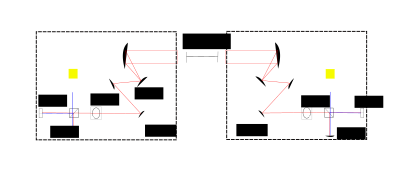
\includegraphics[scale=.3]{movable_app}}
	\caption{Incoming beam (red) passes a movable aperture and interferes with local beam (blue).}
	\label{fig:4}
	\end{figure}



\sectionend

\section{Tophat-Gaussian Interference: FIRST ITERATION}

This chapter is largely deprecated as it makes less stringent approximations than the chapter that follows. However, it makes use of a more formal Taylor (Maclaurin) series expansion which can serve as a check for the following chapter.

\subsection{Tophat Representation as Superposition of HG modes}

Tophat mode coefficients in a given basis can be constructed by...

\clearpage

\subsection{First-order Shifting and Tilting Tophat}

In shifting and tilting the tophat (to first order), we gain from the exponential terms in HG modes

\begin{align*}
\sum u_{nm} \rightarrow_{shift,tilt} &
    \sum u_{nm}' \left[
        1+ i k \alpha x
    \right]
\end{align*}


where the second term arises from tilting exponential terms in HG modes. The new modes $u_{nm}'$ are functions of $H_n(\frac{\sqrt{2}(x+a)}{w(z)})$, resulting from the unidirectional shift $x+a$. To first order, the new modes resulting from this shift follow

\begin{align*}
	u_{nm}' =& u_{nm} + a \frac{\partial u_{nm}}{\partial x}
	\\=&
		u_{nm} 
		-
		\frac{2ax}{w(z)^2} 
		u_{nm}
		\\&+
		(2^{n+m-1}n!m!\pi)^{-1/2}
		\frac{1}{w(z)}
		H_{m} \Big(\frac{\sqrt{2}y}{w(z)} \Big)
		\exp \Big(\frac{-ik(x^{2}+y^{2})}{2R_{c}(z)}-
		\frac{x^{2}+y^{2}}{w(z)^{2}} 
		+i(n+m+1)(\Psi(z))		
		\Big)\;
		\times
		a 		
		\frac{\partial H_n(\frac{\sqrt{2}x }{w(z)})}{\partial x}
			\\=&
		u_{nm}
		[
		1
		-
		\frac{2ax}{w(z)^2}]		
		+
		a 	
		u_{nm}(	
		\frac{\partial H_n(\frac{\sqrt{2}x }{w(z)})}{\partial x}
		)
		.
\end{align*}

Where the last term is $u_{nm}$ as a function of $H_n'$. Derivative of Hermite polynomials:


\begin{equation*}
	H_n'(x) = 2n H_{n-1} (x)
\end{equation*}

Therefore

\begin{align*}
	\frac{\partial H_n(\frac{\sqrt{2}x }{w(z)})}{\partial x}
	=&
	\frac{2 \sqrt{2} n}{w(z)} H_{n-1}\Big(\frac{\sqrt{2}x}{w(z)}\Big)
\end{align*}

so that the tophat is now expressed as

\begin{align*}
	\sum u_{nm} \rightarrow_{shift,tilt}&
    \left[
    u_{nm} 
    [
		1
		-
		\frac{2ax}{w(z)^2}]	
	+ 
	a \frac{2 \sqrt{2} n}{w(z)} 
	u_{nm}(H_{n-1}) \right]
	\left[
        1+ i k \alpha x
    \right]
    \\=&
     u_{nm}
        \left[
        1 - \frac{2 a }{w(z)^2} x + i k \alpha x - i \frac{2 k \alpha a}{w(z)^2} x^2 
    \right]
    + 
	a \frac{2 \sqrt{2} n}{w(z)} 
	u_{nm}(H_{n-1})
	\left[
        1+ i k \alpha x
    \right]
\end{align*}

where $u_{nm} (H_{n-1})$ can be rewritten

\begin{align*}
	u_{nm} (H_{n-1}) =&
	(\frac{2 n }{2 n})^{1/2}
			\exp(-i \Psi(z))\exp(i \Psi(z))
			\\& \times
	[
	(2^{n+m-1}n!m!\pi)^{-1/2}
		\frac{1}{w(z)}
		H_{n-1} \Big(\frac{\sqrt{2}x}{w(z)} \Big)
		H_{m} \Big(\frac{\sqrt{2}y}{w(z)} \Big)
	\\& \times		
		\exp \Big(\frac{-ik(x^{2}+y^{2})}{2R_{c}(z)}-
		\frac{x^{2}+y^{2}}{w(z)^{2}} 
		+i(n+m+1)\Psi(z)		
		\Big)
				]
		\\=&
		(\frac{1}{2 n}) ^{1/2}
		\exp(i \Psi(z))
			(2^{(n-1)+m-1}(n-1)!m!\pi)^{-1/2}
		\frac{1}{w(z)}
		H_{n-1} \Big(\frac{\sqrt{2}x}{w(z)} \Big)
		H_{m} \Big(\frac{\sqrt{2}y}{w(z)} \Big)
			\\& \times	
		\exp \Big(\frac{-ik(x^{2}+y^{2})}{2R_{c}(z)}-
		\frac{x^{2}+y^{2}}{w(z)^{2}} 
		+i( (n-1)+m+1)\Psi(z)			
		\Big)
		\\=&
		\sqrt{\frac{1}{2 n}}
		\exp(i \Psi(z))
		u_{n-1,m}
\end{align*}

The new tophat modes after applying first-order shift ($x+a$) and tilt are 

\begin{equation}\label{eq:prev}
	u_{n,m} \rightarrow
     u_{n,m}
        \left[
        1 - \frac{2 a }{w(z)^2} x + i k \alpha x - i \frac{2 k \alpha a}{w(z)^2} x^2 
    \right]
    + 
	a \frac{2 \sqrt{n}}{w(z)} 
	\exp(i \Psi(z))
	u_{n-1,m}
	\left[
        1+ i k \alpha x
    \right]	 \; .
\end{equation}

Rewriting this result using the general scattering equations (Eq. \ref{scatter_x} and Eq. \ref{scatter_x2}):

\begin{align*}
\sum_{n,m} u_{n,m} \rightarrow 
	\sum_{n,m} 
	\lbrace &
		u_{n+2,m} [\frac{w^2}{4}(1-i \frac{z}{z_R})^2 \sqrt{(n+1)(n+2)} ][-i\frac{2ka\alpha}{w^2}]
		\\+&
		u_{n+1,m} [\frac{w}{2}(1-i\frac{z}{z_R})\sqrt{n+1}][ik\alpha - \frac{2a}{w^2}]
		\\+&
		u_{n,m} [1+\frac{w}{2}(1-i\frac{z}{z_R})\sqrt{n+1})[ik\alpha \frac{2a\sqrt{n}}{w} exp(i \Psi(z))]]
		\\+&
		u_{n-1,m} [\frac{2a\sqrt{n}}{w} + \frac{w}{2}(\sqrt{n}(1+i\frac{z}{z_R}))[ik\alpha - \frac{2a}{w^2}]]
		\\+&
		u_{n-2,m} [ikan\alpha(1+i\frac{z}{z_R}) - i\frac{ka\alpha}{2}
(1-i\frac{z}{z_R})^2 \sqrt{n(n-1)}		
		] 	
	\rbrace
\end{align*}

Rewriting for scattering factors:

\begin{align*}
\sum_{n,m} u_{n,m} \rightarrow 
	\sum_{n,m} 
	\lbrace &
		u_{n+2,m}[ X_+^2(-i\frac{2ka\alpha}{w^2})]
		\\+&
		u_{n+1,m}[ X_+^1(ik\alpha - \frac{2a}{w^2})]
		\\+&
		u_{n,m} [1+X_+^1(ik\alpha \frac{2a\sqrt{n}}{w} e^{i\Psi})- X_0^2 (i\frac{2ka\alpha}{w^2})]
		\\+&
		u_{n-1,m} [\frac{2a\sqrt{n}}{w} e^{i\Psi} + X_-^1(ik\alpha - \frac{2a}{w^2})]
		\\+&
		u_{n-2,m} [ X_-^1(ik\alpha a\frac{2\sqrt{n}}{w}e^{i\Psi}) - X_-^2 (i\frac{2ka\alpha}{w^2})] 	
	\rbrace
\end{align*}

\clearpage

\subsection{Second-order Shift, First-order Tilt Tophat}

To second order in shift, gain an additional

\begin{align*}
	\frac{a^2}{2} (\frac{\partial^2 u_{nm}}{\partial x^2}) [1+ik\alpha x] =&
	\frac{a^2}{2} [1+ik\alpha x] [-\frac{2}{w^2}u_{nm} + (\frac{2x}{w^2})^2 u_{nm} - \frac{4x}{w^2}u_{nm}' + u_{nm}'']
\end{align*}

Where $u_{nm}'=	\frac{2 \sqrt{n}}{w(z)} 
	\exp(i \Psi(z))
	u_{n-1,m}$ represents $u_{nm}$ as a function of $H_n'$. Similarly, for $u_{nm}''$

\begin{equation}
	H_n^c= 2^c\frac{n!}{(n-c)!}H_{n-c}
\end{equation}

\begin{align*}
	H_n''(\frac{\sqrt{2}x}{w}) = 
	\frac{8}{w^2} \frac{n!}{(n-2)!}H_{n-2}
	\\=&
	\frac{8}{w^2} (n(n-1)) H_{n-2}
\end{align*}

And rewrite

\begin{equation*}
	u_{nm} (H_{n-2}) = \sqrt{\frac{1}{4 n(n-1)}}
		\exp(2i \Psi)
		u_{n-2,m}
\end{equation*}

Then

\begin{align*}
\frac{a^2}{2} [1+ik\alpha x] [-\frac{2}{w^2}u_{nm} + (\frac{2x}{w^2})^2 u_{nm} - \frac{4x}{w^2}u_{nm}' + u_{nm}'']
=&
\frac{a^2}{2} [1+ik\alpha x]
\\ \times&
[(\frac{4x^2-2w^2}{w^4}) u_{nm} 
\\-& \frac{8x \sqrt{n}}{w^3}
	\exp(i \Psi)
	u_{n-1,m}
\\+& 
	\frac{4}{w^2}
	\sqrt{n(n-1)}
		\exp(2i \Psi)
		u_{n-2,m}]
		\\=&
		C
\end{align*}

distributing,

\begin{align*}
C =&
\frac{a^2}{2} 
\\ \times&\{
[( \frac{4x^2}{w^2} -\frac{2}{w^2} )u_{nm} 
- \frac{8x \sqrt{n}}{w^3}
	\exp(i \Psi)
	u_{n-1,m}
+
	\frac{4}{w^2}
	\sqrt{n(n-1)}
		\exp(2i \Psi)
		u_{n-2,m}]
	\\+&
	ik \alpha
	[( \frac{4x^3}{w^2} -\frac{2x}{w^2} )u_{nm} 
- \frac{8x^2 \sqrt{n}}{w^3}
	\exp(i \Psi)
	u_{n-1,m}
+ 
	\frac{4x}{w^2}
	\sqrt{n(n-1)}
		\exp(2i \Psi)
		u_{n-2,m}]
		\}
\end{align*}

In terms of the higher-order HG mode coupling coefficients, this adds to the first-order solution:



\clearpage

\subsection{First-order Shift, Second-order Tilt Tophat}

Using results of the previous section, a second-order tilt would yield

\begin{align*}
	\sum u_{nm} \rightarrow_{shift,tilt}&
    \left[
    u_{nm} 
    [
		1
		-
		\frac{2ax}{w(z)^2}]	
	+ 
	a \frac{2 \sqrt{2} n}{w(z)} 
	u_{nm}(H_{n-1}) \right]
	\left[
        1+ i k \alpha x - \frac{1}{2}(\alpha k x)^2
    \right]
    \\=&
     u_{nm}
        \left[
        1 - \frac{2 a }{w(z)^2} x + i k \alpha x - i \frac{2 k \alpha a}{w(z)^2} x^2 
        -\frac{1}{2}(\alpha k)^2 x^2 + 
        \frac{a(\alpha k)^2}{w(z)^2}x^3
    \right]
    \\+& 
	a \frac{2 \sqrt{2} n}{w(z)} 
	u_{nm}(H_{n-1})
	\left[
        1+ i k \alpha x - \frac{1}{2}(\alpha k)^2 x^2
    \right].
\end{align*}

Solving the $u_{nm}(H_{n-1})$ terms,

\begin{align*}
	u_{n,m} \rightarrow &
	     u_{nm}
        \left[
        1 - \frac{2 a }{w(z)^2} x + i k \alpha x - i \frac{2 k \alpha a}{w(z)^2} x^2 
        -\frac{1}{2}(\alpha k)^2 x^2 + 
        \frac{a(\alpha k)^2}{w(z)^2}x^3
    \right]
    \\+& 
	a \frac{2 \sqrt{n}}{w(z)} 
	\exp(i \Psi(z))
	u_{n-1,m}
	\left[
        1+ i k \alpha x - \frac{1}{2}(\alpha k)^2 x^2
    \right]	 \; .
\end{align*}

\clearpage

\subsection{Tophat Change of Basis (AW) }

No we seek a solution applied to the previous subsection for interference with the shift-tilted tophat with a Gaussian beam. 
Where $\gamma \in \{0,1,2\}$, representing scattered modes in the previous subsection, $(a,b) = (n\pm \gamma,m)$

\begin{equation*}
	\int_{-Y}^{Y}dy \int_{x_1}^{x_2}
	dx \; HG_{0,0}^*HG_{a,b}
\end{equation*}

also represented as

\begin{equation*}
	\langle 0,0 | a,b \rangle
\end{equation*}

This goes to 

\begin{align*}
	\langle 0,0 | a,b \rangle
	\rightarrow &
	\frac
	{
		2^{a+b+1}
		\sqrt{a!b!}
		e^{i(\Delta w t 
		- (k_2 Z - k_1d_1)
		)}
	}
	{
		\pi \sqrt{\sigma_x \sigma_y^{1+b}}
		w_1 w_2^{1+a+b}
		(1+i \frac{d_1}{z_r1})
		(1-i \frac{Z}{z_r2})^{1+a+b}
	}
	\\& \times
	\sum_{A=0}^{\lfloor{\frac{a}{2}} \rfloor}
	\sum_{B=0}^{\lfloor{\frac{b}{2}} \rfloor}
	\frac
	{
		-\frac{1}{8}^{A+B}
		W_2^{2(A+B)}
		\sigma_y^B		
	}
	{
		A!B!(b-2B)!
	}
	\\& \times
	[
		G(\sqrt{\sigma}Y;b-2B)
		-
		G(-\sqrt{\sigma}Y;b-2B)		
	]
	\\& \times
	\frac{1}{(a-2A)!\sigma^{\frac{a}{2}-A}}
	\\& \times
	[
		G(\sqrt{\sigma}x_2;a-2A)
		-
		G(\sqrt{\sigma}x_1;a-2A)			
	]
\end{align*}

which is equivalent to 

\begin{align*}
 \langle 0,0 | a,b \rangle =&
 	\frac
 	{
 		2^{a+b+1}
 		\sqrt{a!b!}
 		e^{i(\Delta w t 
			- (k_2 Z - k_1d_1)
		)}
 	}
 	{
 		\pi \sqrt{\sigma^{2+a+b}}
 		w_1 w_2^{1+a+b}
 		(1+i \frac{d_1}{z_{r1}})
 		(1-i \frac{Z}{z_{r2}})^{1+a+b}	
 	}
 	\\& \times
		\sum_{A=0}^{\lfloor{\frac{a}{2}} \rfloor}
		\sum_{B=0}^{\lfloor{\frac{b}{2}} \rfloor}
		\frac
		{
			(-\frac{\sigma}{8})^{A+B}
			W_2^{2(A+B)}	
		}
		{
			A!B! (a-2A)!(b-2B)!
		}
 	\\& \times
 		[
		G(\sqrt{\sigma}Y;b-2B)
		-
		G(-\sqrt{\sigma}Y;b-2B)		
	]
	[
		G(\sqrt{\sigma}x_2;a-2A)
		-
		G(\sqrt{\sigma}x_1;a-2A)			
	]
\end{align*}

The $G$ functions have symmetry in the $y$ case

\begin{equation*}
	G(-x;T) = -G(x;T)
\end{equation*}

for even $T$ and 

\begin{equation*}
	G(-x;T) = G(x;T)
\end{equation*}

for odd $T$. So $ 		[
		G(\sqrt{\sigma}Y;b-2B)
		-
		G(-\sqrt{\sigma}Y;b-2B)		
	]$ is 0 if $b$ odd and if $2G(\sqrt{\sigma}Y;b-2B)$ is even.\\ 
Therefore, for odd $b$:

\begin{equation*}
	\langle a,b| 0,0 \rangle=0
\end{equation*}

for even $b$:

\begin{align*}
 \langle 0,0 | a,b \rangle =&
 	\frac
 	{
 		2^{a+b+1}
 		\sqrt{a!b!}
 		e^{i(\Delta w t 
			- (k_2 Z - k_1d_1)
		)}
 	}
 	{
 		\pi \sqrt{\sigma^{2+a+b}}
 		w_1 w_2^{1+a+b}
 		(1+i \frac{d_1}{z_{r1}})
 		(1-i \frac{Z}{z_{r2}})^{1+a+b}	
 	}
 		\\& \times
			\sum_{A=0}^{\lfloor{\frac{a}{2}} \rfloor}
			\sum_{B=0}^{\lfloor{\frac{b}{2}} \rfloor}
			\frac
			{
				(-\frac{\sigma}{8})^{A+B}
				W_2^{2(A+B)}
				\Gamma(\frac{b+1}{2}-B)		
			}
			{
				A!B!(a-2A)!(b-2B)!
			}
		\\& \times
			[
				\mathrm{erf}(\sqrt{\sigma}Y)
				-
				\frac{2e^{-\sigma Y^2}}{\sqrt{\pi}}
				\sum_{M=0}^{\frac{b}{2}-(B+1)}
				\frac{(M+1)!}{(2(M+1))!}
				(2\sqrt{\sigma}Y)^{2M+1}
			]
		\\& \times
			[
				G(\sqrt{\sigma}x_2;a-2A)
				-
				G(\sqrt{\sigma}x_1;a-2A)			
			]
\end{align*}

For the functions

\begin{equation*}
	G(x;m) = \frac{m!}{2^m (\frac{m}{2})!}
	[
		\sqrt{\pi}\frac{erf(x)}{2}
		-
		\frac{e^{-x^2}}{\pi}
		\sum_{M=0}^{\frac{m}{2}-1}
		\frac{(M+1)!}{(2(M+1))!} (2x)^{2M+1}	
	]
\end{equation*}

This can be rewritten, for even $m$:

\begin{equation*}
	G(x;m) = \Gamma(\frac{m+1}{2})
	[
		\frac{erf(x)}{2}
		-
		\frac{e^{-x^2}}{\pi}
		\sum_{M=0}^{\frac{m}{2}-1}
		\frac{(M+1)!}{(2(M+1))!} (2x)^{2M+1}	
	]
\end{equation*}

and for odd $m$:

\begin{equation*}
	G(x;m) = 
		-\frac{(\frac{m-1}{2})! e^{-x^2}}{2}
		\sum_{M=0}^{\frac{m-1}{2}} \frac{x^{2M}}{M!}
\end{equation*}

and $\sigma$ is defined as

\begin{equation}
	\sigma = 
		\frac{1}{w_1^2 (1+i\frac{d_1}{z_{r1}})}
		+
		\frac{1}{w_2^2 (1-i\frac{Z}{z_{r2}})}			
\end{equation}

\sectionend

\subsection{COR Aperture: First-order Shifting and Tilting Tophat}

 To first order, the new modes resulting from a shift ($x+a$) follow

\begin{align*}
	u_{nm}' =& u_{nm}(x)|_{a=0} + a (\frac{\partial u_{nm}(x)}{\partial x})_{a=0}
	\\=&
		u_{nm} 
		-
		\frac{2ax}{w(z)^2} 
		u_{nm}
		\\&+
		(2^{n+m-1}n!m!\pi)^{-1/2}
		\frac{1}{w(z)}
		H_{m} \Big(\frac{\sqrt{2}y}{w(z)} \Big)
		\exp \Big(\frac{-ik(x^{2}+y^{2})}{2R_{c}(z)}-
		\frac{x^{2}+y^{2}}{w(z)^{2}} 
		+i(n+m+1)(\Psi(z))		
		\Big)\;
		\times
		a 		
		\frac{\partial H_n(\frac{\sqrt{2}x }{w(z)})}{\partial x}
			\\=&
		u_{nm}
		[
		1
		-
		\frac{2ax}{w(z)^2}]		
		+
		a 	
		u_{nm}(	
		\frac{\partial H_n(\frac{\sqrt{2}x }{w(z)})}{\partial x}
		)
		.
\end{align*}

Where the last term is $u_{nm}$ as a function of $H_n'$. Derivative of Hermite polynomials:


\begin{equation*}
	H_n'(x) = 2n H_{n-1} (x)
\end{equation*}

Therefore

\begin{align*}
	\frac{\partial H_n(\frac{\sqrt{2}x }{w(z)})}{\partial x}
	=&
	\frac{2 \sqrt{2} n}{w(z)} H_{n-1}\Big(\frac{\sqrt{2}x}{w(z)}\Big)
\end{align*}

so that the tophat is now expressed as

\begin{align*}
	\sum u_{nm} \rightarrow_{shift}&    
     u_{nm}
        \left[
        1 - \frac{2 a }{w(z)^2} x 
    \right]
    + 
	a \frac{2 \sqrt{2} n}{w(z)} 
	u_{nm}(H_{n-1})
\end{align*}

where $u_{nm} (H_{n-1})$ can be rewritten

\begin{align*}
	u_{nm} (H_{n-1}) =&
	(\frac{2 n }{2 n})^{1/2}
			\exp(-i \Psi(z))\exp(i \Psi(z))
			\\& \times
	[
	(2^{n+m-1}n!m!\pi)^{-1/2}
		\frac{1}{w(z)}
		H_{n-1} \Big(\frac{\sqrt{2}x}{w(z)} \Big)
		H_{m} \Big(\frac{\sqrt{2}y}{w(z)} \Big)
	\\& \times		
		\exp \Big(\frac{-ik(x^{2}+y^{2})}{2R_{c}(z)}-
		\frac{x^{2}+y^{2}}{w(z)^{2}} 
		+i(n+m+1)\Psi(z)		
		\Big)
				]
		\\=&
		(\frac{1}{2 n}) ^{1/2}
		\exp(i \Psi(z))
			(2^{(n-1)+m-1}(n-1)!m!\pi)^{-1/2}
		\frac{1}{w(z)}
		H_{n-1} \Big(\frac{\sqrt{2}x}{w(z)} \Big)
		H_{m} \Big(\frac{\sqrt{2}y}{w(z)} \Big)
			\\& \times	
		\exp \Big(\frac{-ik(x^{2}+y^{2})}{2R_{c}(z)}-
		\frac{x^{2}+y^{2}}{w(z)^{2}} 
		+i( (n-1)+m+1)\Psi(z)			
		\Big)
		\\=&
		\sqrt{\frac{1}{2 n}}
		\exp(i \Psi(z))
		u_{n-1,m}
\end{align*}

The new tophat mode coefficients after applying the  first-order shift ($x+a$) are 

\begin{equation}
	u_{n,m} \rightarrow
     u_{n,m}
        \left[
        1 - \frac{2 a }{w(z)^2} x 
    \right]
    + 
	a \frac{2 \sqrt{n}}{w(z)} 
	\exp(i \Psi(z))
	u_{n-1,m} \; .
\end{equation}

For rotation about the aperture (neglecting the shift), apply a rotation matrix to the coordinates of interest:

\begin{align*}
\begin{pmatrix}
x' \\
z'
\end{pmatrix} 
=&
\begin{pmatrix}
x \\
z
\end{pmatrix} 
\begin{pmatrix}
\cos\alpha & \sin\alpha \\
-\sin\alpha & \cos\alpha
\end{pmatrix}
\\ \approx &
	\begin{pmatrix}
x+z\alpha \\
z - x\alpha
\end{pmatrix}
\end{align*}

For rotation with respect to the shifted beam (at the aperture along the optical axis, $z=0$, at a point $a$-shifted in $x$):
 \begin{align*}
\begin{pmatrix}
x' \\
z'
\end{pmatrix} 
=&
	\begin{pmatrix}
(x+a)+z\alpha \\
z - (x+a)\alpha
\end{pmatrix}
 \end{align*}

The new modes after rotation  about the shifted beam are approximately, where $u_{nm}$ is a function of $H_{n}^{'}=H_n(\sqrt{2}x/w(z))$, $e^{-x'^2/w^2}$ and $e^{-ikz'}$:

\begin{align*}
	u_{nm} \rightarrow&
	u_{nm} (H_{n}^{'}, e^{-ikz'},e^{-x'^2/w^2})
	\\=&
		(H_{n} \Big(\frac{\sqrt{2}[x+z\alpha]}{w} \Big) e^{-ik[z-x\alpha]} e^{-[x^2 + (z\alpha)^2+ 2xz\alpha}])
		\\ \times&
		[
		(2^{n+m-1}n!m!\pi)^{-1/2}
		\frac{1}{w}
		H_{m} \Big(\frac{\sqrt{2}y}{w} \Big)
		\exp \Big(\frac{-ik(x^{2}+y^{2})}{2R_{c}}-
		\frac{x^{2}+y^{2}}{w^{2}} 
		+i(n+m+1)(\Psi)		
		\Big)
		]\;
			\\=&
	u_{nm}(H_{n}^{'}, \exp[ikx\alpha -z^2\alpha^2 - 2xz\alpha])
	\\ \approx &
	u_{nm} + \alpha u_{nm}[ \frac{\partial  H_{n}^{'} }{\partial\alpha}   + \frac{\partial e^{ikx\alpha-z^2\alpha^2 - 2xz\alpha}}{\partial \alpha} ]_{\alpha=0}
\end{align*}

Also, accounting for the $u_{n-1,m}$ term from the shift

\begin{align*}
	u_{nm} \rightarrow&
	u_{n-1,m} (H_{n-1}^{'}, e^{ikx\alpha-z^2\alpha^2 - 2xz\alpha})
	\\ \approx &
	u_{n-1,m} + \alpha u_{n-1,m}[ \frac{\partial  H_{n-1}^{'} }{\partial\alpha}   + \frac{\partial e^{ikx\alpha-z^2\alpha^2 - 2xz\alpha}}{\partial \alpha} ]_{\alpha=0}
\end{align*}

The last term gives the usual $ik\alpha x$ with additional terms

\begin{align*}
	\alpha u_{nm}[\frac{\partial e^{ikx\alpha-z^2\alpha^2 - 2xz\alpha}}{\partial \alpha}]_{\alpha=0}
	=&
	\alpha u_{nm}[ikx e^{ikx\alpha-z^2\alpha^2 - 2xz\alpha}]_{\alpha=0}
	\\=& \alpha u_{nm} [e^{ikx\alpha-z^2\alpha^2 - 2xz\alpha}(ikx-(2 z^2\alpha + 2xz)/w^2)]_{\alpha=0}
	\\=&
	\alpha u_{nm} [ikx- \frac{2xz}{w^2}]
\end{align*}

The Hermite polynomial differentiation goes as

\begin{align*}
	[\frac{\partial H_n(\frac{\sqrt{2}(x+\alpha) }{w(z)})}{\partial x}]_{\alpha=0}
	=&
	\frac{2 \sqrt{2} n}{w(z)} H_{n-1}\Big(\frac{\sqrt{2}x}{w(z)}\Big)
\end{align*}

or (for the $u_{n-1,m}$ term from the shift)

\begin{align*}
	[\frac{\partial H_{n-1}(\frac{\sqrt{2}(x+\alpha) }{w(z)})}{\partial x}]_{\alpha=0}
	=&
	\frac{2 \sqrt{2} (n-1)}{w(z)} H_{n-1}\Big(\frac{\sqrt{2}x}{w(z)}\Big)
\end{align*}

\section{Approximations to Tophat-Gaussian Interference}

\subsection{First-order Shifting Tophat}

 To first order, the new modes resulting from a shift ($x' = x+a$), making the coordinate change in three primed terms of interest, follow ($w=w(z)$ and $R_c=R_c(z)$):

\begin{align*}
	u_{nm} \rightarrow
		(2^{n+m-1}n!m!\pi)^{-1/2}
		\frac{1}{w}
		H_{n} \Big(\frac{\sqrt{2}x'}{w} \Big)
		H_{m} \Big(\frac{\sqrt{2}y}{w} \Big)
		\exp \Big(\frac{-ik(x'^{2}+y^{2})}{2R_{c}}-
		\frac{x'^{2}+y^{2}}{w^{2}} 
		+i(n+m+1)\Psi - ikz
		\Big)\;
		.
\end{align*}

For small shift in the exponential term

\begin{align*}
\exp( -\frac{(x+a)^2}{w^2})
=&
	\exp( -\frac{x^2+2ax+a^2}{w^2})
	\\=&
	\exp( -\frac{x^2}{w^2})\exp( -\frac{2ax+a^2}{w^2})
	\\ \approx &
	\exp( -\frac{x^2}{w^2})\exp( -\frac{2ax}{w^2})	\;,(1st-order)
	\\ \approx &
	\exp( -\frac{x^2}{w^2})( 1-\frac{2ax}{w^2})
\end{align*}

Likewise, for the curvature term

\begin{align*}
\exp \Big(\frac{-ik( (x+a)^{2}+y^{2}}{2R_{c}} \Big)
 \approx &
	\exp( -ik\frac{x^2+y^2}{2 R_c})
	( 1-\frac{2ikax}{2R_c}
	-\frac{ika^2}{2R_c})
	\\ \approx &
	\exp( -ik\frac{x^2+y^2}{2 R_c})
	( 1-\frac{ikax}{R_c})\;,(1st-order)
\end{align*}

These two results leave the new mode, save for the shifted $H_n$ term,

\begin{align*}
	u_{nm} \rightarrow u_{nm}( 1-\frac{2ax}{w^2})
	( 1-\frac{ikax}{R_c})
\end{align*}

To first order then,

\begin{align*}
	u_{nm} \rightarrow u_{nm}( 1-\frac{2ax}{w^2}-\frac{ikax}{R_c})
\end{align*}

\rule{\textwidth}{0.4pt}

For $H_n(\frac{\sqrt{2} (x+a) }{w})$, use the identity

\begin{align*}
	H_n(X+Y) = (H(X)+2Y)^n,
\end{align*}

where $H^n = H_n$ in this case. For the shifted polynomial, let $X \equiv \frac{\sqrt{2}x}{w}$ and $Y \equiv \frac{\sqrt{2}a}{w}$. 

Examples using the identity (note, $H_0$ is always $1$):\\

\[
  H_{n}(X+Y)=\begin{cases}
               1 \tab\tab\tab\tab\tab\;\;(n=0)\\
               H_1(X) + 2Y \tab\tab\tab\tab\;\;\;(n=1)\\
               H_2(X) + 2(2Y)H_1(X) + (2Y)^2 \tab\tab\;\;(n=2)\\
               H_3(X) + 3(2Y)H_2(X) +3(2Y)^2H_1(X)+(2Y)^3\tab\;\;(n=3)
            \end{cases}
\]

As a simple check let $X = Y = 1$ for the $n=3$ case, the result using the identity and solving the corresponding polynomials is

\begin{align*}
	H_3 (X+Y) =&
	(8-12)
	+ 3(2)(4-2)
	+ 3(2)^2(2)
	+ (2)^3
	\\=&
	-4 + 12 + 24 + 8
	\\=&
	40
\end{align*}

Without the identity, the solution matches:

\begin{align*}
	H_3 (1+1) = H_3(2) =&
	8(2)^3 - 12(2)
	\\=& 40
\end{align*}

Now to generalize by inspection. The $Y$ term is linear in shift, and it is always the second term in the identity, with a factor of binomial coefficient and $H_{n-1}$. The first-order expansion then only needs account for the binomial coefficient for $n-1$, given by ${n\choose 1} = \frac{n!}{(n-1)!}=n$. Therefore, the first-order term from the shifted hermite polynomial is 

\begin{align*}
	H_n(\frac{\sqrt{2}(x+a)}{w}) \approx&
	 H_n(\frac{\sqrt{2}x}{w})+ 
	 	 \frac{2\sqrt{2}n a}{w}
	 	 H_{n-1}(\frac{\sqrt{2}x}{w}).
\end{align*}

In summary, this term yielded

\begin{align*}
u_{nm} \rightarrow u_{nm} + \frac{2\sqrt{2}n a}{w}
	 	 H_{n-1}(\frac{\sqrt{2}x}{w}) u_{nm}' 
\end{align*}

where $u_{nm}'$ includes no $H_n$. The $u_{nm}'$ term with the $H_{n-1}$ factor can be viewed as $u_{nm}$ as a function of $H_{n-1}$. This is cumbersome, since the goal is to solve for on-axis mode coefficients. However, the combination can be rewritten as a single $u_{n-1,m}$ mode with an additional factor by shifting in $n$:

\begin{align*}
	u_{nm} (H_{n-1}) =&
	(\frac{2 n }{2 n})^{1/2}
			\exp(-i \Psi(z))\exp(i \Psi(z))
			\\& \times
	[
	(2^{n+m-1}n!m!\pi)^{-1/2}
		\frac{1}{w(z)}
		H_{n-1} \Big(\frac{\sqrt{2}x}{w(z)} \Big)
		H_{m} \Big(\frac{\sqrt{2}y}{w(z)} \Big)
	\\& \times		
		\exp \Big(\frac{-ik(x^{2}+y^{2})}{2R_{c}(z)}-
		\frac{x^{2}+y^{2}}{w(z)^{2}} 
		+i(n+m+1)\Psi(z)		
		\Big)
				]
		\\=&
		(\frac{1}{2 n}) ^{1/2}
		\exp(i \Psi(z))
			(2^{(n-1)+m-1}(n-1)!m!\pi)^{-1/2}
		\frac{1}{w(z)}
		H_{n-1} \Big(\frac{\sqrt{2}x}{w(z)} \Big)
		H_{m} \Big(\frac{\sqrt{2}y}{w(z)} \Big)
			\\& \times	
		\exp \Big(\frac{-ik(x^{2}+y^{2})}{2R_{c}(z)}-
		\frac{x^{2}+y^{2}}{w(z)^{2}} 
		+i( (n-1)+m+1)\Psi(z)			
		\Big)
		\\=&
		\sqrt{\frac{1}{2 n}}
		\exp(i \Psi(z))
		u_{n-1,m}
\end{align*}

This leaves

\begin{align*}
u_{nm} \rightarrow
u_{nm} + 
	a \frac{2 \sqrt{n}}{w} 
	\exp(i \Psi)
	u_{n-1,m} \; .
\end{align*}

\rule{\textwidth}{0.4pt}

The new tophat mode coefficients after applying the  first-order shift ($x+a$) are 

\begin{align*}
	u_{n,m} \rightarrow
	\left[
     u_{n,m}
    + 
	a \frac{2 \sqrt{n}}{w(z)} 
	\exp(i \Psi(z))
	u_{n-1,m}
	\right]
	 \left[
        1 - \frac{2 a }{w^2} x 
    \right] 
	\left[ 1-\frac{2ax}{2R_c}
	\right]    
    \; .
\end{align*}

To first order in $a$, neglect factoring the second terms in all braces. This leaves

\begin{align*}
	u_{n,m} \rightarrow
     u_{n,m}
     	 \left[
        1 - a\frac{2 x}{w^2}  
        - a \frac{ikx}{R_c}
    \right]
    + 
	a \frac{2 \sqrt{n}}{w(z)} 
	\exp(i \Psi)
	u_{n-1,m} \; .
\end{align*}

\subsection{First-order tilting tophat (without propagation)}

For rotation about the aperture (neglecting the shift), apply a rotation matrix to the coordinates of interest:

\begin{align*}
\begin{pmatrix}
x' \\
z'
\end{pmatrix} 
=&
\begin{pmatrix}
x \\
z
\end{pmatrix} 
\begin{pmatrix}
\cos\alpha & \sin\alpha \\
-\sin\alpha & \cos\alpha
\end{pmatrix}
\\ \approx &
	\begin{pmatrix}
x+z\alpha \\
z - x\alpha
\end{pmatrix}
\end{align*}


The new modes $u_{nm}$ after rotation  about the aperture, again priming three transformed coordinates of interest, follow

\begin{align*}
	u_{nm} \rightarrow
		(2^{n+m-1}n!m!\pi)^{-1/2}
		\frac{1}{w}
		H_{n} \Big(\frac{\sqrt{2}x'}{w} \Big)
		H_{m} \Big(\frac{\sqrt{2}y}{w} \Big)
		\exp \Big(\frac{-ik(x^{2}+y^{2})}{2R_{c}}-
		\frac{x'^{2}+y^{2}}{w^{2}} 
		+i(n+m+1)\Psi(z') - ikz'		
		\Big)\;
		.
\end{align*}

\rule{\textwidth}{0.4pt}

Approximation to first order of the tilted exponential term in $z'$ for the wave term

\begin{align*}
	\exp(-ik(z-x\alpha )) =&
	\exp(-ikz)\exp(ikx\alpha )
	\\ \approx &
	\exp(-ikz)(1+ikx\alpha)
\end{align*}

This approximation results in

\begin{align*}
	u_{nm} \rightarrow
	u_{nm}[1+ikx\alpha ]
\end{align*}

For $H_n$ tilted, results of the shift approximation go as $x \rightarrow z \alpha$:

\begin{align*}
u_{nm} \rightarrow
u_{nm} + 
	z \alpha \frac{2 \sqrt{n}}{w} 
	\exp(i \Psi)
	u_{n-1,m} \; .
\end{align*}

\rule{\textwidth}{0.4pt}

For the Gouy phase term,

\begin{align*}
	\exp(i(N+1)\Psi(z' )) =&
	\exp[i(N+1)\arctan(\frac{z-x\alpha}{z_R})]
	\\ \approx &
	\exp[i(N+1) (
	\arctan(\frac{z}{z_R})
	-\frac{z_R x\alpha}{z^2 + z_R^2}
	)
	]
		\\ \approx &
	\exp[i(N+1)(
	\Psi(z) 
	-\frac{z_R x\alpha}{z^2 + z_R^2}
	)
	]
			\\ \approx &
	\exp[i(N+1)\Psi(z)] 
	\times i(N+1)
	(1 - \frac{z_R x\alpha}{z^2 + z_R^2})
\end{align*}

the result is then

\begin{align*}
	u_{nm} \rightarrow
	u_{nm}[1 - i(N+1)
	\frac{z_R x\alpha}{z^2 + z_R^2}]
\end{align*}

where $N=n+m$.

\rule{\textwidth}{0.4pt}

Altogether, the rotation yields (to first order in $\alpha$)

\begin{align*}
	u_{nm} \rightarrow
	u_{nm}[1 + ikx\alpha 
	- i(N+1)
	\frac{z_R x\alpha}{z^2 + z_R^2}]
\end{align*}

\subsection{First-order shifted,tilted tophat (without propagation)}

Tilting the shifted beam then yields (where $w=w(z)$, and $\phi \equiv \exp(i\Psi)$, $\eta = (N+1)
	\frac{z_R}{z^2 + z_R^2})$

\begin{align*}
	     u_{n,m}
     	 \left[
        1 - a\frac{2 x}{w^2}  
        - a \frac{ikx}{R_c}
    \right]
    + 
	a \frac{2 \sqrt{n}}{w} 
	\phi
	u_{n-1,m} \rightarrow&
	     u_{n,m}
	     [1
	     +ikx\alpha
	     - i\alpha x \eta
	     ]
     	 \left[
        1 - a\frac{2 x}{w^2}  
        - a \frac{ikx}{R_c}
    \right]
    \\ & + 
	a \frac{2 \sqrt{n}}{w} 
	\phi
	u_{n-1,m}
	[1+ikx\alpha - i\alpha x \eta]
	\\ = &
		     u_{n,m}
	     	\Big[
        1 - a\frac{2 x}{w^2}  
        - a \frac{ikx}{R_c} 
        + i k \alpha x 
        - i\alpha x \eta 
        \\ &       
        - i \frac{2 k \alpha a}{w^2} x^2
        + i \frac{\alpha a \eta }{w^2} x^2
        + a \alpha \frac{k^2x^2}{R_c}
        - a \alpha \frac{k \eta x^2}{R_c}
    \Big]
    \\& + 
	a \frac{2 \sqrt{n}}{w} 
	\phi
	u_{n-1,m}
	[1+ikx\alpha - i\alpha x \eta]
 \; .
\end{align*}

Therefore, the first-order approximations to shift and tilt provide a solution of up to second-order in small terms ($\alpha a$) and matches the explicit taylor series expansion(c.f. \ref{eq:prev}). With that, the shifted-tilted beam after first-order approximations in both is 

\begin{align*}
\sum_{n,m} u_{n,m} \rightarrow &
\sum_{n,m} \lbrace		    		     u_{n,m}
	     	\Big[
        1 - a\frac{2 x}{w^2}  
        - a \frac{ikx}{R_c} 
        + i k \alpha x 
        - i\alpha x \eta 
        \\ &       
        - i \frac{2 k \alpha a}{w^2} x^2
        + i \frac{\alpha a \eta }{w^2} x^2
        + a \alpha \frac{k^2x^2}{R_c}
        - a \alpha \frac{k \eta x^2}{R_c}
    \Big]
    \\& + 
	u_{n-1,m}
	[a \frac{2 \sqrt{n}}{w} 
	\phi
	+ a\alpha \frac{2ik \phi  \sqrt{n}}{w} x	
	- a\alpha \frac{i \eta 2 \sqrt{n} \phi}{w}
	x]
	\rbrace
 \; .
\end{align*}

This solution is \textbf{without propagation}, i.e.:

\begin{align*}
\begin{pmatrix}
x' \\
z'
\end{pmatrix} 
 \approx &
	\begin{pmatrix}
x+z\alpha \\
z - x\alpha
\end{pmatrix}
\rightarrow_{(z=0)}
	\begin{pmatrix}
x \\
-x\alpha
\end{pmatrix}
\end{align*}

Account for this geometrically on propagation as an added shift to first-order in tilt, $a\rightarrow a + z\alpha$. Otherwise the exponentials with $\rho^2/R_c$ and $\rho^2/w(z)$ must be expanded.

\subsection{First-order Shifted,Tilted Tophat scattering coefficients (without propagation)}

Note each $x$-dependence applies a respective lowering and raising of $u_{nm}$ into other modes.
The off-axis tophat approximated result of the previous section can be rewritten as an on-axis beam with scattering into modes relative to these coefficients:

\begin{align*}
\sum_{n,m} u_{n,m} \rightarrow 
	\sum_{n,m} 
	\lbrace &
		u_{n+2,m}[ X_+^2
		(-i\frac{2ka\alpha}{w^2} 
			+  i \frac{\alpha a \eta }{w^2}
			+ \frac{a\alpha 2k^2}{R_c} 
			- a \alpha \frac{k \eta }{R_c}
			)]
		\\+&
		u_{n+1,m}
			[ X_+^1(ik\alpha 
			- i\alpha \eta 
			- \frac{2a}{w^2} 
			- a \frac{ik}{R_c})
			]
		\\+&
		u_{n,m} 
			[1
			+X_+^1
			(ik\alpha \frac{2a\sqrt{n}}{w} e^{i\Psi}
			- a\alpha \frac{i \eta 2 \sqrt{n} \phi}{w})
			+ X_0^2 ( 
			\frac{a\alpha 2k^2}{R_c} 
			+  i \frac{\alpha a \eta }{w^2}  
			- i\frac{2ka\alpha}{w^2}
			- a \alpha \frac{k \eta }{R_c}
			)
			]
		\\+&
		u_{n-1,m} 
			[
		\frac{2a\sqrt{n}}{w} e^{i\Psi} 
			+ 	X_-^1(
				ik\alpha 
				- i\alpha \eta 
				- \frac{2a}{w^2}
		 		- a \frac{ik}{R_c}
		 		)
		 	]
		\\+&
		u_{n-2,m} 
		[ X_-^1(
		ik\alpha a\frac{2\sqrt{n}}{w}e^{i\Psi}
		- a\alpha \frac{i \eta 2 \sqrt{n} \phi}{w}
		) 
		+ X_-^2 (
			 \frac{a\alpha 2k^2}{R_c} 
			 - a \alpha \frac{k \eta }{R_c}
			+  i \frac{\alpha a \eta }{w^2}
			-i\frac{2ka\alpha}{w^2}
		)
		] 	
	\rbrace
\end{align*}

where (for $x$):

\begin{equation*}
X_+^1 = \frac{w}{2}
\Big[
	(1 - i \frac{z}{z_R})
	\sqrt{n+1} 
\Big]
\end{equation*}

\begin{equation*}
X_-^1 = \frac{w_0}{2}
\Big[
	\sqrt{n}
	(1+i \frac{z}{z_R})
\Big]
\end{equation*}

for $x^2$:

\begin{equation*}
X_-^2 = \frac{w_0^2}{4}
\Big[
	\sqrt{n(n-1)}
	(1+i \frac{z}{z_R} )^2
\Big]
\end{equation*}

\begin{equation*}
X_0^2 = \frac{w_0^2}{4}
\Big[
	(2n+1)
	(1+ (\frac{z}{z_R})^2)
\Big]
\end{equation*}

\begin{equation*}
X_+^2 = \frac{w_0^2}{4}
\Big[
	(1 - i \frac{z}{z_R})^2
	\sqrt{(n+1)(n+2)}
\Big]
\end{equation*}

\clearpage

\subsection{First-order Tophat-Gaussian Signals}

\begin{table}[ht]
\begin{tabular}{ll}
\multicolumn{2}{l}{Default Parameters}        \\
Parameter                  & Value            \\
PD size                    & 2x2 {[}mm{]}     \\
PD-ref/meas. beam distance & 10 {[}mm{]}      \\
PD gap                     & 0.02 {[}mm{]}    \\
Meas. Beam Waist           & 0.23067 {[}mm{]} \\
Ref. Beam Waist            & 1 {[}mm{]}       \\
Shift                      & 0               
\end{tabular}
\end{table}

	\begin{figure}[ht]
	\centering
		\includegraphics[scale=.45]{5-7_TH_dws}
		\caption{DWS signal phase, varying only distance to PD (for both, measurement and reference beams).}
		\label{fig:TH_DWS}
	\end{figure}


	\begin{figure}[hb]
	\centering
		\includegraphics[scale=.45]{5-7_TH_lps}
		\caption{LPS phase, varying only distance to PD (for both, measurement and reference beams).}
		\label{fig:TH_DWS}
	\end{figure}
	
\clearpage

\subsection{Generalized Higher-order Approximations to Shift }

Higher-order approximations to the tophat with a lateral offset $a$ can be generalized as a combination of series expansions up to any order $K$.

\rule{\textwidth}{0.4pt}

Recall that the unidirectionally shifted tophat results in the coordinate transformation $x\rightarrow x' = x+a$, the HG modes are then s.t.

\begin{align*}
	u_{nm}(x',y,z) =
		(2^{n+m-1}n!m!\pi)^{-1/2}
		\frac{1}{w}
		H_{n} \Big(\frac{\sqrt{2}x'}{w} \Big)
		H_{m} \Big(\frac{\sqrt{2}y}{w} \Big)
		\exp \Big(\frac{-ik(x'^{2}+y^{2})}{2R_{c}}-
		\frac{x'^{2}+y^{2}}{w^{2}} 
		+i(n+m+1)\Psi
		\Big)\;
		.
\end{align*}

For the shifted hermite polynomial $H_n(X+Y)$, where $X \equiv \frac{\sqrt{2}x}{w}$ and $Y \equiv \frac{\sqrt{2}a}{w}$, higher order approximations depend on (proven Section 12.1)

\begin{equation}\label{prev1}
H_n(X+Y)
= 
\sum_{E=0}^K
\left[
{n \choose E}
(2Y)^E
H_{n-E}(X)
\right]
\end{equation}

However, the $u_{n,m}(H_n)$ mode, an HG mode with a Hermite polynomial of order $n$, is now transformed to $u_{n,m}(H_{n-E})$, where the Hermite polynomial order $n-E$ doesn't match the HG mode order $n$(as outlined in Section 3.2). With the plan of transforming mode coefficients $C_{n,m}$ via coupling from the shift, the HG mode is best written as a "pure" $u_{n-E,m}(H_{n-E})$ mode, meaning an additional coupling factor will result since all $n$ in the HG mode must be transformed to $n-E$. This factor is determined by 

\begin{align*}
	u_{nm} (H_{n-E}) = &
	H_{n-E}(\frac{\sqrt{2}x}{w(z)})
	\times
	[
	(2^{n+m-1}n!m!\pi)^{-1/2}
		\frac{1}{w(z)}
		H_{m} \Big(\frac{\sqrt{2}y}{w(z)} \Big)
	\\& \times		
		\exp \Big(\frac{-ik(x^{2}+y^{2})}{2R_{c}(z)}-
		\frac{x^{2}+y^{2}}{w(z)^{2}} 
		+i(n+m+1)\Psi(z)		
		\Big)
				]
	\\ \rightarrow &
	(\frac{2^M n! (n-E)! }{2^E n!(n-E)!})^{1/2}
			\exp(-iE \Psi(z))\exp(iE \Psi(z))
			\\& \times
	[
	(2^{n+m-1}n!m!\pi)^{-1/2}
		\frac{1}{w(z)}
		H_{m} \Big(\frac{\sqrt{2}y}{w(z)} \Big)
	\\& \times		
		\exp \Big(\frac{-ik(x^{2}+y^{2})}{2R_{c}(z)}-
		\frac{x^{2}+y^{2}}{w(z)^{2}} 
		+i(n+m+1)\Psi(z)		
		\Big)
				]
		\\=&
		(\frac{(n-E)!}{2^E n!}) ^{1/2}
		\exp(i E\Psi(z))
		\\ \times&
			(2^{(n-E)+m-1}(n-E)!m!\pi)^{-1/2}
		\frac{1}{w(z)}
		H_{n-E} \Big(\frac{\sqrt{2}x}{w(z)} \Big)
		H_{m} \Big(\frac{\sqrt{2}y}{w(z)} \Big)
			\\& \times	
		\exp \Big(\frac{-ik(x^{2}+y^{2})}{2R_{c}(z)}-
		\frac{x^{2}+y^{2}}{w(z)^{2}} 
		+i( (n-E)+m+1)\Psi(z)			
		\Big)
		\\=&
		\left[
		\sqrt{\frac{(n-E)!}{2^E n!}}
		e^{i E \Psi(z)}
		\right]
		u_{n-E,m}(H_{n-E})
\end{align*}

The additional factor is then the term in the brackets of the last line. To account for the overall mode coupling, combine this factor with the previous factor resulting from the shifted polynomial (Eq. \ref{prev1}), where $u_{nm}\Big(H_{n-E}(X) \Big) $ again implies that the HG mode is a function of $H_{n-E}$ rather than $H_{n}$,

\begin{align*}
\sum_{E=0}^K
\left[
{n \choose E}
(2Y)^E
 u_{nm}\Big(H_{n-E}(X) \Big) 
\right]
	\rightarrow & 
	\sum_{E=0}^K
		[
		\sqrt{\frac{(n-E)!}{2^E n!}}
		e^{iE\Psi}
		]
		[
		{n \choose M}
		(2Y)^E
				]
		u_{n-E,m}\Big(H_{n-E}(X) \Big)
		\\=&
			\sum_{E=0}^K
		[
		\sqrt{\frac{(n-E)!}{n!}}
		\frac{n!}{E!(n-E)!}
		( \sqrt{2} e^{i\Psi} Y)^E
				]
		u_{n-E,m}\Big(H_{n-E}(X) \Big)
		\\ = &
			\sum_{E=0}^K
		[
		\frac{1}{E!}
		\sqrt{\frac{n!}{(n-E)!}}
		( \sqrt{2} e^{i\Psi} \sqrt{2}a/w)^E
				]
		u_{n-E,m}\Big(H_{n-E}(X) \Big)
		\\ = &
			\sum_{E=0}^K
		[
		\frac{1}{E!}
		\sqrt{\frac{n!}{(n-E)!}}
		(
		 \frac{2 a e^{i\Psi}}{w}
		)^E
				]
		u_{n-E,m}\Big(H_{n-E}(X) \Big)		
\end{align*}

So the shifted Hermite polynomial expanded to order $E'$ results in

\begin{equation}\label{TH:herm}
 u_{n,m} \Big( H_n(\frac{\sqrt{2}(x+a)}{w(z)})
 \Big) =
			\sum_{E=0}^{E'}
		[
		\frac{1}{E!}
		\sqrt{\frac{n!}{(n-E)!}}
		(
		 \frac{2 a e^{i\Psi}}{w}
		)^E
		u_{n-E,m}
		]	
\end{equation}

The bound $E'$ is yet to be defined, as it will have dependence on the remaining series expansions in the exponential terms in the HG mode expression. As a check, see that the first-order shift  matches the previous result ($E'$ in this case will be shown to be 1 later),

\begin{align*}
			\sum_{E=0}^1
		[
		\frac{1}{E!}
		\sqrt{\frac{n!}{(n-E)!}}
		(
		 \frac{2 a e^{i\Psi}}{w}
		)^E
		u_{n-E,m}
		]	
		=&
		u_{n,m}
		+
		[
		\sqrt{\frac{n!}{(n-1)!}}
		(
		 \frac{2 a e^{i\Psi}}{w}
		)	
		u_{n-1,m}
		]
		\\	=&
		u_{n,m}
		+
		(
		 \frac{2 a \sqrt{n} e^{i\Psi}}{w}
		)	
		u_{n-1,m}
\end{align*}

\rule{\textwidth}{0.4pt}

Approximations to terms in the exponential functions are simple because these series are known. However, they must be split to account for cross terms leading to undesired higher-order small terms $a$. Note that, e.g.,

\begin{align*}
\exp(-\frac{2ax}{w^2}-\frac{a^2}{w^2})
=&
\sum_{K=0}
	\Big(\frac{1}{K!} \Big)^2
\left[
	(-\frac{2ax}{w^2})^K
	(-\frac{a^2}{w^2})^K		
\right]
\\=&
[
1 -
a\frac{2x}{w^2}
+
a^2 \frac{4x^2}{2w^4}
-
a^3 \frac{8x^3}{6w^6}
+...
]
[
1
-
a^2\frac{1}{w^2}
+
a^4 \frac{1}{2w^4}
+ ...
]
\\=&
1
-
a\frac{2x}{w^2}
+
a^2
\frac{2x^2-w^2}{w^4}
-
...
\end{align*}

where an approximation to order $K=1$ would already have $a^2$ terms by this series definition. Instead, define all the exponential term expansions by their individual series expansions:

\begin{equation}\label{TH:shift1}
\exp(-\frac{a^2}{w^2})
=
\sum_{A=0}^{A'}
	\frac{1}{A!}
\left[
	(-\frac{a^2}{w^2})^A	
\right]
\end{equation}

\begin{equation}\label{TH:shift2}
\exp(-\frac{ika^2}{2 R_c})
=
\sum_{B=0}^{B'}
	\frac{1}{B!}
\left[
	(-\frac{ika^2}{2R_c})^B	
\right]
\end{equation}

\begin{equation}\label{TH:shift3}
\exp(-\frac{2ax}{w^2})
=
\sum_{C=0}^{C'}
	\frac{1}{C!}
\left[
	(-\frac{2ax}{w^2})^C
\right]
\end{equation}

\begin{equation}\label{TH:shift4}
\exp(-\frac{a^2}{w^2})
=
\sum_{D=0}^{D'}
	\frac{1}{D!}
\left[
	(-\frac{ikax}{R_c})^D	
\right]
\end{equation}
	
where summation bounds are now to be defined.


\rule{\textwidth}{0.4pt}

\clearpage

Accounting for cross terms in the expansions, there is a condition on approximation to order $K$ s.t.

\begin{equation}\label{Keq}
	K >= 2(A+B)+(C+D+E)
\end{equation} 

where the factor of $2$ accounts for quadratic-order shift terms. By creating an index $F$ which sums to $K$ (i.e., $F'=K$), all other index bounds can be defined, each one constrained by the "current index" of the previous summation to give progressively truncated summations:

\begin{equation}
	A' \equiv \lfloor F/2 \rfloor
\end{equation}
\begin{equation}
	B' \equiv \lfloor (F-2A)/2 \rfloor
\end{equation}
\begin{equation}
	C' \equiv F-2(A+B)
\end{equation}
\begin{equation}
	D' \equiv F-\left[2(A+B)+C\right]
\end{equation}
\begin{align*}
	E' \equiv F-\left[ 2(A+B)+C+D \right]
\end{align*}

Meaning that no shift terms, $a$, raised beyond order $K$ exist in the solution. Higher order shift approximations can be generalized up to shift in order $K$ by combining expansions (Eq. \ref{TH:herm},\ref{TH:shift1},\ref{TH:shift2},\ref{TH:shift3},\ref{TH:shift4}), where $z$-dependence is implied for $R_c,w,$ and $\Psi$,\\


\begin{align}\label{TH:shift}
\sum_{n,m} C_{n,m} u_{n,m} \rightarrow&
	\sum_{n,m}
	C_{n,m}
	\sum_{F=0}^K
	\sum_{A=0}^{A'}
	\sum_{B=0}^{B'}
	\sum_{C=0}^{C'}
	\sum_{D=0}^{D'}
	\sum_{E=0}^{E'}
	\\& \nonumber
\lbrace
	[
		\frac{1}{A!}
		(-\frac{a^2}{w^2})^A
	]
	[
		\frac{1}{B!}
		(-\frac{ika^2}{2R_c})^B
	]
	[
		\frac{1}{C!}
		(-\frac{2ax}{w^2})^C
	]
		[
		\frac{1}{D!}
		(-\frac{ikax}{R_c})^D
	]
\left[
		\frac{1}{E!}
		\sqrt{\frac{n!}{(n-E)!}}
		(
		 \frac{2 a e^{i\Psi}}{w}
		)^E
\right]
u_{n-E,m}		
\rbrace
\end{align}



In Eq. \ref{TH:shift}, when $K=0$, all factors on the right side are unity. As expected, there is no shift, and all mode coefficients remain unchanged. To first order, $K=1$, so the loop over $F=0$ assigns all the initial amplitude factors $C_{n,m}$. Then, these are transformed starting at $F=1$, where all possible index combinations are given in the table.

\begin{table}[hb]
\begin{tabular}{|c|c|c|c|c|}
\hline
\multicolumn{5}{|c|}{(F=1)}                                                                                                                                   \\ \hline
A & B & C                                             & D                                                 & E                                                 \\ \hline
0 & 0 & \begin{tabular}[c]{@{}c@{}}0\\ 1\end{tabular} & \begin{tabular}[c]{@{}c@{}}(1,0)\\ 0\end{tabular} & \begin{tabular}[c]{@{}c@{}}(0,1)\\ 0\end{tabular} \\ \hline
\end{tabular}
\end{table}

By this notation, parentheses used in, e.g., column $D$, mean $D$ has the "option" of being $1$ or $0$ if $A=B=C=0$; $D$ sums to $1$. Index $E$ is then constrained to $0$ or $1$, respectively. Note that the sum across all rows must equal $F$, the index which sums to $K$. Also note that the $a^2$ terms, bound to $A$ and $B$, are suppressed to unity, as is desired, unless $K>1$, i.e. second-order expansion or greater. So, for $F=2$, 

\begin{table}[hb]
\begin{tabular}{|c|c|c|c|c|}
\hline
\multicolumn{5}{|c|}{(F=2)}                                                                                                                                                                   \\ \hline
A     & B     & C                                                 & D                                                           & E                                                           \\ \hline
0     & 0     & \begin{tabular}[c]{@{}c@{}}0\\ 1\\ 2\end{tabular} & \begin{tabular}[c]{@{}c@{}}(2,1,0)\\ (0,1)\\ 0\end{tabular} & \begin{tabular}[c]{@{}c@{}}(0,1,2)\\ (1,0)\\ 0\end{tabular} \\ \hline
(0,1) & (1,0) & 0                                                 & 0                                                           & 0                                                           \\ \hline
\end{tabular}
\end{table}

\clearpage

\rule{\textwidth}{0.4pt}

The complete shifted beam series expansion up to first order is, matching previous calculation,

\begin{align*}
\sum_{n,m} C_{n,m} u_{n,m}
\rightarrow &
\sum_{n,m} 
C_{n,m}
\lbrace
\left[
1
-a \frac{2x}{w^2}
-a \frac{ikx}{R_c}
\right]
u_{n,m}
+
\left[		
a
		 \frac{2\sqrt{n}  e^{i\Psi}}{w}		
\right]
u_{n-1,m}
\rbrace
\end{align*}

Note the zeroth order result appears as the unity term in the first brackets. However, $x$-dependent coupling factors act to split the HG mode into higher and lower order modes, as described extensively in Section 3.2.

\rule{\textwidth}{0.4pt}

The result for approximation to second-order, $K=2$, is much more interesting, since it hasn't been calculated in this document until now, save for the Gaussian. Using the generalized expansion expedites the work. It is simply the addition of results at $F=2$ to the $K=1$ result. For $F=2$, the $F=2$ index table can be read row-by-row (although nonzero $E$ means lowering the $n$ mode by $E$). The underset text lists the nonzero index value(s) which begot the term and implies that all other indices were zero:

\begin{align*}
\sum_{n,m} C_{n,m} u_{n,m}
\rightarrow &
\sum_{n,m} 
C_{n,m}
\lbrace
\left[
\underset{ (D=2)}
{
	\frac{1}{2}
	(-\frac{ikax}{R_c})^2
	}	
+
\underset{ (C=D=1)}
{
[
	(-\frac{2ax}{w^2})
	(-\frac{ikax}{R_c})
]
}
+
\underset{ (C=2)}
{
[
	\frac{1}{2}(-\frac{2ax}{w^2})^2
]
}
+
\underset{ (A=1)}
{
	(-\frac{a^2}{w^2})
	}
+
\underset{ (B=1)}
{
	(-\frac{ika^2}{2R_c})
	}
\right]
u_{n,m}
\\&
+
\left[
\underset{ (E=D=1)}
{
\left[
		(-\frac{ikax}{R_c})
		\sqrt{\frac{n!}{(n-1)!}}
		(
		 \frac{2 a e^{i\Psi}}{w}
		)
\right]
}
+
\underset{ (E=C=1)}
{
\left[
		(-\frac{2ax}{w^2})
		\sqrt{\frac{n!}{(n-1)!}}
		(
		 \frac{2 a e^{i\Psi}}{w}
		)
\right]
}
\right]
u_{n-1,m}
\\&+
\underset{ (E=2)}
{
\left[	
		\frac{1}{2}
		\sqrt{\frac{n!}{(n-2)!}}
		(
		 \frac{2 a e^{i\Psi}}{w}
		)^2
\right]
}
u_{n-2,m}
\rbrace
\end{align*}

Simplifying some, $F=2$ alone yields

\begin{align*}
\sum_{n,m} C_{n,m} u_{n,m}
\rightarrow
a^2
\sum_{n,m} 
C_{n,m}
\lbrace &
\left[
	\frac{1}{2}
	(\frac{ikx}{R_c})^2
+
	\frac{2ikx^2}{ R_c w^2}
+
	2(\frac{x}{w^2})^2
-
	\frac{1}{w^2}
-
	\frac{ik}{2R_c}
\right]
u_{n,m}
\\&
-
\left[
		 \frac{2 \sqrt{n} e^{i\Psi}}{w}
(		
		\frac{ikx}{R_c}
+
		\frac{2x}{w^2}
		)
\right]
u_{n-1,m}
\\&+
\left[	
		2
		\sqrt{n(n-1)}
		(
		 \frac{e^{i\Psi}}{w}
		)^2
\right]
u_{n-2,m}
\rbrace
\end{align*}

Again, the dependence of coupling coefficients on transverse coordinate $x$ means coupling into modes between $n-2$ and $n+2$, as well as additional self-coupling at $n$. The total second-order approximation to shift is the sum of the $F=0,1,2$ results above, where bold-face emphasizes coordinate transformation:

\begin{align}
\sum_{n,m} C_{n,m} u_{n,m}(\mathbf{x+a},y,z)
\rightarrow 
\sum_{n,m} 
C_{n,m}
\lbrace &
\left[
1
-a 
\left[
	\frac{2x}{w^2}
+ \frac{ikx}{R_c}
\right]
+
a^2
\left[
	\frac{1}{2}
	(\frac{ikx}{R_c})^2
+
	\frac{2ikx^2}{ R_c w^2}
+
	2(\frac{x}{w^2})^2
-
	\frac{1}{w^2}
-
	\frac{ik}{2R_c}
\right]
\right]
u_{n,m}(\mathbf{x},y,z)
\\& \nonumber
+
\left[		
a
\left[
		 \frac{2\sqrt{n}  e^{i\Psi}}{w}	
		 \right]
		 -
		 a^2
		 \left[	
		 \frac{2 \sqrt{n} e^{i\Psi}}{w}
(		
		\frac{ikx}{R_c}
+
		\frac{2x}{w^2}
		)
\right]	
\right]
u_{n-1,m}(\mathbf{x},y,z)
\\&+ \nonumber
a^2
\left[	
		2
		\sqrt{n(n-1)}
		(
		 \frac{e^{i\Psi}}{w}
		)^2
\right]
u_{n-2,m}(\mathbf{x},y,z)
\rbrace
\end{align}

\clearpage

Simple check for this, the Gaussian, $u_{0,0}$,

\begin{align*}
C_{0,0} u_{0,0}(\mathbf{x+a},y,z)
\rightarrow 
C_{0,0}
\lbrace &
\left[
1
-a 
\left[
	\frac{2x}{w^2}
+ \frac{ikx}{R_c}
\right]
+
a^2
\left[
	\frac{1}{2}
	(\frac{ikx}{R_c})^2
+
	\frac{2ikx^2}{ R_c w^2}
+
	2(\frac{x}{w^2})^2
-
	\frac{1}{w^2}
-
	\frac{ik}{2R_c}
\right]
\right]
u_{0,0}(\mathbf{x},y,z)
\rbrace
\end{align*}

Coupling occurs into $n+1$ and $n+2$ modes because of $x$-dependent coefficients.

\clearpage

\begin{table}[]
\begin{tabular}{|c|c|c|c|c|}
\hline
\multicolumn{5}{|c|}{(K=2)} \\ \hline
A   & B   & C   & D   & E   \\ \hline
0   & 0   & 0   & 0   & 0   \\ \hline
1   & 0   & 0   & 0   & 0   \\ \hline
0   & 1   & 0   & 0   & 0   \\ \hline
0   & 0   & 1   & 0   & 0   \\ \hline
0   & 0   & 0   & 1   & 0   \\ \hline
0   & 0   & 0   & 0   & 1   \\ \hline
0   & 0   & 2   & 0   & 0   \\ \hline
0   & 0   & 0   & 2   & 0   \\ \hline
0   & 0   & 0   & 0   & 2   \\ \hline
0   & 0   & 1   & 1   & 0   \\ \hline
0   & 0   & 1   & 0   & 1   \\ \hline
0   & 0   & 0   & 1   & 1   \\ \hline
\end{tabular}
\end{table}


\begin{table}[hb]
\begin{tabular}{|c|c|c|c|c|}
\hline
\multicolumn{5}{|c|}{\begin{tabular}[c]{@{}c@{}}(k=3)\end{tabular}} \\ \hline
B                & D                & A                & C               & M               \\ \hline
0                & 0                & 3                & 0               & 0               \\ \hline
0                & 0                & 2                & 1               & 0               \\ \hline
0                & 0                & 1                & 2               & 0               \\ \hline
0                & 0                & 0                & 3               & 0               \\ \hline
0                & 0                & 2                & 0               & 1               \\ \hline
0                & 0                & 1                & 0               & 2               \\ \hline
0                & 0                & 0                & 3               & 0               \\ \hline
0                & 0                & 0                & 2               & 1               \\ \hline
0                & 0                & 0                & 1               & 2               \\ \hline
0                & 1                & 0                & 0               & 3               \\ \hline
0                & 1                & 0                & 2               & 1               \\ \hline
0                & 1                & 1                & 1               & 2               \\ \hline
1                & 0                & 1                & 0               & 0               \\ \hline
1                & 0                & 0                & 1               & 0               \\ \hline
1                & 0                & 0                & 0               & 1               \\ \hline
0                & 1                & 1                & 0               & 0               \\ \hline
0                & 1                & 0                & 1               & 0               \\ \hline
0                & 1                & 0                & 0               & 1               \\ \hline
0                & 0                & 0                & 0               & 0               \\ \hline
\end{tabular}
\end{table}

\clearpage

\rule{\textwidth}{0.4pt}
Approximations in tilt to order $j$ are easily generalized by:

\begin{align*}
\begin{pmatrix}
x' \\
z'
\end{pmatrix} 
=&
\begin{pmatrix}
x \\
z
\end{pmatrix} 
\begin{pmatrix}
\cos\alpha & \sin\alpha \\
-\sin\alpha & \cos\alpha
\end{pmatrix}
\\ = &
	\begin{pmatrix}
x\cos \alpha+z \sin \alpha \\
z\cos \alpha - x \sin \alpha
\end{pmatrix}
\end{align*}

where the trigonometric approximations go as

\begin{align*}
	\cos x = \sum_{k=0}^{\infty} \frac{(-1)^kx^{2k} }{(2k)!}
\end{align*}

and

\begin{align*}
	\sin x = \sum_{k=0}^{\infty} \frac{(-1)^kx^{2k} }{(2k)!}
\end{align*}

The field is 

\begin{align*}
	u_{nm} \rightarrow
		(2^{n+m-1}n!m!\pi)^{-1/2}
		\frac{1}{w(z)}
		H_{n} \Big(\frac{\sqrt{2}x'}{w(z)} \Big)
		H_{m} \Big(\frac{\sqrt{2}y}{w(z)} \Big)
		\exp \Big(\frac{-ik(x^{2}+y^{2})}{2R_{c}(z)}-
		\frac{x'^{2}+y^{2}}{w^{2}} 
		+i(n+m+1)\Psi(z') - ikz'		
		\Big)\;
		.
\end{align*}

Note that coordinate transformations are neglected for 

\begin{align*}
	w(z') \rightarrow 
	w_0^2
	\sqrt{1-(
	\frac{z \cos \alpha - x \sin \alpha}
	{z_R} )^2}
\end{align*}

and

\begin{align*}
	R_c(z')
 =&
  z \cos \alpha- x\sin \alpha + \frac{z_R^2}{z \cos \alpha - x \sin \alpha}
\end{align*}

assuming the Rayleigh range 

\begin{align*}
	z_R = \frac{\pi w_0^2}{\lambda} \approx 3 \; \mathrm{meters}
\end{align*}

dominates in the propagation range of interest ($\sim$ 1 mm).

The wave propagation portion, without account for cross terms

\begin{align*}
Q \equiv &
	\exp(-ikz')
	\exp(-ikz \cos \alpha +ik x \sin \alpha ) 
	\\=&
	\sum_{L=0}^j
	\frac{(-ik z \cos \alpha )^L}{L!}
	\sum_{M=0}^j
	\frac{(-ik x \sin \alpha )^M}{M!}
\end{align*}


From the Gouy phase term,

\begin{align*}
	\exp[ (i+n+m+1)\Psi(z')] =&
		\exp[(i+n+m+1)
		\arctan(\frac{z+x\sin\alpha-z_0}{z_R})]
		\\ = &
		\sum_{A=0}^\infty
		[\frac{ (i+n+m+1)
		\phi }{A!}]^A
\end{align*}

where $\phi$ represents the expansion in the $\arctan$ term

\begin{align*}
\phi = 
	\arctan( \frac{1}{z_R} [ 
	z \cos \alpha
	-z_0 
	+x 
	\sin \alpha
	] )
\end{align*}

where

\begin{align*}
	\cos \alpha = \sum_{G = 0} \frac{(-1)^G \alpha^{2G}}{(2G)!}
\end{align*}


and

\begin{align*}
	\sin \alpha = \sum_{H = 0} \frac{(-1)^H \alpha^{1+2H}}{(1+2H)!}
\end{align*}

Also have from the tilted $H_n(X+Y)$, similar to the shift except for $a \rightarrow z \sin \alpha$

\begin{align*}
\sum_{M=0}^k
\left[
{n \choose M}
(2Y)^M
H_{n-M}( \frac{\sqrt{2}(x\cos\alpha)}{w(z)}) u_{nm}' 
\right]
	\rightarrow & 
			\sum_{M=0}^k
		[
		\frac{1}{M!}
		\sqrt{\frac{n!}{(n-M)!}}
		(
		 \frac{2 z\sin (\alpha) e^{i\phi}}{w}
		)^M
		u_{n-M,m}
		]
		\\=&
					\sum_{M=0}^k
		[
		\frac{1}{M!}
		\sqrt{\frac{n!}{(n-M)!}}
		(
		 \frac{2 z\sin (\alpha) e^{i\phi}}{w}
		)^M
		u_{n-M,m}
		]		
\end{align*}

to first order in $\alpha$, since $x cos\alpha \rightarrow x$ and the Hermite polynomial matches .


From 

\begin{align*}
\exp( \frac{-ik(x'^2+y^2)}{2 R_c(z)}  -
\frac{(x'^2+y^2)}{w^2(z)} )
\end{align*}

come the last two expansions



\clearpage

\subsection{Generalized Higher-order Approximations to Shifted,Tilted Tophat }

ALL THIS SECTION AND BELOW NEED CORRECTION

The results of the previous section can then be used to Taylor expand the shifted,tilted tophat to any order $k$. Collecting results of the approximations:

\begin{align*}
	\exp(-ikz) 
	u_{nm}(H_n(X+Y)) 
	\underbrace{\exp(-\frac{2ax+a^2}{w^2})}
	\rightarrow&
	\exp(-ikz) 
	\underbrace{u_{nm}(H_n(X+Y))}
	  S_{E/O}
	\\ \rightarrow &
	\underbrace{\exp(-ikz)}
	R S_{E/O}
	\\ \rightarrow &
	Q R S_{E/O}
\end{align*}

So, the full expression for $u_{nm}$ approximated in \emph{tilt to order $j$} and \emph{shift to order $k$} is (for \textbf{even} $k$):

\begin{align*}
	u_{n,m} \rightarrow	&
	\sum_{L=0}^j
	\frac{(-ik\alpha x)^L}{L!}
	\\ \times &
	\sum_0^k
a^M
\left[
{n \choose M}
(\frac{2e^{i\Psi}}{w\sqrt{n}})^M
\right]
u_{n-M,m}
\\ \times &
\sum_{A=0}^{\floor{k/2}}
[
	\frac{1}{(2A)!}(\frac{-2ax}{w^2})^{(2A)}
]
[
	\frac{1}{B!}(\frac{-a^2}{w^2})^B
]
\end{align*}

or (for \textbf{odd} $k$):

\begin{align*}
	u_{n,m} \rightarrow	 &
	\sum_{L=0}^j
	\frac{(-ik\alpha x)^L}{L!}
	\\ \times &
	\sum_0^k
a^M
\left[
{n \choose M}
(\frac{2e^{i\Psi}}{w\sqrt{n}})^M
\right]u_{n-M,m}
\\ \times &
\sum_{A=1}^{\ceil{k/2}}
[
	\frac{1}{(2A-1)!}(\frac{-2ax}{w^2})^{(2A-1)}
]
[
	\frac{1}{B!}(\frac{-a^2}{w^2})^B
]
\end{align*}

The next step is writing the $x$ factors as coupling coefficients to higher and lower modes, $X_\pm^{c}$.

\clearpage 

\subsection{Addendum 1: Further Approximations}

The exponential term in $x'$ follows the same as the shifted $x'$, but with $a\rightarrow z\alpha$, leaving

\begin{align*}
	\exp(-\frac{x^2+2xz\alpha + z^2\alpha^2}{w^2})
	\approx&
	\exp(-\frac{x^2}{w^2})[1-2xz\alpha]
\end{align*}

Another possible approximation is on the Gouy phase (but $x\alpha$ suppressed here)

\begin{align*}
	\exp(i\Psi(z')) =&
	\exp(i\arctan\frac{z-x\alpha}{z_R} )
	\\ \approx &
	\exp[
	i\arctan\frac{z}{z_R} 
	-
	i
	\frac{(x \alpha) z_R}{(x \alpha)^2 + z_R^2}
	]
	\\ \approx&
	\exp(i \Psi)
	[
	1 
	-
	i
	\frac{(x \alpha) z_R}{(x \alpha)^2 + z_R^2}
	]
\end{align*}

The $\exp(\frac{-x'^2}{w^2})$ follows the same approximation as the shift,

\begin{align*}
	u_{nm} \rightarrow &
	u_{nm}[1 - \frac{2z\alpha x}{w^2}]
\end{align*} 

Likewise for the $H_n(\frac{\sqrt{2}x'}{w})$ term,

\begin{align*}
u_{nm} \rightarrow & u_{nm} + \frac{2\sqrt{2}n \alpha z}{w}
	 	 H_{n-1}(\frac{\sqrt{2}x}{w}) u_{nm}'
	 	 	\\ \rightarrow &
	u_{nm}+
	u_{n-1,m} [
		\alpha z \frac{2 \sqrt{n}}{w} 
	\exp(i \Psi)	] 
\end{align*}

However, there is also a $u_{n-1,m}$ term,

\begin{align*}
u_{n-1,m} \rightarrow u_{n-1,m} + \frac{2\sqrt{2}(n-1) \alpha z}{w}
	 	 H_{n-2}(\frac{\sqrt{2}x}{w}) u_{n-1,m}'	 	
\end{align*}

where $u_{n-1,m}'$ includes no $H_{n-1}$. However,$u_{n-1,m}$ as a function of $H_{n-2}$ can be rewritten as a $u_{n-2,m}$ mode:

\begin{align*}
	u_{n-1,m} (H_{n-2}) =&
	(\frac{2 (n-1) }{2 (n-1)})^{1/2}
			\exp(-i \Psi(z))\exp(i \Psi(z))
			\\& \times
	[
	(2^{(n-1)+m-1}(n-1)!m!\pi)^{-1/2}
		\frac{1}{w(z)}
		H_{n-2} \Big(\frac{\sqrt{2}x}{w(z)} \Big)
		H_{m} \Big(\frac{\sqrt{2}y}{w(z)} \Big)
	\\& \times		
		\exp \Big(\frac{-ik(x^{2}+y^{2})}{2R_{c}(z)}-
		\frac{x^{2}+y^{2}}{w(z)^{2}} 
		+i[(n-1)+m+1]\Psi(z)		
		\Big)
				]
		\\=&
		(\frac{1}{2 (n-1)}) ^{1/2}
		\exp(i \Psi(z))
			(2^{(n-2)+m-1}(n-2)!m!\pi)^{-1/2}
		\frac{1}{w(z)}
		H_{n-2} \Big(\frac{\sqrt{2}x}{w(z)} \Big)
		H_{m} \Big(\frac{\sqrt{2}y}{w(z)} \Big)
			\\& \times	
		\exp \Big(\frac{-ik(x^{2}+y^{2})}{2R_{c}(z)}-
		\frac{x^{2}+y^{2}}{w(z)^{2}} 
		+i( (n-2)+m+1)\Psi(z)			
		\Big)
		\\=&
		\sqrt{\frac{1}{2 (n-1)}}
		\exp(i \Psi)
		u_{n-2,m}
\end{align*}

giving

\begin{align*}
u_{n-1,m} \rightarrow
u_{n-1,m} + 
	\alpha z \frac{2 \sqrt{n-1}}{w} 
	\exp(i \Psi)
	u_{n-2,m} \; .
\end{align*}

Overall, the rotation yields (for $u_{nm}$)

\begin{align*}
	u_{nm} \rightarrow
		\{ u_{nm}+
	u_{n-1,m} [
		\alpha z \frac{2 \sqrt{n}}{w} 
	\exp(i \Psi)	]\} [1 - \frac{2z\alpha x}{w^2}][1+ikx\alpha ]	
\end{align*}

\clearpage

\subsection{Addendum 2: First-order shifted,tilted tophat (with prop.)}

With propagation, $H_n{x'}$ term from tilt would yield

\begin{align*}
u_{nm} \rightarrow
u_{nm} + 
	\alpha z \frac{2 \sqrt{n}}{w} 
	\exp(i \Psi)
	u_{n-1,m} \; 
\end{align*}

and

\begin{align*}
u_{n-1,m} \rightarrow
u_{n-1,m} + 
	\alpha z \frac{2 \sqrt{n}}{w} 
	\exp(i \Psi)
	u_{n-2,m} \; .
\end{align*}

The $x'$ term in the exponential also gives (1st-order)

\begin{align*}
	u_{nm} \rightarrow 
	u_{nm} [ 1 - \frac{2 z\alpha}{w^2}
	]
\end{align*}


Overall then, tilting the shifted beam \textbf{with propagation} gives modes

\begin{align*}
	     u_{n,m}
     	 \left[
        1 - \frac{2 a }{w^2} x 
    \right]
    + 
	a \frac{2 \sqrt{n}}{w(z)} 
	\exp(i \Psi)
	u_{n-1,m} \rightarrow&\\
	    ( u_{n,m}
     	 \left[
        1 - \frac{2 a }{w^2} x'
    \right]
    + 
	a \frac{2 \sqrt{n}}{w} 
	\exp(i \Psi)
	u_{n-1,m}
	)
		     [1+ikx\alpha]
	         [
    1- \frac{2 \alpha z}{w^2}
    ] 
    \rightarrow
    \\  
    	    \{ (u_{nm} + 
	\alpha z \frac{2 \sqrt{n}}{w} 
	\exp(i \Psi)
	u_{n-1,m} )
     	 \left[
        1 - \frac{2 a }{w^2} x'
    \right]
    + 
	a \frac{2 \sqrt{n}}{w} 
	\exp(i \Psi)
	(u_{n-1,m} + 
	\alpha z \frac{2 \sqrt{n}}{w} 
	\exp(i \Psi)
	u_{n-2,m})
	\}
		     [1+ikx\alpha]
	         [
    1- \frac{2 \alpha z}{w^2}
    ] 
\end{align*}


\clearpage

%%%%%%%%%%%%%%%%%%%%%%%%%%%%%%%%%%%%%%%%%%%%
% BIBLIOGRAPHY
\clearpage
\newpage
\nocite{*}
\bibliography{PauLisa}




%%%%%%%%%%%%%%%%%%%%%%%%%%%%%%%%%%%%%%%%%%%%
% APPENDIX


\clearpage
\newpage

\renewcommand\thefigure{A.\arabic{figure}} 
\appendix


\section{Intensity Plots}

\setcounter{figure}{0}
  
\begin{figure}[h] 
\centering\includegraphics[width=\linewidth]{intensity-plots}
\caption{Intensity profiles for HG modes $HG_{00}$ to $HG_{33}$ ($n$ vertical, $m$ horizontal) at the beam waist, taken from PauLISA.py. Arbitary units.}
\label{fig:A1}
\end{figure}

\newpage
\section{Acronyms}
\begin{align*}
\textbf{ACRONYMS}&\\
\textbf{CoM}\tab& center\; of\; mass\\
\textbf{HG}\tab &Hermite-Gauss\\
\textbf{OB}\tab &optical\;bench\\
\textbf{PD}\tab &photodetector\\
\textbf{PDD}\tab &Payload\; Definition\; Document\\
\textbf{S/C}\tab &spacecraft\\
\textbf{TM}\tab &test\; mass\\
\textbf{TTL}\tab &Tilt\;-to\;-Length\\
\end{align*}

\newpage
\section{Optical Parameters Reference}

\begin{equation}
\text{Beam Spot}
= w(z)
 = w_0 \sqrt{1 + \big( \frac{z-z_0}{z_R} \big)^2}
\end{equation}

\begin{equation}
\text{Rayleigh Range}
= z_R = \frac{\pi w_0^2}{\lambda} \approx 3 m
\end{equation}

\begin{equation}
\text{Diffraction Angle}
= \Theta
 = \arctan \frac{w_0}{z_R} = \arctan \frac{\lambda}{\pi w_0} \approx \frac{w_0}{z_R}
\end{equation}

\begin{equation}
\text{q-param}
= q(z)
 = i z_r + z - z_0 = q_0 + z - z_0 , q_0 = i z_R
\end{equation}

\begin{equation}
\text{Gouy Phase}
= \Psi(z)
 = \arctan\Big( \frac{z-z_0}{z_R} \Big)
 = \arctan\Big( \frac{D}{z_R} \Big)
\end{equation}

\begin{equation}
\text{Radius of Curvature}
= R_c
 = z-z_0+ \frac{z_R^2}{z-z_0}
 = D + \frac{z_R^2}{D}
\end{equation}

\[
  R_c \approx \begin{cases}
               \infty \tab\tab\tab(D<<z_R ; \text{Near})\\
               z \tab\tab\tab\;\;(z>>z_R,z_0 ; \text{Far Field})\\
               2 z_R \tab\tab\;(D=z_R; \text{Maximum Curvature})
            \end{cases}
\]

\end{document}
